\documentclass[a4paper]{report}

% basics
\usepackage[utf8]{inputenc}
\usepackage[T1]{fontenc}
\usepackage{textcomp}
% \usepackage[dutch]{babel}
\usepackage{url}
\usepackage{hyperref}
\hypersetup{
  linkcolor  = mylinkcolor!85!black,
  citecolor  = mycitecolor!85!black,
  urlcolor   = myurlcolor!85!black,
  colorlinks = true,
}
\usepackage{graphicx}
\usepackage{float}
\usepackage{booktabs}
\usepackage{enumitem}
% \usepackage{parskip}
\usepackage{emptypage}
\usepackage{subcaption}
\usepackage{multicol}
\usepackage[usenames,dvipsnames]{xcolor}

\usepackage{amsmath, amsfonts, mathtools, amsthm, amssymb}
\usepackage{mathrsfs}
\usepackage{cancel}
\usepackage{bm}

\usepackage{systeme}
\usepackage{stmaryrd} % for \lightning

% figure support
\usepackage{import}
\usepackage{xifthen}
\pdfminorversion=7
\usepackage{pdfpages}
\usepackage{transparent}
% \newcommand{\incfig}[1]{%
%     \def\svgwidth{\columnwidth}
%     \import{./figures/}{#1.pdf_tex}
% }

\usepackage{thmtools}
\usepackage[framemethod=TikZ]{mdframed}
% %http://tex.stackexchange.com/questions/76273/multiple-pdfs-with-page-group-included-in-a-single-page-warning

\usepackage{fancyhdr}

\usepackage{tcolorbox}
\pdfsuppresswarningpagegroup=1


\definecolor{correct}{HTML}{009900}
\definecolor{mylinkcolor}{HTML}{F79359}
\definecolor{mycitecolor}{HTML}{E46264}
\definecolor{myurlcolor}{HTML}{DB9C98}


% basics
\usepackage[utf8]{inputenc}
\usepackage[T1]{fontenc}
\usepackage{textcomp}
% \usepackage[dutch]{babel}
\usepackage{url}
\usepackage{hyperref}
\hypersetup{
  linkcolor  = mylinkcolor!85!black,
  citecolor  = mycitecolor!85!black,
  urlcolor   = myurlcolor!85!black,
  colorlinks = true,
}
\usepackage{graphicx}
\usepackage{float}
\usepackage{booktabs}
\usepackage{enumitem}
% \usepackage{parskip}
\usepackage{emptypage}
\usepackage{subcaption}
\usepackage{multicol}
\usepackage[usenames,dvipsnames]{xcolor}

\usepackage{amsmath, amsfonts, mathtools, amsthm, amssymb}
\usepackage{mathrsfs}
\usepackage{cancel}
\usepackage{bm}

\usepackage{systeme}
\usepackage{stmaryrd} % for \lightning

% figure support
\usepackage{import}
\usepackage{xifthen}
\pdfminorversion=7
\usepackage{pdfpages}
\usepackage{transparent}
% \newcommand{\incfig}[1]{%
%     \def\svgwidth{\columnwidth}
%     \import{./figures/}{#1.pdf_tex}
% }

\usepackage{thmtools}
\usepackage[framemethod=TikZ]{mdframed}
% %http://tex.stackexchange.com/questions/76273/multiple-pdfs-with-page-group-included-in-a-single-page-warning

\usepackage{fancyhdr}

\usepackage{tcolorbox}
\pdfsuppresswarningpagegroup=1


\definecolor{correct}{HTML}{009900}
\definecolor{mylinkcolor}{HTML}{F79359}
\definecolor{mycitecolor}{HTML}{E46264}
\definecolor{myurlcolor}{HTML}{DB9C98}


\newcommand{\sqalg}{\textbf{SqAlg} }
\newcommand{\myS}[2]{\mathrel{\stackrel{\makebox[0pt]{\mbox{\normalfont\tiny #1}}}{#2}}}
\newcommand\N{\ensuremath{\mathbb{N}}}
\newcommand\R{\ensuremath{\mathbb{R}}}
\newcommand\E{\ensuremath{\mathbb{E}}}
\renewcommand\P{\ensuremath{\mathbb{P}}}
\newcommand\Z{\ensuremath{\mathbb{Z}}}
\renewcommand\O{\ensuremath{\emptyset}}
\newcommand\Q{\ensuremath{\mathbb{Q}}}
\newcommand\C{\ensuremath{\mathbb{C}}}
\renewcommand{\textbf}[1]{{\fontfamily{cmss}\selectfont\bfseries #1}}

% \usepackage{systeme}
\let\svlim\lim\def\lim{\svlim\limits}
\let\implies\Rightarrow
\let\impliedby\Leftarrow
\let\iff\Leftrightarrow
\let\epsilon\varepsilon

% \usepackage{stmaryrd} % for \lightning
\newcommand\contra{\scalebox{1.1}{$\lightning$}}
\let\phi\varphi

%%%% commands 
\makeatother
\DeclareMathOperator*{\argmax}{arg\,max}
\DeclareMathOperator*{\dist}{dist}
\DeclareMathOperator*{\argmin}{arg\,min}
\DeclareMathOperator*{\supp}{supp}
\DeclareMathOperator{\sgn}{sgn}

\DeclareMathOperator*{\regsq}{Reg^{Sq}}

\DeclarePairedDelimiter\abs{\lvert}{\rvert}
\DeclarePairedDelimiter\norm{\lVert}{\rVert}
\DeclarePairedDelimiter{\braket}\langle\rangle
\DeclareMathSymbol{*}{\mathbin}{symbols}{"01}
\makeatletter
%%%


% basics
\usepackage[utf8]{inputenc}
\usepackage[T1]{fontenc}
\usepackage{textcomp}
% \usepackage[dutch]{babel}
\usepackage{url}
\usepackage{hyperref}
\hypersetup{
  linkcolor  = mylinkcolor!85!black,
  citecolor  = mycitecolor!85!black,
  urlcolor   = myurlcolor!85!black,
  colorlinks = true,
}
\usepackage{graphicx}
\usepackage{float}
\usepackage{booktabs}
\usepackage{enumitem}
% \usepackage{parskip}
\usepackage{emptypage}
\usepackage{subcaption}
\usepackage{multicol}
\usepackage[usenames,dvipsnames]{xcolor}

\usepackage{amsmath, amsfonts, mathtools, amsthm, amssymb}
\usepackage{mathrsfs}
\usepackage{cancel}
\usepackage{bm}

\usepackage{systeme}
\usepackage{stmaryrd} % for \lightning

% figure support
\usepackage{import}
\usepackage{xifthen}
\pdfminorversion=7
\usepackage{pdfpages}
\usepackage{transparent}
% \newcommand{\incfig}[1]{%
%     \def\svgwidth{\columnwidth}
%     \import{./figures/}{#1.pdf_tex}
% }

\usepackage{thmtools}
\usepackage[framemethod=TikZ]{mdframed}
% %http://tex.stackexchange.com/questions/76273/multiple-pdfs-with-page-group-included-in-a-single-page-warning

\usepackage{fancyhdr}

\usepackage{tcolorbox}
\pdfsuppresswarningpagegroup=1


\definecolor{correct}{HTML}{009900}
\definecolor{mylinkcolor}{HTML}{F79359}
\definecolor{mycitecolor}{HTML}{E46264}
\definecolor{myurlcolor}{HTML}{DB9C98}

% theorems
\makeatother
% \usepackage{thmtools}
% \usepackage[framemethod=TikZ]{mdframed}
\mdfsetup{skipabove=1em,skipbelow=0em}


\theoremstyle{definition}

\declaretheoremstyle[
    headfont=\bfseries\sffamily\color{ForestGreen!70!black}, bodyfont=\normalfont,
    mdframed={
        linewidth=2pt,
        rightline=false, topline=false, bottomline=false,
        linecolor=ForestGreen, backgroundcolor=ForestGreen!5,
    }
]{thmgreenbox}


\declaretheoremstyle[
    headfont=\bfseries\sffamily\color{NavyBlue!70!black}, bodyfont=\normalfont,
    mdframed={
        linewidth=2pt,
        rightline=false, topline=false, bottomline=false,
        linecolor=NavyBlue, backgroundcolor=NavyBlue!5,
    }
]{thmbluebox}

\declaretheoremstyle[
    headfont=\bfseries\sffamily\color{NavyBlue!70!black}, bodyfont=\normalfont,
    mdframed={
        linewidth=2pt,
        rightline=false, topline=false, bottomline=false,
        linecolor=NavyBlue
    }
]{thmblueline}


% \definecolor{excercise_color}{HTML}{17B396}
\definecolor{excercise_color}{HTML}{ECAC16}


\declaretheoremstyle[
    headfont=\bfseries\sffamily\color{excercise_color!70!black}, bodyfont=\normalfont,
    mdframed={
        linewidth=2pt,
        rightline=false, topline=false, bottomline=false,
        linecolor=excercise_color,
    }
]{thmexcercise}

\declaretheoremstyle[
    headfont=\bfseries\sffamily\color{RawSienna!70!black}, bodyfont=\normalfont,
    mdframed={
        linewidth=2pt,
        rightline=false, topline=false, bottomline=false,
        linecolor=RawSienna, backgroundcolor=RawSienna!5,
    }
]{thmredbox}

\declaretheoremstyle[
    headfont=\bfseries\sffamily\color{RawSienna!70!black}, bodyfont=\normalfont,
    numbered=no,
    mdframed={
        linewidth=2pt,
        rightline=false, topline=false, bottomline=false,
        linecolor=RawSienna, backgroundcolor=RawSienna!1,
    },
    qed=\qedsymbol
]{thmproofbox}

\declaretheoremstyle[
    headfont=\bfseries\sffamily\color{NavyBlue!70!black}, bodyfont=\normalfont,
    numbered=no,
    mdframed={
        linewidth=2pt,
        rightline=false, topline=false, bottomline=false,
        linecolor=NavyBlue, backgroundcolor=NavyBlue!1,
    },
]{thmexplanationbox}



% \declaretheoremstyle[headfont=\bfseries\sffamily, bodyfont=\normalfont, mdframed={ nobreak } ]{thmgreenbox}
% \declaretheoremstyle[headfont=\bfseries\sffamily, bodyfont=\normalfont, mdframed={ nobreak } ]{thmredbox}
% \declaretheoremstyle[headfont=\bfseries\sffamily, bodyfont=\normalfont]{thmbluebox}
% \declaretheoremstyle[headfont=\bfseries\sffamily, bodyfont=\normalfont]{thmblueline}
% \declaretheoremstyle[headfont=\bfseries\sffamily, bodyfont=\normalfont, numbered=no, mdframed={ rightline=false, topline=false, bottomline=false, }, qed=\qedsymbol ]{thmproofbox}
% \declaretheoremstyle[headfont=\bfseries\sffamily, bodyfont=\normalfont, numbered=no, mdframed={ nobreak, rightline=false, topline=false, bottomline=false } ]{thmexplanationbox}

\declaretheorem[style=thmgreenbox, name=Definition,numberwithin=section]{definition}
\declaretheorem[style=thmbluebox, numbered=no, name=Example]{example}
\declaretheorem[style=thmredbox, name=Proposition,numberwithin=section]{prop}
\declaretheorem[style=thmredbox, name=Theorem,numberwithin=section]{theorem}
\declaretheorem[style=thmredbox, name=Lemma,numberwithin=section]{lemma}
\declaretheorem[style=thmredbox, numbered=no, name=Corollary]{corollary}
\declaretheorem[style=thmredbox, name=Assumption,numberwithin=section]{assumption}


\declaretheorem[style=thmproofbox, name=Proof]{replacementproof}
\renewenvironment{proof}[1][\proofname]{\vspace{-10pt}\begin{replacementproof}}{\end{replacementproof}}


\declaretheorem[style=thmexplanationbox, name=Proof]{tmpexplanation}
\newenvironment{explanation}[1][]{\vspace{-10pt}\begin{tmpexplanation}}{\end{tmpexplanation}}

\declaretheorem[style=thmblueline, numbered=no, name=Remark]{remark}
\declaretheorem[style=thmblueline, numbered=no, name=Note]{note}
\declaretheorem[style=thmexcercise, numbered=no, name=Exercise]{exercise}

\declaretheorem[style=thmblueline, name=Question]{question}
\declaretheorem[style=thmproofbox,  name=Solution]{solution}

\newtheorem*{uovt}{UOVT}
\newtheorem*{notation}{Notation}
\newtheorem*{previouslyseen}{As previously seen}
\newtheorem*{problem}{Problem}
\newtheorem*{observe}{Observe}
\newtheorem*{property}{Property}
\newtheorem*{intuition}{Intuition}
% \newtheorem{exercise}{Exercise}


\usepackage{etoolbox}
\AtEndEnvironment{vb}{\null\hfill$\diamond$}%
\AtEndEnvironment{intermezzo}{\null\hfill$\diamond$}%
% \AtEndEnvironment{opmerking}{\null\hfill$\diamond$}%

% http://tex.stackexchange.com/questions/22119/how-can-i-change-the-spacing-before-theorems-with-amsthm
\makeatletter
% \def\thm@space@setup{%
%   \thm@preskip=\parskip \thm@postskip=0pt
% }






% fancy headers
% \usepackage[twoside]{fancyhdr}
\pagestyle{fancy}

% \fancyhead[LE,RO]{Gilles Castel}
% \fancyhead[RO,LE]{\@lesson}
\fancyhead[RE,LO]{}
% \fancyfoot[LE,RO]{\thepage}
% \fancyfoot[C]{\leftmark}

\makeatother




% notes
% \usepackage{todonotes}
% \usepackage{tcolorbox}

\tcbuselibrary{breakable}
\newenvironment{myblock}{\begin{tcolorbox}[
    arc=0mm,
    colback=white,
    colframe=green!60!black,
    title=Opmerking,
    fonttitle=\sffamily,
    breakable
]}{\end{tcolorbox}}

\newenvironment{noot}[1]{\begin{tcolorbox}[
    arc=0mm,
    colback=white,
    colframe=white!60!black,
    title=#1,
    fonttitle=\sffamily,
    breakable
]}{\end{tcolorbox}}



\usepackage{tikz-3dplot}

\title{Intro PDE}
\author{Janik Sperling}

\begin{document}
% \chapter{Firt Order PDES}
\setcounter{section}{-1}
\section{Homogenous Transport Equation}
\begin{definition}[Partial differential equation of order k]
A partial differential equation of order k, u is unknown F is given
\begin{align*}
  F(D^ku(x),D^{k-1}u(x),\ldots ,Du(x),u(x),x)=0
.\end{align*}
\begin{align*}
  D^k u(x) = \begin{pmatrix} \frac{\partial^k u}{\partial^k x_1},\ldots  \frac{\partial^k u}{\partial^k x_n} \end{pmatrix} 
.\end{align*}
\end{definition}
\begin{definition}[Multi-Index]
A multi-index $\gamma \in \N_0^n$ of length $\abs{\gamma } = \sum_{i} \gamma_i$
for example $\gamma  = (0,2,1) \in \N^3_0$  can be used to denote partial derivatives of higher order as such : 
\begin{align*}
  \partial^{\gamma } = \prod_i (\frac{\partial}{\partial x_i})^{\gamma_i}
.\end{align*}
Only sensible cause partial derivatives commuter as otherwise the index would be ambiguous.
\end{definition}
\begin{definition}[Multi-Dimensional Chain Rule]
Let $f : U \subset X \to Y$ be differentiable at $x_0 \in U$ and $g : V \subset Y \to Z$ be differentiable at $f(x_0) \in f[U] \subset  V$.
Then $g \circ f$ is differentiable at $x_0$ and : 
\begin{align*}
  (g \circ f)'(x_0) = g'(f(x_0)) \circ f'(x_0)
.\end{align*}
Note the definition uses composition as the derivative of a function : 
\begin{align*}
  f : R^n \to  R^m \quad f' = 
  \begin{pmatrix} 
    \frac{\partial f_1}{\partial x_1} & \ldots &  \frac{\partial f_1}{\partial x_n}  \\ 
    \frac{\partial f_2}{\partial x_1} & \ldots &  \frac{\partial f_2}{\partial x_n}  \\ 
    \vdots & \ddots &  \vdots  \\ 
    \frac{\partial f_m}{\partial x_1} & \ldots &  \frac{\partial f_m}{\partial x_n}  
  \end{pmatrix} 
.\end{align*}
As such composition is used to , and in practice is matrix multiplication.
\end{definition}
Simple pde is the transport equation :
\begin{align*}
\dot{u} + b* \triangledown u = 0
.\end{align*}
$u : \R^n \times \R \to \mathbb{R}$ , $b \in \mathbb{R}^n$. 
\subsection{Method of Characteristic intuition}
The idea is to reduce the PDE to a system of ODEs by assuming a solution exists
and then observing how the solution would change on a (characteristic) curve as follows \\[1ex]
Let $u(x,t)$ be the solution to in this examlpe the transport equation. 
We pick a curve by letting $(x,t)$ depend on $s \in \mathbb{R}$ : 
\begin{align*}
(x,t) = (x(s),t(s))
.\end{align*}
this leads us to : 
\begin{align*}
z(s) = u(x(s),t(s)) \myS{Specific}{=} u(x_0+s*b,t_0+s)
.\end{align*}
How the curve should look is often determined by further analysis of the pde.\\
By taking the derivative of z in respect to s we get an ode : 
\begin{align*}
z'(s) = u(x(s),t(s))' =  \frac{\partial u}{\partial x} \frac{\partial x}{\partial s} + \frac{\partial u}{\partial t} \frac{\partial t}{\partial s}
.\end{align*}
for our concrete pick : 
\begin{align*}
z'(s) = \underbrace{\triangledown u(x_0 + s*b)}_{\frac{\partial u}{\partial x}} \underbrace{b}_{\frac{\partial x}{\partial s}} + \dot{u} \myS{pde}{=} 0
.\end{align*}
which means u is constant along all parallel straight lines in direction of (b,1) and is completely determined by the values on all these parallel straight lines.
\section{Inhomogenous Transport Equation}
Extend the Simple transport equation to an arbitrary function $f : \mathbb{R} \times  \mathbb{R} \to  \mathbb{R}$ which is given : 
\begin{align*}
 \dot{u}  + b * \triangledown u = f 
.\end{align*}
$b \in \mathbb{R}^n$ and u unknown real function. \\[1ex]
When given an initial value $g: \mathbb{R}^n \to  \mathbb{R}$ : 
\begin{align*} 
 \dot{u}  + b * \triangledown u = f  \qquad u(x,0) = g(x)
.\end{align*}
and once again using a curve to observe the solution on that curve we can solve it : 
\begin{align*}
  z'(s) = b \triangledown u(x_0 +sb,s) + \dot{u}(x_0+sb,s) \myS{cond.}{=} f(x_0+sb,s)
.\end{align*}
as the right hand side is only a function of s and $z(0) = u(x_0,0) = g(x_0)$ we can integrate to determine z(s) :
\begin{align*}
  z(t)= z(0) + \int_{0}^t z'(s) ds &= g(x_0) + \int_{0}^t f(x_0 + sb,s) ds \\
                                   &\myS{subs.}{=} g(x-tb) + \int_0^t f(x+(s-t)b,s) ds
.\end{align*}
\section{Scalar Conservation Laws}
As the PDE s so far have been (quasi) linear in nature we picked lines as our characteristics, when faced with a non linear pde, our curve cannot be linear and we need to decide
how to determine $x(s),t(s)$.
\begin{definition}[Scalar conservation law]
  For a smooth function $f : \mathbb{R}\to \mathbb{R}$ and $\mathbb{R} \times  \mathbb{R} \to  \mathbb{R}$ :
  \begin{align*}
    \dot{u}(x,t) + \frac{\partial f(u(x,t))}{\partial x} = \dot{u}(x,t) + f'(u(x,t))*\frac{\partial u(x,t)}{\partial x}   = 0
  .\end{align*}
  this non-linear first oder PDE is called scalar conservation law
\end{definition}
\begin{corollary}
  The meaning of conservation law, is that the change of the integral of $u(\cdot,t)$ over $[a,b]$ is  equal to the 'flux' of $f(u(x,t))$ through the boundary $\{a,b\}  $
  \begin{align*}
    \frac{d}{dt} \int_a^b u(x,t) dx = \int_a^b \dot{u}(x,t) dx = - \int_a^b \frac{\partial f(u(x,t))}{\partial x} dx = f(u(a,t)) - f(u(b,t)) 
  .\end{align*}
\end{corollary}
Assuming u exists and considering arbitrary characteristic curve $z(s) = u(x(s),s)$ we can get an idea of the shape of the curve by taking the derivative 
\begin{align*}
  z'(s) = \frac{\partial u(x(s),s)}{\partial x}\frac{\partial x(s)}{\partial s} + \dot{u}(x(s),s)  
.\end{align*}
Comparing to our PDE 
\begin{align*}
  \dot{u}(x,t) + f'(u(x,t))*\frac{\partial u(x,t)}{\partial x}  
.\end{align*}
it is immediate that for the choice $x'(s) = f'(u(x(s),s))$  :
\begin{align*}
  z'(s) = \frac{\partial u(x(s),s)}{\partial x}\frac{\partial x(s)}{\partial s} + \dot{u}(x(s),s)  = \frac{\partial u(x(s),s)}{\partial x}f'(u(x(s),s)) + \dot{u}(x(s),s)=0
.\end{align*}
Such that z is constant along these curves. \\[1ex]
\textbf{Question ?}
\begin{enumerate}
  \item  Does a curve $x(s)$ with the above property exists 
  \item What is the value of z
\end{enumerate}
Assuming our characteristic curve begins at $(x_0,0)$ and the initial value problem : 
\begin{align*}
  z(0) = u(x(0),0) = g(x_0)
.\end{align*}
since z is constant along this curve it follows : 
\begin{align*}
  z(s) = g(x_0)
.\end{align*}
from this it also follows that $x(s)$ is constant and equal to : 
\begin{align*}
  x'(s) = f'(u(x(s),s)) = f'(z(s)) = f'(g(x_0))
.\end{align*}
and the curve is given as : 
\begin{align*}
  x(s) -x_0 = \int_0^s x'(t) dt = \int_0^s f'(g(x_0)) dt = f'(g(x_0)) * s\\
.\end{align*}
it follows : $x(s) = x_0+s*f'(g(x_0))$\\[1ex]
\begin{comment}[Crossing characteristics] 
  Looking at all curves and picking two, determined by initial points $x_1,x_2\in \mathbb{R}^n$ such that the initial values are different $g(x_1) \neq  g(x_2)$
  if the curves associated with this initial value problem cross then the solution to the PDEs IVP is not unique, the above method implies :
  \begin{align*}
    g(x_1) = u(x_1+tf'(g(x_1)),t) = u(x_2+t f'(g(x_2)),t) = g(x_2)
  .\end{align*}
  which is impossible. When two curves intersect the solution cannot be uniquely determined at those points as it is ambiguous which value the point takes on.
\end{comment}
\begin{example}[Burgers equation]
For n=1 and $f(u)=\frac{1}{2}u^2$ burgers equation is given as : 
\begin{align*}
  \dot{u}(x,t) + \underbrace{u(x,t)}_{f'}\frac{\partial u(x,t)}{\partial x}  = 0
.\end{align*}
The corresponding characteristic equation is given by $x(t) = x_0 + g(x_0)t$ and therefore the solution is : 
\begin{align*}
  u(x+tg(x),t)=g(x)
.\end{align*}
If g is continuously differentiable and monotonic increasing (unique), then there is a unique $\mathcal{C}^1 $ solution
\end{example}
\begin{comment}
 Burgers equation has no solution if either $g$ is not continuously differentiable, or monotonic increasing. 
\end{comment}
\newpage
\section{Noncharacterstic Hypersurfaces}
\begin{definition}[General first order PDE]
Given a real function  $F : W \subset \mathbb{R}^n \times  \mathbb{R} \times  \Omega \to \mathbb{R}$ with an unknown function $u : \Omega  \subset  \mathbb{R}^n \to \mathbb{R}$
and boundary condition $u(y) = g(y) $ for $y \in \Sigma \coloneqq \{x \in \Omega  | \phi(x) = \phi(x_0)\}  $ a general first oder PDE is given by : 
\begin{align*}
  F(\triangledown u(x),u(x),x) = 0
.\end{align*}
\end{definition}
\begin{comment}
 A cauchy problem can be a initial value problem or a boundary value problem 
\end{comment}
Given a Cauchy problem, we can transform the problem into the following form : 
\begin{align*}
  u(y) = g(y) \text{ for all } y \in  \Omega \cap H \text{ with } H = \{x \in  \mathbb{R}^n | x*e_n = x_0*e_n\}  
.\end{align*}
Where $e_n$ is the nth element of the canonical basis and H the unique hyperplane (one dimension less than its ambient space)
through $x_0 \in  \Omega $ orthogonal to $e_n$. 
\begin{figure}[h]
  \begin{center}
\tdplotsetmaincoords{70}{110}
\begin{tikzpicture}[tdplot_main_coords,scale=0.8,line join=round]
\draw[-stealth] (0,0,0) -- (2,0,0) node[below]{$e_1$};
\draw[-stealth] (0,0,0) -- (0,2,0) node[below]{$e_2$};
\draw[-stealth] (0,0,0) -- (0,0,2) node[left]{$e_3$};
\fill[blue,opacity=0.5] (0,0,0) -- (2,0,0) -- (2,2,0) -- (0,2,0) -- cycle;
\draw[blue,dashed] (1,0,0) -- (1,1,0) -- (0,1,0);
\draw[red,very thick] (1,1,0) circle[radius=2pt];
\end{tikzpicture}
  \end{center}
  \caption{Hyperplane}
  \label{fig:}
\end{figure}
\begin{theorem}[Inverse Function]
 A continuously differentiable function $ f: \mathbb{R}^n \supset A \to  \mathbb{R}^n $ and 
 $f'(a)$ is invertible at a point $a \in  A$ (i.e non zero determinant of the Jacobian ) then there exist neighborhoods U of a in A and V of $b=f(a)$ such that $f(U) \subset  V$ and $f : U \to  V$ is bijective.
\end{theorem}
\begin{corollary}
 Using the Inverse Function Theorem it can be shown that the system of n equations $y_{i}=f_i(x_1,\ldots ,x_n)$ where $f=(f_1,\ldots ,f_n)$  has a unique solution for $x$ in terms of $y$ when $x \in  U , y \in  V$
\end{corollary}
Now if $\triangledown \phi(x_0) \neq 0$ we can assume that $\frac{\partial \phi }{\partial x_n}(x_0) \neq 0 $ and apply the inverse function theorem to : 
\begin{align*}
  x \mapsto \Phi(x) = (x_1,\ldots ,x_{n-1},\phi(x)) 
.\end{align*}
to get a continuously differentiable coordinate transformation (because it is bijective,continuous and differentiable by definition) in a neighbourhood of $x_0$.
This is called "to straighten the boundary at $x_0$" as $\phi(x) = \phi(x_0)$ if and only if $y*e_n = y_n = \phi(x_0)$.\\[1ex]
Using all this we can transform the PDE such that $u = v \circ \Phi $ for a function $v : \Omega' \to  \mathbb{R}$ : 
\begin{align*}
  \triangledown u(x) = \triangledown_{y} v(\underbrace{\Phi(x)}_{\coloneqq y})*J \Phi(x) = \triangledown v(y) * J \Phi(\Phi^{-1}(y))
.\end{align*}
Note : for v we get a gradient as $v : \mathbb{R}^n \to  \mathbb{R}$ and for $\Phi $ we get the Jacobian as $\Phi : \mathbb{R}^n \to  \mathbb{R}^n$\\
$J \Phi$ referring to the Jacobian Matrix. THis means that u solves the PDE :
\begin{align*}
  F(\triangledown u(x),u(x),x) = 0
.\end{align*}
if and only if $v$ solves the PDE : 
\begin{align*}
  G(\triangledown v(y),v(y),y) := F(\triangledown v(y)*J \Phi(\Phi^{-1}(y)),v(y)\Phi^{-1}(y)) 0
.\end{align*}
\\[1ex]
\textbf{Question?} Can we determine anything about u on the hypersurface given the value of u on the hypersurface H.
I.e does a solution exist or the value of its derivative.
We can compute the partial derivatives in most directions at $x_0 \in  H$
\begin{align*}
  \frac{\partial u(x_0)}{\partial x_1} = \lim_{h \to 0}   \frac{u(x_0+h*e_1)-u(x_0)}{h} =  \lim_{h \to 0}   \frac{g(x_0+h*e_1)-g(x_0)}{h} = \frac{\partial g(x_0)}{\partial x_1}
.\end{align*}
as $u(x_0)=g(x_0)$ we can substitute g for u in limit. Inserting this into the PDE : 
\begin{align*}
  F(\triangledown u(x_0),u(x_0),x_0) = F((\frac{\partial g(x_0)}{\partial x_1},\ldots , \frac{\partial g(x_0)}{\partial x_{n-1}}),p_n,g(x_0),x_0) = 0
.\end{align*}
meaning a solution exists depending on F ensuring we can solve the PDE in a neighborhood of $x_0$. 
\begin{definition}[non-characteristic]
 The Hyperplane $H = \{x_n = 0\}  $  is called non-characteristic at $x_0$ if : 
 \begin{align*}
  \frac{\partial F}{\partial p_n}(p_0,z_0,x_0) \neq 0
 .\end{align*}
 Where $(p_0,z_0,x_0)$ solves $F(p,z,x) = 0$.
\end{definition}
Can be used as a criterion for invertibility  of F in $p_n$ and be used 
to construct a solution through implicit function theorem (i.e 0 at $(x,p_{0,n})$) and $\frac{\partial F}{\partial p_{0,n}}$ invertierbar
\begin{example}
  Consider : 
  \begin{align*}
    \frac{\partial u}{\partial x_1} = 0 , \qquad u(x_1,0) = g(x_1) 
  .\end{align*}
 Then $F(p_1,p_2,z,x_1,x_2) = p_1 \coloneqq  \frac{\partial g}{\partial x_1}$  (ka ob das stimmt)
\end{example}
\begin{lemma}
 Let $F : W \to  \mathbb{R}$  and $g : H \to  \mathbb{R}$ be continuously differentiable, $x_0 \in  \Omega \cap H$ , 
 $z_0 = g(x_0)$ and $p_{0,1} = \frac{\partial g(x_0)}{\partial x_1},\ldots p_{0,n-1} = \frac{\partial g(x_0)}{\partial x_{n-1}} $. If there exists $p_{0,n}$ with $F(p_0,z_0,x_0)=0$
 and H is non-characteristic at $x_0$ then on an open neighborhood of $x_0 \in  \Omega \cap H$ there exists a unique solution q of : 
 \begin{align*}
   F(q(x),g(x),x) = 0,\quad q_i(x)=\frac{\partial g(x)}{\partial x_i} \quad \text{ and } \quad q(x_0) = p_0
 .\end{align*}
\end{lemma}
\section{Method of Characteristics}
Generalization of the earlier method of characteristics. 
\begin{enumerate}
  \item Idea : Obtain solution for PDE by observing how a solution $u$ would behave along a curve 
  \item Method : Plug in arbitrary curve $z(s) = u(x(s))$
  \item Determine optimal choice for $x(s)$ such that the PDE reduces to a system of ODE's
\end{enumerate}
\begin{example}
 Given a PDE : 
 \begin{align*}
  F(\triangledown u(x),u(x),x) = 0
 .\end{align*}
 Let $z(s) = u(x(s))$ this leads to altered notation : 
 \begin{align*}
  F(p(s),z(s),x(s))
 .\end{align*}
 where $p(s) = \triangledown u(x(s))$ : 
 \begin{align*}
  \frac{dp_i(s)}{ds} = \frac{d}{ds} \frac{\partial u(x(s))}{\partial x_i}= \sum_{j=1}^{n}\frac{\partial^2 u(x(s))}{\partial x_j \partial x_i} x'_j(s)   
 .\end{align*}
 Which is attained by applying the chain rule (take derivative of each component of x for s , which leads to the outer derivative in respect to x)\\ 
 Taking the derivative of $F(\triangledown u(x),u(x),x)=0$ in respect to fixed $x_{i}$ gives : 
 \begin{align*}
   \frac{d F}{d x_i} = \sum_{j=1}^n \frac{\partial F(\triangledown u(x),u(x),x)}{\partial p_j} \frac{\partial^2 u(x)}{\partial x_j \partial x_i}+ \frac{\partial F}{\partial u(x)}  \frac{\partial u(x)}{\partial x_i} + \frac{\partial F}{\partial x_i}
 .\end{align*}
 \textbf{Goal} eliminate dependence on u from all equations, as such we choose the curve as follows : 
 \begin{align*}
  x_j'(s) = \frac{\partial F(p(s),z(s),x(s))}{\partial p_j} 
 .\end{align*}
 Plugging into our first derivative and combining with the derivative of F in respect to $x_{i}$
  \begin{align*}
    \frac{dp_i(s)}{ds} = \frac{d}{ds} \frac{\partial u(x(s))}{\partial x_i}= \sum_{j=1}^{n}\frac{\partial^2 u(x(s))}{\partial x_j \partial x_i} \frac{\partial F(p(s),z(s),x(s))}{\partial p_j}    =  - \frac{\partial F(p(s),z(s),x(s))}{\partial z} p_{i}(s) -\frac{\partial F(p(s),z(s),x(s))}{\partial x_i}  
 .\end{align*}
 Differentiating z : 
 \begin{align*}
   z'(s) = \frac{d}{ds}u(x(s)) \sum_{j=1}^n \frac{\partial u(x(s))}{\partial x_j} x_j'(s) = \sum_{j=1}^h p_j(s) \frac{\partial F(p(s),z(s),x(s))}{\partial p_j} 
 .\end{align*}
Obtaining the $2n+1$ system of first order ODEs : 
\begin{align*}
  x_{i}'(s) &=   \frac{\partial F(p(s),z(s),x(s))}{\partial p_i} \\
  p_{i}'(s) &=   \frac{\partial F(p(s),z(s),x(s))}{\partial x_i} -  \frac{\partial F(p(s),z(s),x(s))}{\partial z}p_i(s)\\
  z'(s) &=   \sum_{j=1}^n \frac{\partial F(p(s),z(s),x(s))}{\partial p_j} p_j(s) \\
.\end{align*}
\end{example}
\begin{corollary}
 The above system is closed as in it only depends on these 2n+1 functions and no other information about u 
\end{corollary}
Formally : 
\begin{theorem}
  Let F be a real differentiable function on an open subset $W \subset  \mathbb{R}^{n}\times \mathbb{R}\times \mathbb{R}^{n} $ 
  and $u \colon  \Omega \to \R $ a twice differentiable solution on an open subset $\Omega  \subset  \mathbb{R}^{n} $ of the first order PDE 
  $F(\triangledown u(x),u(x),x)=0$. For every solution $s \mapsto x(s)$ of the ODE 
  \begin{align*}
    x_i'(s) = \frac{\partial F(\triangledown p(s),z(s),x(s)}{\partial p_i} 
  .\end{align*}
  the functions $p(s)=\triangledown u(x(s))$ and $z(s)=u(x(s))$ solve the ODEs
  \begin{align*}
    p_i'(s) &= - \frac{\partial F(p(s),z(s),x(s))}{\partial x_{i}} - \frac{\partial F(p(s),z(s),x(s))}{\partial z} p_i(s)    \\
    z'(s) &= \sum_{j=1}^{n}  \frac{\partial F(p(s),z(s),x(s))}{\partial p_{j}}p_j(s) 
  .\end{align*}
\end{theorem}
\begin{comment}
  Note that the order of the theorem is $\text{Solution to pde } \implies \text{ Solution to ode}$ 
\end{comment}
This is idea is extended in the following Theorem where it is shown that a solution to the ODEs locally solves the PDE
\begin{theorem}
  Let $F \colon  W \to \R  $ and $g \colon  H \to \R $ be three times differentiable functions.
  Suppose we have a point $(p_0,z_0,x_0) \in  W$ with 
  \begin{align*}
    F(p_0,z_0,x_0) = 0 , \quad z_0=g(x_0) , \quad p_{0,1} = \frac{\partial g(x_0)}{\partial x_1},\ldots ,p_{0,n-1} = \frac{\partial g(x_0)}{\partial x_{n-1}} 
  .\end{align*}
 Furthermore, assume that H is non-characteristic at $x_0$  :
 \begin{align*}
   \frac{\partial F(p_0,z_0,x_0)}{\partial p_{0,n}}  \neq 0
 .\end{align*}
 Then in a neighborhood $\Omega_{x_0} \subset  \Omega $ of $x_0$ there exists a unique solution of the Cauchy problem 
 \begin{align*}
   F(\triangledown u(x),u(x),x) = 0 \text{  for  } x \in \Omega_{x_0} \text{  and  } u(y) = g(y) \text{  for  } y \in \Omega_{x_0} \cap H
 .\end{align*}
\end{theorem}
\begin{proof}
 The proof relies on solving the ODE and showing that it solves the PDE, 
 the initial conditions of the PDE can be translated to the initial conditions of the ODEs. 
 By a previous Lemma we know that there exists a solution $q$ on an open neighborhood of $x_0$ in H of the following : 
 \begin{align*}
   F(q(y),g(y),y)=0 ,\quad q_i(y) = \frac{\partial g(y)}{\partial x_{i}} \text{ for } i=1,\ldots ,n-1 \text{  and  } q(x_0)  = p_0
 .\end{align*}
 This relied on H being non-characteristic and then using the implicit function theorem to define the solution.
 As F is twice and g thrice differentiable we know that solution above is twice differentiable. \\
 By Picard-Lindelöf (Right side Lipschitz) the following initial value problems have for all $y \in  H \cap \Omega_{x_0}$  a unique solotuion : 
  \begin{align*}
    x_i'(s) &= \frac{\partial F(\triangledown p(s),z(s),x(s)}{\partial p_i} \\
    p_i'(s) &= - \frac{\partial F(p(s),z(s),x(s))}{\partial x_{i}} - \frac{\partial F(p(s),z(s),x(s))}{\partial z} p_i(s)    \\
    z'(s) &= \sum_{j=1}^{n}  \frac{\partial F(p(s),z(s),x(s))}{\partial p_{j}}p_j(s) 
  .\end{align*}
  with initial conditions : 
  \begin{align*}
    x(0) &= y \\
    p(0) &= q(y) \\
    z(0) &= g(y) \\
  .\end{align*}
  We get for every y a solution such that we get a family of solutions : 
  \begin{align*}
    (x(y,s),p(y,s),z(y,s))
  .\end{align*}
  By the theorem on the dependence of solutions of ODEs on initial values the function : 
  \begin{align*}
    (y,s) \mapsto (x(y,s),p(y,s),z(y,s))
  .\end{align*}
  is for some $\epsilon >0$ on $(\Omega \cap H) \times (-\epsilon ,\epsilon )$ continuous and even differentiable.
  The function $v : (y,s) \mapsto x(y,s)$ which maps initial values to characteristic curves has the Jacobian :
  \begin{align*}
    \frac{d v}{dy}  = \begin{pmatrix}
1 & 0 & 0 & \cdots & 0 \\
\vdots & \vdots & \vdots & \ddots & \vdots \\
0 & 1 & 0 & \cdots & 0 \\
0 & 0 & 1 & \cdots & 0 \\
\end{pmatrix}
  .\end{align*}
  and 
  \begin{align*}
    \frac{dv}{ds} \myS{Def}{=} \begin{pmatrix} \frac{\partial F(p_0,z_0,x_0)}{\partial p_1} \\ \vdots \\   \frac{\partial F(p_0,z_0,x_0)}{\partial p_{n-1}} \\  \frac{\partial F(p_0,z_0,x_0)}{\partial p_n} \end{pmatrix}
  .\end{align*}
  Since H is non characteristic we know that $ \frac{\partial F(p_0,z_0,x_0)}{\partial p_n} \neq 0$ and the combined Jacobian is thus invertible.\\[1ex]
  We can thus use the inverse function theorem which implies the bijection of the inverse and the continuouity  such that we get a differentiable homeomorphism ("isomorph").
  Thus a function $u : \Omega  \to  \mathbb{R}$ defined implicit by :
  \begin{align*}
    u(x(y,s)) = z(y,s) 
  .\end{align*}
is well defined and satisfies the initial conditions of the PDE.\\
It remains to show that u solves the PDE. The ODEs imply : 
\begin{align*}
  \frac{d}{ds} F(p(y,s),z(y,s),x(y,s)) = \frac{\partial F}{\partial p}\frac{\partial p(y,s)}{\partial s} +    \frac{\partial F}{\partial z}\frac{\partial z(y,s)}{\partial s} + \frac{\partial F}{\partial x}\frac{\partial x(y,s)}{\partial s} = 0
.\end{align*}
Inserting the system of ODEs and noting that $\frac{\partial F}{\partial p} $ is a row vector and $\frac{\partial p}{\partial s} $ is a column vector (same for x ) 
\begin{align*}
  0 = \sum_{i=1}^n \frac{\partial F}{\partial p_i}*(-\frac{\partial F}{\partial x_i}-\frac{\partial F}{\partial z}p_i) + \sum_{i=1}^n  \frac{\partial F}{\partial z}  \frac{\partial F}{\partial p_i}p_i + \sum_{i=1}^n \frac{\partial F}{\partial x_{i}}\frac{\partial F}{\partial p_i}   
.\end{align*}
Hence it suffices to show that $p(y,s) = \triangledown u(x(y,s))$ for all $(y,s) \in  (\Omega \times H) \times  (-\epsilon ,\epsilon )$ for u to solve the PDE,
Noting that : 
\begin{align*}
  \frac{\partial z(y,s)}{\partial s} =  \sum_{i=1}^n p_j(y,s)\frac{\partial x_j(y,s)}{\partial s}  \text{  and  } \frac{\partial z(y,s)}{\partial s} =  \sum_{i=1}^n p_j(y,s)\frac{\partial x_j(y,s)}{\partial y_i}
.\end{align*}
The first follows from the ODE ($z(y,s)=u(x(y,s)) $  gives the gradient $p$),
and the second from the initial conditions for $s=0$. For $s>0$
Showing that : 
\begin{align*}
  v(y,s) = \frac{\partial z(y,s)}{\partial s} -  \sum_{i=1}^n p_j(y,s)\frac{\partial x_j(y,s)}{\partial y_i}
.\end{align*}
is 0 proves the second. Quite lenghty and mostly transformations while remembering the original PDE.\\[1ex]
Given the two equalities and note $\triangledown u(x(y,s))  = (\frac{\partial u}{\partial x_1},\ldots  )$
\begin{align*}
  \frac{\partial u}{\partial x_j} &= \frac{\partial z}{\partial s}\frac{\partial s}{\partial x_j} + \sum_{i=1}^{n-1}  \frac{\partial z}{\partial y_{i}}\frac{\partial y_{i}}{\partial x_{j}} =  (\sum_{k=1}^n p_k \frac{\partial x_k}{\partial s} )\frac{\partial s}{\partial x_j} +     \sum_{i=1}^{n-1}  (\sum_{k=1}^n p_j(y,s)\frac{\partial x_j(y,s)}{\partial y_i})\frac{\partial y_{i}}{\partial x_{j}}\\
                                  &= \sum_{k=1}^n p_k (\frac{\partial x_k}{\partial s}\frac{\partial s}{\partial x_j} + \sum_{i=1}^{n-1} \frac{\partial x_k}{\partial y_{i}}\frac{\partial y_{i}}{\partial x_{j}}    ) \\
                                  &= \sum_{k=1}^{n} p_k \frac{\partial x_k}{\partial x_j}  = p_j
.\end{align*}
Notice in the last its just the derivative of $\frac{\partial x(y,s)}{\partial x_j} $, and $=p_j$ because the derivatives are 0 except for $k=j \implies 1$ \\[1ex]
The uniqueness follows from Lindelöf as the ODE solutions are unique
\end{proof}
\section{Weak Solutions}
Generally Weak Solutions refer to solutions that are almost a solution but might deviate from some requirements,
in our context of pde's a weak solution refers to one that has restricted differentiability on our domain.
\begin{definition}[Rankine Hugnoit Condition]
  Let the PDE problem be given by conserved integrals : 
  \begin{align*}
    \frac{d}{dt} \int_a^b u(x,t) dx = f(u(a,t)) - f(u(b,t))
  .\end{align*}
  then a function u with discontinuities along the graph $\{(x,t) | x=y(t)\}  $ for $y \in  \mathcal{C}^1$,
  splitting the interval $[a,b]$ into $[a,b] = [a,y(t)] \cup [y(t),b]$ we can calculate the derivative : 
  \begin{align*}
    \frac{d}{dt} \int_{a}^b u(x,t) dx &= \frac{d}{dt} \int_a^{y(t)} u(x,t) dx + \frac{d}{dt} \int_{y(t)}^b u(x,t) dx \\
                                      &= \dot{y}(t) \lim_{x \uparrow y(t)} u(x,t) + \int_a^{y(t)} \dot{u}(x,t) dx - \dot{y}(t) \lim_{x \downarrow y(t)} u(x,t) + \int_{y(t)}^{b} \dot{u}(x,t)\\
  .\end{align*}
  Letting $u^l(y(t),t) = \lim_{x \uparrow y(t)} u(x,t)$ and $u^r$ analog, and assume that on both sides of the graph of y the function u is a solution of the conservation law : 
  \begin{align*}
    \frac{d}{dt} \int_{a}^b u(x,t) dx &= \dot(y)(u^l - u^r) - \int_{a}^{y(t)} \frac{d}{dx} f(u(x,t)) dx - \int_{y(t)}^b \frac{d}{dx} f(u(x,t)) dx \\
                                      &=  \dot(y)(u^l - u^r) + \underbrace{f(u(a,t)) - f(u(b,t))}_{= \frac{d}{dt} \int_a^b u(x,t) dx} +f(u^{r} (y(t),t)) - f(u^{l}(y(t),t))
  .\end{align*}
  the $\frac{d}{dx} f$ comes from the scalar conversation pdf : 
  \begin{align*}
    \dot{u} + \frac{df(u(x,t))}{du}* \frac{\partial u(x,t)}{\partial x}  = 0
  .\end{align*}
  Solving for $\dot{y}(t)$ gives the Rankine-Hugonoit condition: 
  \begin{align*}
    \dot{y}(t) = \frac{f(u^{r}(y,t))-f(u^{l}(y,t) )}{u^{r}(y,t)- u^{l}(y,t)}
  .\end{align*}
\end{definition}
\begin{corollary}
  The condition says that the conservation law still holds for a piecewise solution $u^{r},u^{l}  $  and $y$ if the condition is true. \\[1ex]
  Basically if the "derivative" of $y$ matches the rate of change at the discontinuity.
\end{corollary}
\begin{example}
 Burgers equation : 
 \begin{align*}
   \dot{u} + u \frac{\partial u}{\partial x}  = 0
 .\end{align*}
 for $(x,t) \in  \mathbb{R} \times  \mathbb{R}^{n} $ with $u(x,0) = g(x)$ and : 
 \begin{align*}
  g(x) = \begin{cases}
    1, &\text{ if } x\le 0\\
    1-x, &\text{ if } 0 \le x < 1\\
    0, &\text{ if } 1\le x\\ 
  \end{cases}
 .\end{align*}
 We know the solutions to the characteristic problem is $x(t)=x_0+g(x_0)t$ , such that we get crossing characteristics for $t=1$
 \begin{align*}
  x + tg(x) = \begin{cases}
    x+t, &\text{ if } x\le 0\\
    x+t(1-x), &\text{ if } 0 \le x < 1\\
    x, &\text{ if } 1\le x\\ 
  \end{cases}
 .\end{align*}
 For $t<1$ it is a  homeomorphism from $\mathbb{R} \to  \mathbb{R}$ with inverse : 
 \begin{align*} 
  x = \begin{cases}
    x-t, &\text{ if } x\le 0\\
    \frac{x-1}{t-1}, &\text{ if } 0 \le x < 1\\
    0, &\text{ if } 1\le x\\ 
  \end{cases}
 .\end{align*}
 such that the solution at $0<t<1$ is  : 
 \begin{align*}
  u(x,t) = \begin{cases}
    1, &\text{ if }x<t\\
    \frac{x-1}{t-1}, &\text{ if }t<x<1\\
    0, &\text{ if }1\le x\\
  \end{cases}
 .\end{align*}
 For $t=1$ we need a solution that is 1 on $(-\infty,y(t))$ and 0 on $(y(t),\infty)$ \\[1ex]
 We get that : 
 \begin{align*}
   \dot{u} + u \frac{\partial u}{\partial x}  = 0 \leftrightarrow  \dot{u} + f'(u) \frac{\partial u}{\partial x}  = 0
 .\end{align*}
With $f'(u) = u \implies f(u) = \frac{1}{2} u^2$ : 
\begin{align*}
  \dot{y} = \frac{1}{2} \frac{u_{r}^2- u_l^2 }{u_r-u_l} = \frac{1}{2} u_r-u_l =  \frac{1}{2}
.\end{align*}
We can determine $y$ now by considering that it starts at $(x,t) = (1,1)$
\begin{align*}
  y(t) = 1 + \frac{t-1}{2}
.\end{align*}
\end{example}
Condition for uniqueness of weak solutions for scalar conversation law
\begin{definition}[Lax Entropy condition]
  A discontinuity of a weak solution along a $\mathcal{C}^1$ path $y(t)$ satisfies the Lax entropy condition, if 
  along the path the following inequality is fulfilled : 
  \begin{align*}
    f'(u^{l}(y,t) )> \dot{y}(t) > f'(u^{r}(y,t) )
  .\end{align*}
  A weak solution with discontinuities along $\mathcal{C}^{1} $ paths is called an admissible solution if along the path 
  both the Rankine-Hugonoit condition and the Lax Entropy condition are satisfied
\end{definition}
In the case of scalar Conservation laws a crossing of characteristics only occurs if $f'(g(x_1))>f'(g(x_2))$ for $x_1<x_2$,
basically if one curve catches up to the other i guess.
\begin{theorem}
  Let $f \in  \mathcal{C}^1(\mathbb{R},\mathbb{R})$ be convex and $u$ and $v$ be two admissible solutions of L
  \begin{align*}
    \dot{u}  + f'(u) \frac{\partial u}{\partial x} = 0
  .\end{align*}
  in $L^1(\mathbb{R})$. Then $t \mapsto \|u(\cdot,t) - v(\cdot,t)\|_{L^1(\mathbb{R})}$ is monotonically decreasing.
\end{theorem}
\begin{comment}
 This condition implies admissible solution are unique if they exist. Why ? Maybe difference of solution is again a solution , L1 norm is just integral  
 we can drop the absolute value if we guarantee u>v or v>u either holds , and then differentiate : 
 \begin{align*}
   \frac{d}{dt} \|u(\cdot,t) - v(\cdot,t)\|_{L^1(\mathbb{R})} = \frac{d}{dt} \int_{a(t)}^{b(t)} (u(x,t)-v(x,t)) dx
 .\end{align*}
 if we unravel this using the conservation law : 
 \begin{align*} 
   \frac{d}{dt} \|u(\cdot,t) - v(\cdot,t)\|_{L^1(\mathbb{R})} = \frac{d}{dt} \int_{a(t)}^{b(t)} (u(x,t)-v(x,t)) dx = f(v(b,t))-f(u(b,t))+\dot{b}(t)(u(b,t)-v(b,t))  + f(u(a,t))-f(v(a,t))+\dot{b}(t)(v(a,t)-u(a,t))
 .\end{align*}
 Now the goal is just to show that some terms vanish and lead to them being the same 
\end{comment}

% \chapter{General Concepts}
\section{Classification of Second order PDEs} % (fold)
\subsection{General Problem} % (fold)
\label{sub:General Problem}
For PDEs of order above one no general methods exist to solve them
and methods for solving differ quite a bit from each other,
thus PDEs are classified by methods that solve them and once
a new method to solve is found all pdes that can be solved
by it are classified under it.\\[1ex]

A general second order linear PDE has the following form :
\begin{definition}[Second Order Linear PDE]
	A general second order linear PDE is given by :
	\begin{align*}
		Lu(x) = \sum_{i,j=1}^{n}  a_{i,j}(x) \partial_i \partial_j u +  \sum_{i=1}^{n}  b_{i}(x) \partial_i u + c(x)u(x) = 0
		.\end{align*}
	i.e, second order terms , first order terms and 0th order terms. \\[1ex]
	Where $a_{i,j}$ is a matrix of coefficients and pde's can be classified by the shape they take.
	The matrix $a_{i,j}$ is symmetric and diagonalizable as the partial derivatives are symetric \textbf{Schwarz's Theorem} ($a_{i,j} \equiv \frac{1}{2}(a_{i,j} + a_{j,i})$)
\end{definition}
% subsection General Problem (end)
\label{sec:Classification of Second order PDEs}
\subsection*{Elliptic PDEs} % (fold)
\label{sub:Elliptic PDEs}
\begin{definition}[Elliptic PDEs]
	If the matrix $a_{i,j}$  is the unity matrix and $b=c=0$ then they are called elliptic pdes
\end{definition}
\begin{example}[Laplace Equation]
	Laplace Equation is given by :
	\begin{align*}
		\triangle u \coloneqq \frac{\partial^2 u}{\partial x_1^2} +\ldots + \frac{\partial^2 u}{\partial x_n^2} = 0
		.\end{align*}
	Solutions are called harmonic functions. Important tool : a priori estimates i.e lower order derivatives can be estimated in terms of second order derivatives.
\end{example}
Major example whose investigation played a role in the development of elliptic theory is :
\begin{example}[Minimal surface equation]
	Note $\triangledown * u  $ =  $\begin{pmatrix} \frac{\partial }{\partial x_1},\ldots, \frac{\partial }{\partial x_n}   \end{pmatrix} * \begin{pmatrix} u_1 \\ \vdots \\ u_n \end{pmatrix} $ \\[1ex]
	\begin{align*}
		\triangledown * \frac{\triangledown u }{\sqrt{1 + \abs{\triangledown u  }^2} }
		.\end{align*}
	The graphs of such solutions describe minimal surfaces. The area of such hypersurfaces in $\mathbb{R}^{n+1} $ does not change with infinitesimal variation. \\[1ex]
	\textbf{Example : } Soap bubbles are one example. \\[1ex]
	Boundary value problem is called Plateaus problem, first proof of existence received Field's Medal (Jesse Douglas)
\end{example}
% subsection Elliptic PDEs (end)
\subsection{Parabolic PDEs} % (fold)
\label{sub:Parabolic PDEs}
Parabolic PDEs are linear PDEs where the matrix $a_{i,j}$ is considered as a symmetric
bilinear form which is only semi-definite and belong to the boundary of the class of elliptic PDEs.
semi-definite (all eigenvalues are non-negative / non positive).
\begin{example}[Heat equation]
	The heat equation is given by :
	\begin{align*}
		\dot{u} - \triangle u = 0
		.\end{align*}
	And describes diffusion processes, named after the prominent example of temperature.\\
	Many stochastic processes have this property. \\[1ex]
	These are processes which level inhomogeneities of some quantity by some flow along the negative gradient of the quantity.\\
	\textbf{Interpretation : }  the rate $\dot{u}$ at which the material at a point will heat up (or cool down) is proportional
	to how much hotter (or cooler) the surrounding is.\\
\end{example}
\begin{comment}
Tools of Laplace equation can be applied in modified form to this heat equation
\end{comment}
\begin{example}[Ricci Flow]
	\begin{align*}
		\dot{g}_{i,j} = -2R_{i,j}
		.\end{align*}
	This PDE describes a diffusion-like process on Riemannian manifolds, it levels the inhomogeneities of the metric (g).
\end{example}
\begin{definition}{Riemannian Manifold}
	A Manifold is a  locally euclidean space but not globally, common example are maps of an atlas,
	i.e we can locally embed the maps into $\mathbb{R}^{n} $ but globally thats impossible, a Riemanniann manifold is
	a $n$ dimensional manifold with a function $g$ that assigns every point $p \in  M$  a scalar product.
\end{definition}
% subsection Parabolic PDEs (end)
\subsection{Hyperbolic PDE} % (fold)
\label{sub:Hyperbolic PDE}
Hyperbolic PDEs are the second most important class of linear PDEs.
The matrix $a_{i,j}$ has one eigenvalue of opposite sign than all other eigenvalues.
An example is :
\begin{example}[Wave equation]
	\begin{align*}
		\frac{\partial^2 u}{\partial t^2} - \triangle u = 0
		.\end{align*}
	The wave equation describes the behavior of waves with constant finite speed.
	The investigation of these PDEs depend on understanding all trajectories which propagate by given speed.
\end{example}

% subsection Hyperbolic PDE (end)
% section Classification of Second order PDEs (end)
\section{Existence of Solutions} % (fold)
\label{sec:Existence of Solutions}
There exists PDEs with smooth coefficients without solutions, an example to this is :
\begin{align*}
	\frac{\partial u}{\partial x}  + i \frac{\partial u}{\partial y} = f(x,y)
	.\end{align*}
Sucht that :
\begin{align*}
	 & f(-x,y) = f(x,y)                                                                                                                                                             \\
	 & \text{there exists a sequence of positive numbers $\rho_n \downarrow 0 $,such that f vanishes on a neighbourhood of the circles boundary $\partial B(0,\rho_n)$  in contrast
		to non vaninishing integrals $\int_{B(0,\rho_n)} f(x,y) dx dy \neq  0$  }
	.\end{align*}
The idea to proof there exists no solution in a neighbourhood of $(0,0) \in  \mathbb{R}^2$ is to :
\begin{enumerate}
	\item If the function $u(x,y)$ is a solution then due to (i) $-u(-x,y)$ is also a solution.
	      Such that $u \equiv frac{1}{2}(u(x,y)-u(-x,y))$ and assume $u(-x,y) = -u(x,y)$
	\item We claim that every solution u vanishes on the circles boundary $\partial B(0,\rho_n)$.
\end{enumerate}
This leads to a contradiction by the Divergence Theorem :
\begin{align*}
	\int_{B(0,\rho_n)} f dx dy & = \int_{B(0,\rho_n)} (\frac{\partial u}{\partial x} +i x \frac{\partial u}{\partial y}  ) dx dy = \int_{B(0,\rho_n) \triangledown * \begin{pmatrix} u \\ ixu \end{pmatrix} } dx dy \\
	                           & \myS{Div Th.}{=} \int_{\partial B(0,\rho_n)} \begin{pmatrix} u \\ ixu \end{pmatrix} * N(x,y) d\sigma(x,y) = 0                                                                      \\
	.\end{align*}
% section Existence of Solutions (end)
\section{Regularity of Solutions} % (fold)
\label{sec:Regularity of Solutions}
Regularity of a differential equation refers to the local properties of the corresponding functions.
The most general functions we consider are distributions, which have the lowest regularity.\\[1ex]
Distributions contain measurable functions with the next highest regularity.
The highest regularity are smooth functions and analytic functions.
% section Regularity of Solutions (end)
\section{Boundary Value Problems} % (fold)
\label{sec:Boundary Value Problems}
In general partial differential equations have an infinite dimensional space of solutions.
Similar to how solutions in the ODE case can be uniquely determined (by fixing the values of the derivatives),
in PDEs solutions are functions on higher dimensional domains $\Omega  \subset  \mathbb{R}^{n}  $ such that a natural condition is the specification of the values of the solution
and some of its derivatives on the boundary of the domain.
% section Boundary Value Problems (end)
\section{Divergence Theorem} % (fold)
\label{sec:Divergence Theorem}
The divergence theorem is a generalization of the fundamental theorem of calculus to higher dimensions.
It states that the surface integral of a vector field over a closed surface, 
which is called the "flux" through the surface, is equal to the volume integral of the divergence over the region inside the surface.
The Idea behind it can be classified into two definitions 
\begin{definition}
 A continuously differentiable homeomorphism $\Phi : \mathbb{R}^{k } \supset U \to A \subset  \mathbb{R}^{n }  $ 
 is called a $k-$dimensional parameterization of A. It is called regular if the Jacobian $\phi'$ has full rank k at every point of U.
\end{definition}
\begin{comment}
 The Idea is that, given a Shape A we find a function $\Phi $ that parameterizes this shape such that we can integrate it. 
\end{comment}
\begin{definition}
 Let $A \subset  \mathbb{R}^{n } $ be a subset with a regular parameterization $\Phi $ and f a continuous function on A. 
 We define : 
 \begin{align*}
   \int_A f d\sigma  \coloneqq  \int_U f \circ \Phi \sqrt{det((\Phi')^{T}\Phi') } d\mu_{\mathbb{R}^{k} }
 .\end{align*}
 $\Phi'$ is the Jacobian.
\end{definition}
\begin{comment}
The $\sqrt{det} $ factor measures the distortion of the parameterization and is independent of the choice of regular parameterisation of A.
This definition gives us a concrete integral to compute, as long as it can be regularly parameterised
\end{comment}
Some subsets cannot be regularly parameterised, usually this is because the cannot be covered by a single parameterisation an example of this 
is a sphere, as a sphere is compact there cannot exists a homeomorphism between the sphere and any open set $U \subset  \mathbb{R}^{k } $
this can be solved by using more than one parameterisation, thus the following definition
\begin{definition}[Submanifold]
  A subster $A \subset  \mathbb{R}^{n } $ is called a $k-$dimensional submanifold if there exists 
  subsets $A_i$ such that each $A_i$ has a regular $k-$dimensional parameterization and $A = \cup A_i$
\end{definition}
Issue : subsets can overlap ,which leads to double counts when integrating over the parameterisations.
An answer to this are partitions of unity (not practically useful)
\begin{definition}
  Let $\Omega  \subset  \mathbb{R}^{n } $ be covered by a countable family $U_{i \in  \mathbb{N}}$ of open subsets.
  A smooth partition of unity is a countable family $(h_i)_{i \in  \mathbb{N}}$ of smooth functions $h_i : \Omega  \to [0,1]$ such that : 
  \begin{enumerate}
    \item Each $x \in  \Omega $ has a neighbourhood on which all but finite many $h_i$ vanish identically
    \item For all $x \in  \Omega $ we have $\sum_{i=1}^{\infty} h_i(x) = 1$
    \item Each $h_i$ vanishes outside of $U_i$
  \end{enumerate}
  For every family of open subsets of $\mathbb{R}^{n} $ there exists a smooth partition of unity.
\end{definition}
\begin{theorem}[Divergence Theorem ]
  Let $\Omega \subset  \mathbb{R}^{n }  $ be bounded and open with $\partial \Omega $ being a 
  $(n-1)-$ dimensional sub-manifold of $\mathbb{R}^{n } $. Let $F : \overline{\Omega}  \to  \mathbb{R}^{n } $ be continuous and 
  differentiable on $\Omega $ such that $\triangledown F$ continuously to $\partial \Omega $. Then we have : 
  \begin{align*}
    \int_{\Omega } \triangledown * F d\mu = \int_{\partial \Omega } F * N d\sigma
  .\end{align*}
  where N is the outward pointing normal. (last component is positive)
\end{theorem}
\begin{proof}
 First Note that $\triangledown * F = \partial_1 F_1 + \ldots  + \partial_n F_n$ 
 Idea is to do the proof component wise and proof a statement about each component and put them back together\\[1ex]
 In the special case of $F,F' =0$ on the boundary then extend F by 0 to $\mathbb{R}^{n} $ to show that the both sides vanish. We know $\Omega $ is bounded and as such is contained by a Box and by continous extension we can integrate over that box 
 \begin{align*}
   \int_\Omega  \triangledown * F = \int_{\text{Box}} \triangledown * F =  \sum \int_{\text{box}} \partial_i F_i 
 .\end{align*}
 Where 
 \begin{align*}
   \int_{\text{box}} \partial_i F_i &= \int_{-R}^{R}\iint_{-R}^{R}   \partial_i F_i dx_1 dx_2 \ldots  dx_n \\
                                    &= \iint [\int_{-R}^{R} \partial_i F_i ]_{-R}^{R}   = 0\\ 
 .\end{align*}
 Such that the sum is 0 as well \\[1ex]
 In the general case we do it similar , where the existence of the box is guaranteed by the fact that every submanifold is a graph over some box.
 We are able to cover $\overline{\Omega } $ by $\Omega $ and all the boxes $V' \times  (a,b) \subset  \mathbb{R}^{n}  $, by compactness we only need finite many 
 sets to cover $\overline{\Omega } $, by choosing a partition of unity we avoid including the same point multiple times : 
 \begin{align*}
   \int_{\partial \Omega } F*N d \sigma  = \sum \int_{\partial \Omega \cap U_i } (h_i * F) N d \sigma  
 .\end{align*}
 Remember that each $h_i$ vanishes outside $U_i$, in the case $U_i = \Omega $ then $h_i F$ is 0 on the boundary and is covered by the first case.
 Normal case is $U_i = V' \times  (a,b)$ for some $a,b$
 \begin{figure}[H]
 \begin{center}
 \begin{tikzpicture}
   \draw[] (0,0) -- (1,0) -- (1,1) -- (0,1) -- (0,0);
   \node[left] (a) at (0,0) {$a$};
   \node[left] (b) at (0,1) {$b$};
   \draw[red!70] (1/2,0) -- (1/2,2.55/4);
   \draw[blue!70] (0,1/2) .. controls (1,1) and (0.5,0) .. (1,1/2) node[right,blue!70] {$\partial \Omega  = (v,\lambda(v))$};
 \end{tikzpicture} 
 \end{center} 
 \end{figure}
 Where the area below the curve is $\Omega $ in essence we integrate over lines : 
 \begin{align*}
  x \mapsto \int_a^{\lambda(x)}  F_i(x,z) dz
 .\end{align*}
 Note that $\lambda(x)$ is the height at point x such that the integral of the $\partial_i$ term :
 \begin{align*}
   \int_{\Omega  \cap U_i} \partial_i F_i = \int_{V'} \int_a^{\lambda(x)}  \partial_{x_i} F_i(x,z) dz d^{n-1} x  = \int_{V'} \lambda(x)*F_i(x,\lambda(x)) d^{n-1}x
 .\end{align*}
 Last equality follows from the fact that F is zero on $V' \times  \{a\}  $ (by property of the partition of unity $h_i$ 
\end{proof}
\begin{definition}[Formula outward pointing Normal]
  The formula for the outward pointing normal is given by 
  \begin{align*}
    N =  \pm \frac{1}{\sqrt{1+\abs{\triangledown \lambda}}^2 }\begin{pmatrix} -\triangledown \lambda  \\ 1 \end{pmatrix} 
  .\end{align*}
  Where $\lambda $ is a height function,this says in essence that every sub manifold is a graph over a coordinate plane. The explicit formula of $N$ comes from the fact 
  that we can determine every tangent and then just determine N such that the dualproduct (dot product) is 0 
\end{definition}
\begin{comment}
 The symbol $d\sigma$ in this case means that the integral is a surface integral and not a classical integral on a subset of $\mathbb{R}^{n } $.
\end{comment}
\begin{definition}[Projection ]
  Let $P$ be a projection otno the jth coordinate
  \begin{align*}
    P(x) = (x_{1},\ldots ,\underbrace{c}_{jth},\ldots x_n)
  .\end{align*}
  To get the derivative is just the identity except at the jth coordinate where it is 0  \\[1ex] 
  Now if there exists a regular parameterization of the plane $\Phi  : \mathbb{R}^{k} \to \mathbb{R}^{n}   $  to get a regular parameterization
  we can project onto the coordinate which would not be linear independent which gives us full rank
\end{definition}
\begin{example}
 How does the divergence theorem genrealize the fundamental theorem of calculus , 
 we consider a scalar valued function $f$ and embed it into a vector valued funciton $F = \begin{pmatrix} 0 , \ldots  , f , \ldots  0 \end{pmatrix} $ 
 then 
 \begin{align*}
   \int_{\Omega } \partial_i f d\mu  = \int_{(a,b)} \parital_i f  d\mu  = \int_{\{a,b\}  }f N_i d\sigma  = (fN_i)(a) + (fN_i)(b) = f(b)-f(a)
 .\end{align*}
\end{example}
\begin{example}[Volume of unit ball]
  Volume of unit ball in $n$ dimension is given by the volume of the unit ball scaled by $r^{n} $ and some cosntant $\omega_n$, 
\end{example}

% section Divergence Theorem (end)
\section{Distributions} % (fold)
\label{sec:Distributions}
Main trick is to use integration by parts to "transfer" the integration from one function to the other, see : 
\begin{align*}
  F_f(\Phi) =  \int_\Omega f \Phi d\mu 
.\end{align*} 
\begin{align*}
  F_{f'}(\Phi) = \int_\Omega f' \Phi  d\mu  = -\int_\Omega f \Phi' d\mu  
.\end{align*}
Where the boundary terms vanish as $\Phi $ is a test function, that vanish on outside of a compact set ?.\\[1ex]
In general distributions are a way to define solutions for partial differential equations 
that may not posses a regular solution that is continuously differentiable. Thus distributions are a special case of functions 
that act as weak solutions for linear differential equations  (solutions in the sense of distributions )
\subsection{Test Functions} % (fold)
\label{sub:Test Functions}
Test functions are infinitely differentiable functions that vanish outside of their compact support.
We say for an open set $\Omega  \subset \mathbb{R}^{n } $ the set of test functions $\mathcal{D}(\Omega )$ are such functions with the following 
notion of convergence : 
We say test functions converge $f_n \to f $ if there is a compact subset $K \subset  \Omega $ such that $\forall n \in  \mathbb{N} \ : \ supp f_n \in K$ and 
$\partial t ^{\alpha }f_n \to \partial ^{\alpha } f $ in the supremum norm on K for every multi-index $\alpha $.
\subsubsection{Mollifier}
Mollifier or approximate identities is a subset of test functions $(\lambda_{\epsilon })_{\epsilon  > 0}$ with 
$supp \lambda_\epsilon  = \overline{B(0,\epsilon )}$ and $\int  \lambda_\epsilon  d\mu  = 1$, the standard molifier is defined as : 
\begin{align*}
  \lambda(x) \coloneqq  \begin{cases}
    C\exp(\frac{1}{\abs{x}^2-1}), &\text{ if }\abs{x} < 1 \\
    0 &\text{ if } \abs{x}>1
  \end{cases}
.\end{align*}
Then the standard mollifier is given by : 
\begin{align*}
  \lambda_\epsilon(x) = \epsilon ^{-n} \lambda (\frac{x}{\epsilon }) 
.\end{align*}
They have the property that for any continuous function $f$ on $\Omega $ and suppose $0 \in \Omega $ then : 
\begin{align*}
  \int_\Omega  f \lambda_\epsilon  d\mu  \approx \int_{B(0,\epsilon )} f(0)\lambda_\epsilon d\mu  = f(0)
.\end{align*}
This is in fact an equality as $\epsilon  \downarrow 0 $, the proof can be summarized as 
choosing a compact subset of $\Omega $ then taking an $\epsilon $ ball around any point x such that the Ball $B(x,\epsilon ) \subset \Omega $: 
\begin{align*}
  \abs{f_{\epsilon }(x) - f(x)} = \abs{\int_\Omega  \lambda_\epsilon (x-y)(f(y)-f(x)) d^{n} y } \le \sup_{y \in  B(x,\epsilon )} \abs{f(y)-f(x)}   
.\end{align*}
when $\epsilon  \downarrow 0 $ the sup goes to 0 uniformly.\\[1ex]
\textbf{Usecase : } Mollifiers are used to prove  that properties valid for smooth functions are also valid in nonsmooth situations
and in our case to give notion to product of distributions.
% subsection Test Functions (end)
\subsection{Formal Definition } % (fold)
\label{sub:Formal Definition }
\begin{definition}
  For any function $f \in  L_{loc}^{1}(\Omega ) $  a distribution is given by : 
  \begin{align*}
    F_f : \mathcal{D}(\Omega ) \to  \mathbb{R}, \qquad \Phi \mapsto \int_\Omega  f \Phi  d \mu 
  .\end{align*}
\end{definition}
We define the space of distributions as  
\begin{definition}
  On an open subset $\Omega  \subset  \mathbb{R}^{n} $  the space of distributions $\mathcal{D}'(\Omega )$ is 
  defined as the vector space of all linear maps $F: \mathcal{D}(\Omega ) \to \mathbb{R}$ which are continuous with respect to the 
  seminorms 
  \begin{align*}
    \|\cdot \|_{K,\alpha } : \mathcal{C}_0^{\infty}(\Omega ) \to \mathbb{R} \qquad \Phi  \mapsto \|\Phi \|_{K,\alpha } \coloneqq \sup_{x \in  K} \abs{\partial ^{\alpha } \Phi(x) }
  .\end{align*}
  meaning for each compact $K \subset  \Omega $ there exist finite many multiindicies $\alpha_i$ and constants $C_i >0$ such that the following holds 
  for all testfunctions $\Phi  \in  \mathcal{D}(\Omega )$ : 
  \begin{align*}
    \abs{F(\Phi )} \le  C_1\|\Phi \|_{K,\alpha_1} + \ldots + C_M\|\Phi \|_{K,\alpha_M}
  .\end{align*}
  The space of distributions $\mathcal{D}'$ can be regarded as the dual space of $\mathcal{D}$
\end{definition}
\begin{corollary}
 We get the following convergence property : \\[1ex]
 If $\Phi_n \to  \Phi $ in $\mathcal{D}(\Omega )$ then the values  $F(\Phi_n) \to  F(\Phi )$ and 
 we say a sequence of distributions $F_n$ converges to F if $F_n(\Phi ) \to F(\Phi )$ for all test functions $\Phi $
\end{corollary}
\begin{definition}
 The delta distortion is a special case of distortion such that it does not correspond to an element of $L_{loc}^{1 }(\mathbb{R}^{n } ) $ : 
 \begin{align*}
   \delta  : \mathcal{D}(\mathbb{R}^{n} ) \to \mathbb{R} \qquad \Phi  \mapsto \Phi(0)
 .\end{align*}
 It is the limit of the sequence of distributions corresponding to the mollifier $\lambda_\epsilon $
\end{definition}
% subsection Formal Definition  (end)
\subsection{Opereations on Distributions} % (fold)
\label{sub:Opereations on Distributions}
The goal is to define as many operations on  distributions as possible.
The first operation we define is convolution, by first defining it on $\mathcal{C}_0^\infty(\mathbb{R}^{n} )$
\begin{align*}
  (g \star f)(x) \coloneqq  \int_{\mathbb{R}^{n } }  g(x-y)f(y) d^{n }y = \int_{\mathbb{R}^{n } }g(z)f(x-z) d^{n} z
.\end{align*}
by using integration by parts we get : 
\begin{align*}
  \partial ^{\alpha }(g \star f) = (\partial ^{\alpha } g ) \star  f = g \star (\partial ^{ \alpha }f ) 
.\end{align*}
convolution is well behaved in respect to integration by using volume preserving transformation $z=y-x , y=y$,
and preservers symmetry of functions, also proven by coordinate transformation $y=Oz+b$
% subsection Opereations on Distributions (end)


% section Distributions (end)

% % \chapter{Laplace Equation}
The Laplace equation is given by : 
\begin{align*}
  \triangle u = \frac{\partial ^2 u}{\partial x_1^2} + \ldots  + \frac{\partial ^2 u}{\partial x_n^2}  = 0
.\end{align*}
With the corresponding inhomogeneous PDE (Poissons equation) : 
\begin{align*}
  - \triangle u = f
.\end{align*}
Note :
\begin{align*}
  \triangle u = \triangledown \cdot \triangledown u  
.\end{align*}
\begin{definition}[Harmonic Functions]
  A function is called harmonic if it solves the Laplace equation 
\end{definition}
They describe the potential of an electric field in vacuum (with some distribution of charges f)
\section{Fundamental Solution } % (fold)
\label{sec:Fundamental Solution }
The Laplace equation is invariant with respect to all rotations and translations of the Euclidean space $\mathbb{R}^{n } $
\begin{comment}
 This means that for coordinate translations : 
 \begin{align*}
  x \mapsto x+a \coloneqq x'
 .\end{align*}
 or rotation : 
 \begin{align*}
 x \mapsto R x \coloneqq  x'
 .\end{align*}
 Where R is a rotation matrix it holds that : 
 \begin{align*}
   \triangle u_x  = \triangle u_{x'}
 .\end{align*}
 For translation it is trivial as  a vanishes , and rotation matrices have determinant 1 i.e all eigenvalues are 1
\end{comment}
This means that any harmonic function must be invariant to translations and rotations and only depends on the length of the vector : 
\begin{align*}
  u(x) = v(r) = v(\sqrt{x*x} )
.\end{align*}
Taking the derivative  
\begin{align*}
  \triangledown_x u(x) = v'(\sqrt{x*x} )\triangledown r =  v'(\sqrt{x*x} ) \frac{2x}{2r}
.\end{align*}
Such that the Laplace Equation simplifies to an ODE : 
\begin{align*}
  \triangle u(x) =  \triangledown * \triangledown u = v(r)^{''}\frac{x^2}{r^2} + v'(r)\frac{n}{r} - v'(r)\frac{x^2}{r^2r} = v^{''}(r)+\frac{n-1}{r}v'(r)  = 0 
.\end{align*}
We can solve this ODE by : 
\begin{align*}
  v^{''}(r)  = - \frac{n-1}{r} v'(r)  \quad \implies \quad \frac{v^{''} }{v'} = \frac{1-n}{r} 
.\end{align*}
Using the ln trick : 
\begin{align*}
  \frac{v^{''} }{v'} = \frac{1-n}{r}  \implies \frac{d}{dr} \ln(v'(r)) = \frac{d}{dr} \frac{1-n}{r}
.\end{align*}
Integrating : 
\begin{align*}
  \ln(v'(r)) = (1-n)\ln(r) + C \implies v(r) = \begin{cases}
    C'\ln(r) + C^{''} , &\text{ if }n=2 \\
    \frac{C'}{r^{n-2} } + C^{''} &\text{ if }n\ge 3
  \end{cases}
.\end{align*}
Calculating is just $\exp((1-n)\ln(r) ) = \exp(\ln(r))^{1-n} $ \\ [1ex]
Meaning we get a two dimensional solution space ($C',C^{''} $)
\begin{definition}[Fundamental Solutions]
  Let $\Phi(x)$ be the following solutions of the Laplace equation  : 
  \begin{align*}
    \Phi(x) = \begin{cases}
      -\frac{1 }{2\pi }\ln \abs{x }, &\text{ if }n=2\\
      \frac{1}{n(n-2)\omega_n \abs{x }^{n-2 } } &\text{ if } n\ge 3
    \end{cases}
  .\end{align*}
  Where $\omega_n$ denotes the volume of the unit ball $B(0,1)$ in Euclidean space $\mathbb{R}^{n} $.
\end{definition}
Choosing $C^{''} =0$ shows this solution lies in the space of symmetric solutions.\\
Where as $C'$ is chosen such that the following holds : 
\begin{theorem} 
  For $f \in  \mathcal{C}^{2}_0(\mathbb{R}^{n} ) $ a solution of Poisson's equations $- \triangle u = f$ is given by 
  \begin{align*}
    u(x) = \Phi \star f  = \int_{\mathbb{R}^{n } } \Phi(y)f(x-y) d^{n }y 
  .\end{align*}
  The distribution corresponding to the fundamental solution obeys $- \triangle F_{\Phi } = \delta $
\end{theorem}
\begin{proof}[Proof ]
  Differentiating u twice , noting that integral and Differentiating can be switched as A , f has compact support 
  it vanishes on the boundary and it converges as it can be decomposed into a finite sum of bounded integrals.\\[1ex]
  Next step is splitting the integral at the singularity of $\Phi $ in terms of $\epsilon -$balls around it.
  The two integrals are shown to both converge to 0 for $\epsilon  \to  0$ by upper bounding them (first take max norm as a constant, then limit the integral of $\Phi $ which includes an epsilon term)\\[1ex]
  Distribution step works by using the gradient operation : 
  \begin{align*}
    (\triangle F_{\Phi })(\phi ) = F_{\Phi }(\triangle \phi ) 
  .\end{align*}
  This is the same as setting $\phi(y) = f(0-y)$ such that $-\triangle F_{\Phi }(\phi ) = \phi(0)$ which is the definition of the delta distribution
\end{proof}
\begin{comment}
  In general, a fundamental solution of a constant coefficient linear PDE $Lu = f$ has the property that 
  $L \Phi  = \delta $ in the sense of distribution. : 
  \begin{align*}
    L(\Phi \star  f)  = (L \Phi) \star  f = \delta \star  f = f
  .\end{align*}
\end{comment}
% section Fundamental Solution  (end)
\section{Mean Value Property } % (fold)
\label{sec:Mean Value Property }
Mean value property shows that any harmonic function u is equal to its mean on any ball given the ball is part of the domain by : 
\begin{align*}
  u(x) = M(u,x,r)
.\end{align*}
for any r , this allows us to prove the Maximum principle which says that any harmonic function if it takes a maximum does so on its boundary 
which gives an easy way to show that solutions to the dirichtlet problem are unique by $max(-v) = - min(v) = 0$ where $v = u_1-u_2$ for two solutions.\\[1ex]
Goal is to prove that for any harmonic functions on an open domain $\Omega  \subset  \mathbb{R}^{n } $ the following holds : 
\begin{definition}[Mean Value Property]
  If u is a harmonic function on an open domain $\Omega  \subset  \mathbb{R}^{n } $ then the value  $u(x)$  at the center of any ball 
  $B(x,r)$ with compact closure in $\Omega $ is equal to the mean of u on the boundary of the ball. And the opposite 
  if this holds for all balls with compact closure then u is harmonic.
\end{definition}
\begin{definition}
  Given a function u the spherical mean is given by : 
  \begin{align*}
    S[u](x,r) \coloneqq  \frac{1}{n \omega_n r^{n-1 } }\int_{\partial B(x,r)} u(y) d\sigma(y) =  \frac{1}{n\omega_n} \int_{\partial B(0,1)} u(x+rz)d\sigma(z)
  .\end{align*}
  Where $\omega_n$ denotes the volume of the unit ball in $\mathbb{R}^{n } $
\end{definition}
The mean of $u$ on the Ball $B(x,r)$ is the mean over $r' \in  [0,r]$ of the spherical means of $u$ on $\partial B(x,r')$ (basically taking the ball and unfolding it into $\abs{[0,r]}$ many lines and integrating over it and taking the mean 
this is similar to integrating two dimensional shapes , remember video , https://www.youtube.com/watch?v=jNpKKDekS6k). 
\begin{align*}
  \int_{B(x,r)} u d\mu  = \int_0^r (\int_{\partial B(x,s)} u d \sigma ) ds
.\end{align*}
\begin{corollary}
  Spherical mean and means have several nice properties, the normalisation constant in $S[u]$ ensures that : 
  \begin{align*}
    S[c] = c
  .\end{align*}
  for any constant function c , and the linearity of the integral gives 
  \begin{align*}
    S[au + bv] = a S[u] + bS[v]
  .\end{align*}
  And : 
  \begin{align*}
    u \le  v \implies S[u] \le S[v]
  .\end{align*}
\end{corollary}
\begin{lemma}
  If u is a continuous function then $\lim_{r \downarrow 0 } S[u](x,r) = u(x)$ 
\end{lemma}
\begin{proof}[Proof]
  Just using the constant properties and continuous nature : 
  \begin{align*}
    \abs{S[u] - u(x)} = \abs{S[u]-S[u(x)]} = \abs{S[u-u(x)]} \le S[\abs{u-u(x)}] < S[\epsilon ] = \epsilon 
  .\end{align*}
  Which proves the statement.
\end{proof}
We get the following property using the divergence theorem : 
\begin{align*}
  \frac{\partial }{\partial r} S(r) &= \frac{1}{n \omega_n} \int_{\partial B(0,1)} \frac{d}{dr} u(x+rz) d\sigma(z) = \frac{1}{n \omega_n} \int_{\partial B(0,1)} \triangledown u (x+rz)*z d\sigma(z) \\ 
                                    &= \frac{1}{n \omega_n r^{n-1 } } \int_{\partial B(x,r)} \triangledown u(y) * N d\sigma(y) = \frac{1}{n \omega_n r^{n-1 } }\int_{B(x,r)} \triangle u d\mu 
.\end{align*}
% section Mean Value Property  (end)

% \chapter{Task Sheets}
% % % \section{Sheet 2}
%xsim
\begin{question}[subtitle=Inhomogeneous Transport Equation (a)]
	Find a solution $u : \mathbb{R} \to  \mathbb{R}$:
  \begin{align*}
    \frac{du}{dt} = f(t)
  .\end{align*}
\end{question}
\begin{solution}
  Integrating gives : 
  \begin{align*}
    u(t) = u(0) + \int_0^{t} f(t) dt 
  .\end{align*}
\end{solution}
\begin{question}[subtitle=Inhomogeneous Transport Equation (b)]
  Show that for every c the solution to the PDE with initial value $u(0) = c$ is unique
\end{question}
\begin{solution}
  Let $u,v \in  \mathcal{C}(\mathbb{R};\mathbb{R})$ be two solutions to the IVP then  $u-v$ is a solution to the homogeneous PDE
 \begin{align*}
  \frac{dh}{dt} = 0
 .\end{align*} 
  Meaning $u-v$ is a constant function and since both solve the IVP $u(0)=v(0)=c$  and the functions are equal. 
\end{solution}

\begin{question}[subtitle=Inhomogeneous Transport Equation (c)]
	Show that the integral term itself solves the Inhomogeneous transport equation. What
	initial value problem does it solve
\end{question}
\begin{solution}
	Taking both derivatives of the Integral part :
	\begin{align*}
		\frac{\partial u(x,t)}{\partial t} & = \frac{\partial }{\partial t}  \int_0^t f(x+(s-t)b,s)ds                          \\
		                                   & = f(x+(s-t)b,s) \vert_{s=t}  + \int_0^t \frac{\partial f(x+(s-t)b,s)}{\partial t} \\
		                                   & = f(x,t) + \int_0^t -b \triangledown f(x+(s-t)b,s)                                \\
		.\end{align*}
	Derivative is a result of chain rule and fundamental theorem of calculus (derivative of upper bound gives back original function at that value)
	And :
	\begin{align*}
		\triangledown u \coloneqq \frac{\partial u(x,t)}{\partial x} & = \frac{\partial }{\partial x}  \int_0^t f(x+(s-t)b,s)ds \\
		                                                             & = \int_0^t \triangledown f(x+(s-t)b,s) ds
		.\end{align*}
	Plugging into the PDE :
	\begin{align*}
		\frac{\partial u(x,t)}{\partial t} + b* \triangledown u =  \underbrace{f(x,t) + \int_0^t -b \triangledown f(x+(s-t)b,s)}_{= \frac{\partial u}{\partial t} }  + \underbrace{b*\int_0^t \triangledown f(x+(s-t)b,s) ds}_{=b*\triangledown u} = f(x,t)
		.\end{align*}
  Set $u(x,t) = \int_0^t f(x+(s-t)b,s) ds$ then : 
  \begin{align*}
    u(x,0) =  \int_0^0 f ds =  0
  .\end{align*}
  The Integral solves the initial value problem prob also not wrong \\[1ex]
	\begin{align*}
		\frac{\partial u_s}{\partial t} + b*\triangledown u_s & = 0      \\
		u_s(x,\tau=0)                                         & = f(x,s)
		.\end{align*}
	Where $\tau = t-s$ is a time translation to get an initial value problem (see ODE), alternatively the Cauchy Problem:
	\begin{align*}
		\frac{\partial u_s}{\partial t} + b*\triangledown u_s & = 0      \\
		u_s(x,\tau=0)                                         & = f(x,s)
		.\end{align*}

\end{solution}
\begin{question}[subtitle=Inhomogeneous Transport Equation (d)]
	Prove  that the solution to the initial value problem is unique. (You may assume that the solution to the homogeneous version is unique)
\end{question}
% \begin{solution}
% 	With the result from (c) we know that $f(x+(s-t)b,s)$ is the solution to the homogeneous problem as in (c), which by assumption is unique,
% 	and at $s=t \implies \tau = 0$ :
% 	\begin{align*}
% 		\frac{\partial u_0}{\partial t} + b*\triangledown u_0 & = 0             \\
% 		u_s(x,0)                                              & = f(x,0) = g(x)
% 		.\end{align*}
%     Has the unique solution $u(x,t) = g(x-tb)$, such that the solution to Inhomogeneous initial value problem is unique ?
% \end{solution}
\begin{solution}
  Given two solutions $u_1,u_2$ to the Inhomogeneous transport equation the difference between them : $u_1-u_2$ is a solution to the homogeneous transport equation with initial value 0,
  which by assumption is unique (compare ODE)
\end{solution}
\begin{question}[subtitle=Method of characteristics for an Inhomogeneous PDE]
 Use the method of characteristics to solve the following Inhomogeneous PDE : 
 \begin{align*}
  x \frac{\partial u}{\partial x} + y \frac{\partial u}{\partial y} = 2u  
 .\end{align*}
 for $(x,y) \in \mathbb{R}^{>0}\times \mathbb{R} $ with initial condition $u(1,y) = y$.
\end{question}
\begin{solution}
 Let $z(s) = \ln (u(x(s),y(s)))$ then : 
 \begin{align*}
   z'(s) = \underbrace{\frac{1}{u}}_{\text{outer}}* \underbrace{\left( x \frac{\partial u}{\partial x} + y \frac{\partial u}{\partial y} \right) }_{\text{inner}}
 .\end{align*}
 This means  : 
 \begin{align*}
   x'(s) &= x(s)\\
  y'(s) &= y(s)
 .\end{align*}
 Such that :
 \begin{align*}
   x(s) &= x_0*e^s\\
   y(s) &=y_0*e^s
 .\end{align*}
 Which means :
 \begin{align*}
  z'(s) = 2
 .\end{align*}
 Now given the initial condition $u(1,y) = y$ we want :
 \begin{align*}
  z(0) = \ln(u(1,y)) = \ln(y_0) \implies x_0=1 
 .\end{align*}
  Integrating $z'$ : 
  \begin{align*}
    z(t) = z(0) + \int_0^t z'(s) ds = \ln(y_0) + \int_0^t 2 ds = \ln(y_0)*2t
  .\end{align*}
  Such that : 
  \begin{align*}
    u(x(s),y(s)) = \exp(z(s)) = y_0*e^{2s}  
  .\end{align*}
  Given any point $(\hat{x},\hat{y}) \in  \mathbb{R}^{>0} \times  \mathbb{R} $ we can determine the value $u(\hat{x},\hat{y} )$ by determining
  the characteristic it lies on and the value of s and checking $z(s)$, using our above  : 
  \begin{align*}
    x(s) = \hat{x}  \implies s = \ln(\hat{x}) 
  .\end{align*}
  and : 
  \begin{align*}
    y(\ln(x)) = y_0*\hat{x}  \implies y_0 = \frac{\hat{y} }{\hat{x} }  
  .\end{align*}
  such that for any $(\hat{x},\hat{y}  )$ the value of u is given by 
  \begin{align*}
    u(x(s),y(s)) =  y_0*e^{2s} = \frac{\hat{y} }{\hat{x} }*(\hat{x} )^2 = \hat{y}\hat{x}    
  .\end{align*}
  Disregarding the characteristics : 
  \begin{align*}
    u(x,y) = xy
  .\end{align*}
  Which indeed solves the PDE. \\[1ex]
  The solution is unique as the characteristics for different $(x,y)$ cannot cross as every point in the domain belongs to exactly one characteristic as seen by the above relations
\end{solution}
\begin{question}[subtitle=Duhamel's Principle (1)]
  Consider an Inhomogeneous PDE on $\mathbb{R}^{n} \times  \mathbb{R} $ of the following form : 
  \begin{align*}
    \frac{\partial u}{\partial t}  - Lu = f(x,t), \quad u(x,0) = 0
  .\end{align*}
  where L is a linear differential operator on $\mathbb{R}^{n} $ with constant coefficients.\\
  Show that if $u_s$ is a solution to the following homogeneous equation : 
  \begin{align*}
    \frac{\partial u_s}{\partial t}  - Lu_s = 0 , \quad u_s(x,s) = f(x,s)
  .\end{align*}
  Then : 
  \begin{align*}
    u(x,t) = \int_0^t u_s(x,t) ds 
  .\end{align*}
  solves the Inhomogeneous problem
\end{question}
\begin{solution}
 Let the homogeneous problem be given as : 
  \begin{align*}
    \frac{\partial u_s}{\partial t}  - Lu_s = 0 , \quad u_s(x,s) = f(x,s)
  .\end{align*}
 and define : 
 \begin{align*}
  u(x,t) = \int_0^t u_s(x,t) ds
 .\end{align*}
 Such that : 
 \begin{align*}
   \frac{\partial u}{\partial t}  &= \frac{\partial }{\partial t}  \int_0^t u_s(x,t) ds\\ 
                                  &\myS{Leib.}{=} u_s(x,t)\vert_{s=t} + \int_0^t \frac{\partial u_s}{\partial t} ds  \\
                                  &= \underbrace{f(x,t)}_{=u_t(x,t)} + \int_0^t  \frac{\partial u_s}{\partial t} ds 
 .\end{align*}
And : 
\begin{align*}
  L u_s =  L \int_0^t u_s(x,t) ds  \myS{Descr.}{=} \int_0^t L u_s(x,t) ds
.\end{align*}
Together : 
\begin{align*}
  \frac{\partial u_s}{\partial t} + L u_s =  f(x,t) + \int_0^t \underbrace{\frac{\partial u_s}{\partial t} ds + L u_s{x,t}}_{=0} =  f(x,t)
.\end{align*}
Which shows $u(x,t) = \int_0^t u_s(x,t) ds$ is a solution to the Inhomogeneous PDE
\end{solution}
\begin{question}[subtitle=Duhamel's Principle (2)]
Use the method to solve the Inhomogeneous Transport equation
\end{question}
\begin{solution}
  Let the homogeneous pde be given as : 
  \begin{align*}
    \frac{\partial u_s}{\partial t}  + b \triangledown u_s  = 0  ,\quad u_s(x,s) =f(x,s) 
  .\end{align*}
  With initial value at $s$, then the following time translation : 
  \begin{align*}
    v_s(x,\tau ) = u_s(x,\tau +s) \implies v(x,0) = f(x,s)
  .\end{align*}
  leads to a initial value problem at 0. \\
  Solving by characteristics, let $z(\tau ) = v(x(\tau ),\tau )$:
  \begin{align*}
    z' = \frac{\partial v}{\partial x} x' + \frac{\partial v}{\partial t} 
  .\end{align*}
  Choosing $x'(\tau ) = b \implies x(\tau ) = b*\tau +x_0$: 
  \begin{align*}
    z' = 0
  .\end{align*}
  Meaning $z$ is constant i.e $v_s(x,\tau )$ is constant along the characteristics with value :
  \begin{align*}
    z(0) = v_s(x_0,0) = f(x_0,s)
  .\end{align*}
  Now for any $(x,\tau ) \in  \mathbb{R}^{n}\times \mathbb{R} $ we get $v_s(x,\tau )$ by determining the characteristics it lies on (i.e determine $x_0$):
  \begin{align*}
    x = x_0 + \tau *b \implies x_0 = x - \tau *b
  .\end{align*}
  meaning : 
  \begin{align*}
    v_s(x,\tau ) = f(x-\tau *b)  \implies u_s(x,t) = f(x-(t-s)b,s)
  .\end{align*}
  Then : 
  \begin{align*}
    u(x,t) = \int_0^t f(x+(s-t)b,s) ds 
  .\end{align*}
  solves the Inhomogeneous transport equation with initial value 0 (4 .c )
\end{solution}


% % \section{Royale with Cheese}
Recall Burgers equation from Example 1.5 of the lecture script :
\begin{align*}
	\dot{u} + u \partial_x u = 0
	.\end{align*}
Note this is a scalar conservation law :
\begin{align*}
	\dot{u} + f'(u) \partial_x u = 0
	.\end{align*}
Burgers equation arises by $f = \frac{1}{2} u^2$
\begin{question}
	According to Theorem 1.4 there is a unique $\mathcal{C}^{1} $ solution to this IVP at least when t is small.
	For how long does the theorem guarantee that the solution exists uniquely
\end{question}
\begin{solution}
	Theorem 1.4 gives us a condition for the domain on which a unique solution exists based on if the characteristics cross or not,
	it does so by considering the characteristic equation of Burgers equation, we see that :
	\begin{align*}
		z(s) = u(x(s),t(s)) \implies  z'(s) = \partial_x u x' + \dot{u} t'
		.\end{align*}
	Which means we should choose $x' = u$ and $t' = 1 $ this leads us to :
	\begin{align*}
		x(s) & = u*s + x_{0} \\
		t(s) & = s+t_{0}
		.\end{align*}
	and :
	\begin{align*}
		z'(s) = 0
		.\end{align*}
	Such that $z$ is constant i.e the value of $u(x(s),s)$ is constant on one characteristic.
	We can determine this value by using the initial condition :
	% \begin{align*}
	% 	z(0) = u(x(0),t(0)) = u(x_{0},t_{0}) \myS{t_{0}=0}{=} u(x_{0},0) = g(x_{0})
	% .\end{align*}
	Such that $x(s) = s*g(x_{0}) + x_{0}$ or with arbitrary f $x(s) = s*f'(g(x))+x$, for there to be a unique solution the characteristics can not cross
	for this we want $x \mapsto x+s*f'(g(x))$ to be monotone increasing i.e it is bijective :
	\begin{align*}
		1+s*f^{''}(g(x))g'(x) > 0  \ \leftrightarrow \ 1-t\alpha >0
		.\end{align*}
	which leads to the condition that we get a unique solution for $t< \frac{1}{\alpha } $ \\[1ex]
	In our case we have :
	\begin{align*}
		f'' & = 1  \\
		g'  & =  1 \\
		.\end{align*}
	Such that $f^{''}(g(x))g' > 0 (= \alpha )$  and we get a unique solution on $\mathbb{R} \times  [0,\infty)$
\end{solution}
\begin{question}
	Derive the characteristic equations
\end{question}
\begin{solution}
	As we ve seen above :
	\begin{align*}
		z(s) = u(x(s),t(s)) \implies  z'(s) = \partial_x u x' + \dot{u} t'
		.\end{align*}
	Which means we should choose $x' = u$ and $t' = 1 $ this leads us to :
	\begin{align*}
		x(s) & = u*s + x_{0} \\
		t(s) & = s+t_{0}
		.\end{align*}
	With $z' = 0$ implying :
	\begin{align*}
		x(s) & = x*s+x \\
		t(s) & = s     \\
		.\end{align*}
\end{solution}
\begin{question}
	On a $(x,t)-$plane draw the characteristics and describe the behaviour of this solution
\end{question}
\begin{solution}
	We need to draw :
	\begin{align*}
		x = x_{0}*t + x_{0}
		.\end{align*}
    On a $(x,t)$ plane : 
    \begin{align*}
      t = \frac{x-x_{0}}{x_{0}}
    .\end{align*}
    To avoid division by zero :
    \begin{align*}
      t = \frac{x-x_{0}}{x_{0}+\epsilon }
    .\end{align*}
    \begin{figure}[H]
     \centering 
     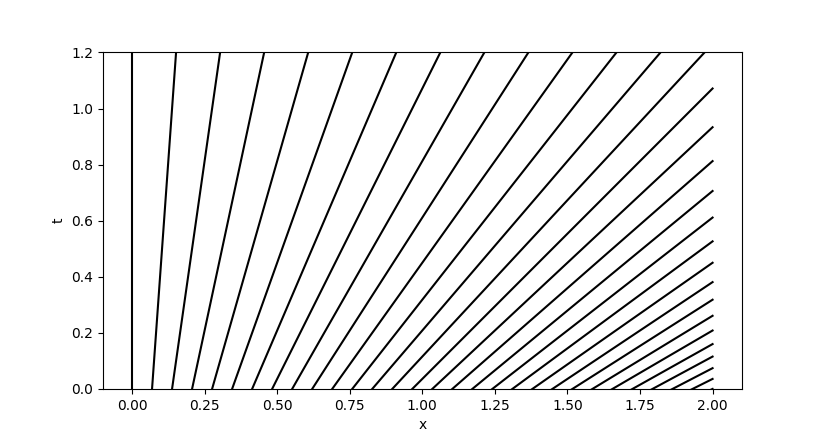
\includegraphics[scale=0.5]{figures/sheet_3_burger.png} 
   \end{figure}
\end{solution}
\begin{question}
 Derive the solution to the IVP 
\end{question}
\begin{solution}
  To recap what we know : 
  \begin{align*}
		x(s) & = x_{0}*s+x_{0} \\
		t(s) & = s     \\ 
    z(s) &= u(x_{0}*s+x_{0},s) = g(x_{0})
  .\end{align*}
No for arbitrary $(x,t) \in \mathbb{R}\times \mathbb{R}$ determine the characteristic :
\begin{align*}
  x &= x_{0}+t +x_{0} \\
.\end{align*}
this implies 
\begin{align*}
 x = x_{0}*(1+t) \implies x_{0} = \frac{x}{1+t}
.\end{align*}
Which means  
\begin{align*}
  u(x,t) = g(\frac{x}{1+t} = \frac{x}{1+t}
.\end{align*}
\end{solution}
\begin{question}
 Verify this is indeed a solution  
\end{question}
\begin{solution}
 We check $u(x,0) = \frac{x}{1+0} = x = g(x)$  and : 
 \begin{align*}
   \dot{u} + u \partial_x u =  - \frac{x}{(1+t)^2}  + \frac{x}{1+t}*\frac{1}{1+t}  = 0
 .\end{align*}
\end{solution}
\begin{question}
 Explain why the method of characteristics is well-suited to solving first order PDEs that are linear in the derivatives 
\end{question}
\begin{solution}
  We can use the chain rule to reduce the problem to a system of ODEs
\end{solution}
\section{Solving PDEs}




% \section{Dont cross the streams}
Consider the PDE $\partial_x u + 2x\partial_y u  = 0$ on the domain $y>0$ with the boundary condition $u(x,0) = g(x)$
\begin{question}
  \textbf{(a)} Show that the boundary hyperplane $\{y=0\}  $ is non-characteristic at $(x,0)$, except for $x=0$.
\end{question}
\begin{solution}
Consider the PDE as a function $F(\frac{\partial u}{\partial x},\frac{\partial u}{\partial y},u(x,y),x,y)=0$   then we need to show that : 
\begin{align*}
  \partial_{p_{1}} F(p_{0},p_{1},z,x,y) \neq 0
.\end{align*}
In our case : 
\begin{align*} 
  \partial_{p_{1}} F(p_{0},p_{1},z,x,y)  = \partial_{p_{1}} \left( p_{0} + 2x p_{1} \right)   = 2x
.\end{align*}
Which as required is non zero on $(x,0)$ except for $x=0$
\end{solution}
\begin{question}
  \textbf{(b)}  What condition does the PDE impose on the boundary data g at the point $(0,0)$
\end{question}
\begin{solution}
 At the point $(0,0)$ we know $F(d \frac{g(0)}{dx},p_{1},g(0),0,0) = 0$ but 
 \begin{align*}
  F(d \frac{dg(0)}{dx},p_{1},g(0),0,0) = \frac{dg}{dx}(0) + 2*0*p_{1} =  \frac{dg}{dx}(0) = 0
 .\end{align*}
 The PDE requires g to be constant at $(0,0)$
\end{solution}
\begin{question}
  \textbf{(c)} Determine the characteristic curves of this PDE.
\end{question}
\begin{solution}
 Consider $z(s) = u(x(s),y(s))$  then : 
 \begin{align*}
   z'  = \partial_x u x' + \partial_y y' 
 .\end{align*}
 Choosing $x' = 1 $ and $y' =  2x$ aligns with the PDE such that  
 \begin{align*}
   x(s) &= s +x_{0} \\
   y(s) &= 2xs + y_{0}
 .\end{align*}
 Considering the initial condition 
 \begin{align*}
  z(0) = u(x(0),y(0)) =  u(x_{0},0)
 .\end{align*}
 Meaning $y(s) = 2xs$ this leads to : 
 \begin{align*}
   z(s) = u(x_{0}+s,2xs) = g(x_{0})
 .\end{align*}
 For $(x,y)$ we get : 
 \begin{align*}
   x_{0} &= x-s  \\
   s     &= \frac{y}{2x}
 .\end{align*}
 Such that : 
 \begin{align*}
  u(x,y)  = g(x-\frac{y}{2x})
 .\end{align*}
\end{solution}
\begin{question}
 By considering the $y$-derivative of u on the boundary hyperplane, show that there is no $\mathcal{C}^{1} $ solution with the initial data $g(x) = x$
\end{question}
\begin{solution}
% On the boundary hyperplane $H = \{y=0\}  $ we have by (a) that it is non characteristic at $(x,0)$ except for $x=0$ 
% This means that : 
% \begin{align*}
%   \frac{\partial F}{\partial p_{1}}(\frac{dg(0)}{dx},p_{1},z,0,0) = 0 
% .\end{align*}
% Which requires $\frac{dg}{dx}$ to be constant ? idk dude, i think the issue is that g needs to be constant but it isnt
By (b) we know that the PDE requires $g'= 0$ at $(0,0)$ but for initial data $g(x) = x $ we get $\frac{dg}{dx}(0) = 1 \neq 0$, such that no $\mathcal{C}^{1} $ solution may exist,
other way is using that $H = \{y=0\}  $ is non-characteristic at $(0,0)$
\end{solution}

% \section{Bonus}
\begin{question}
  Calculate $(I | \triangledown \lambda ) * \begin{pmatrix} I \\ \triangledown \lambda  \end{pmatrix} $ and show that the determinant of it is equal to $\sqrt{1+\abs{\triangledown \lambda }^2} $
\end{question}
\begin{solution}
\end{solution}

% \begin{align*}
  &\text{Leon Fiethen 1728330}\\
 &\text{Janik Sperling 1728567}
.\end{align*}
\section*{Sheet 7}
Unclear if $u \in  \mathcal{C}(\mathbb{R}^{n} ) $ is $u : \mathbb{R}^{n} \to  \mathbb{R}$ or $u : \mathbb{R}^{n} \to \mathbb{R}^{n}  $, we consider the first case here
but it doesn't change any of the following proofs 
\subsection*{19. Twirling towards freedom}
Let $u \in  \mathcal{C}^{2}(\mathbb{R}^{n} ) $ be a harmonic function. Show that the following functions are also harmonic.\\[1ex]
\textbf{Note } Whenever we write $\frac{\partial v}{\partial x_i}$ we are really referring to $\tilde{x}(x)_i$  
\begin{exercise}[a]
  $v(x) = u(x+b) $ for $b \in  \mathbb{R}^{n} $ 
\end{exercise}
\begin{solution}
 Using chain rule gives 
 \begin{align*}
  \frac{\partial v}{\partial x_i}  = \frac{\partial u}{\partial x_i} *\frac{\partial (x+b)}{\partial x_i}  = \frac{\partial u}{\partial x_i }*1 
 .\end{align*}
 Second derivative gets another $* \ 1$. \\[1ex]
 Such that summing gives 
 \begin{align*}
  \triangle v =  1* \triangle u = 0
 .\end{align*}
\end{solution}
\begin{exercise}[b]
 $v(x) = u(ax)$  for $a \in  \mathbb{R}^{n} $
\end{exercise}
\begin{solution}
 Again using chain rule 
 \begin{align*}
  \frac{\partial v}{\partial x_i}  = \frac{\partial v}{\partial x_i} *\frac{\partial (ax)}{\partial x_i}  = \frac{\partial v}{\partial x_i }*a 
 .\end{align*}
 For the second derivative : 
 \begin{align*}
   \frac{\partial v}{\partial x_i}  = \frac{\partial^2 u}{\partial x_i^2} *\frac{\partial (ax)}{\partial x_i}*a  = \frac{\partial^2 u }{\partial x_i }*a^2
 .\end{align*}
 \begin{align*}
  \triangle v = a^2 \triangle u = a^2 * 0 = 0
 .\end{align*}
\end{solution}
\begin{exercise}[c]
 $v(x) = u(Rx)$ for $R(x_{1},\ldots,x_n) = (-x_{1},\ldots ,x_n)$ 
\end{exercise}
\begin{solution}
 Using chain rule
 \begin{align*}
   \frac{\partial v}{\partial x_i}  = \frac{\partial v}{\partial x_i} *\frac{\partial (Rx)}{\partial x_i}  = \begin{cases}
     -1 &\frac{\partial v}{\partial x_1} \text{ if } i=1\\
    &\frac{\partial v}{\partial x_i} 
   \end{cases}
 .\end{align*}
 Second derivative if $i=1$ we get another $-1$ and they cancel out s.t.
 \begin{align*}
   \frac{\partial ^2 v}{\partial x_i^2}  = \frac{\partial ^2 u}{\partial x_i^2} 
 .\end{align*}
 Summing gives 
 \begin{align*}
  \triangle v = \triangle u = 0
 .\end{align*}
\end{solution}
\begin{exercise}[d]
 $v(x) = u(Ax) $ for any orthogonal matrix $A \in  O(\mathbb{R}^{n} )$ 
\end{exercise}
\begin{solution}
  Note $(Ax)_i = \sum_{j=1}^{n} A_{ji}x_j $ such that using the chain rule 
\begin{align*} 
  \frac{\partial v}{\partial x_i}  = \frac{\partial u(Ax)}{\partial (Ax)_i}\frac{\partial Ax}{\partial x_i}  = \triangledown u *\underbrace{A_i}_{i\text{-th col}}
.\end{align*}
We get the gradient of $u$ since we take the derivative of $u$ with respect to $(Ax)_i$\\[1ex]
Second derivative 
\begin{align*}
  \frac{\partial}{\partial x_i} \frac{\partial v}{\partial x_i} =  \frac{\partial}{\partial (Ax)_i} \triangledown u(Ax) * A_i * \frac{\partial Ax}{\partial x_i}   = \triangledown * (\triangledown u*A_i)A_i 
.\end{align*}
Note since $A$ is orthogonal we get $A A^{T} = \cha $, writing out the terms as sum for clarity 
\begin{align*}
  \sum_{j,k = 1}^{n} \frac{\partial ^2 u}{\partial x_j \partial x_k} A_{ji}A_{ki}  = \sum_{i=1}^{n} \frac{\partial ^2 u }{\partial x_i^2}  = 0
.\end{align*}
\end{solution}
\newpage
\subsection*{20. Harmonic Polynomials in Two Variables}
\begin{exercise}[a]
 Let $u \in  \mathcal{C}^{\infty}(\mathbb{R}^{n} ) $ be a smooth harmonic function. Prove that any derivative of u is also harmonic
\end{exercise}
\begin{solution}
First note that $u^{(k)}(x_{0})  \in  \mathcal{C}^{\infty}(\mathbb{R}^{n} ) $ for any $k \in  \mathbb{N}$ \\ 
and $x_{0} \in  \mathbb{R}^{n} $ \\
\textbf{IA:} $k=1$
\begin{align*}
  \triangle (u^{(1)} ) = \begin{pmatrix} \frac{\partial ^2}{\partial x_i^2} , \ldots  , \frac{\partial ^2}{\partial x_i^2} \end{pmatrix}  \begin{pmatrix} \frac{\partial u(x_{0})}{\partial x_1} \\ \vdots \\ \frac{\partial u(x_{0})}{\partial x_n}\end{pmatrix}  = \sum_{i=1}^{n}  \frac{\partial ^2}{\partial x_i^2}* \frac{\partial u}{\partial x_i}  
.\end{align*}
The order of differentiation does not matter such that we get 
\begin{align*}
  \triangle (u^{(1)} ) = \frac{d}{dx} (\triangle u^{1} ) = 0
.\end{align*}
\textbf{IV:} Suppose the statement holds for $k \in  \mathbb{N}$ \\
\textbf{IS:} $k \to k+1$ \\
We know that $u^{(k)} \in \mathcal{C}^{\infty}(\mathbb{R}^{n} )  $ is harmonic by IV. such that by relabeling 
$u^{(k)}  \coloneqq  v \in \mathcal{C}^{\infty}(\mathbb{R}^{n} ) $ we can again apply the argument from the IA. which concludes the proof
\end{solution}
\begin{exercise}[b]
 Choose any positive degree n. Consider the complex valued function $f_n : \mathbb{R}^{2} \to  \mathbb{C}$ given by
$f_n(x, y) = (x+iy)^{n}$  and let $u_n(x, y)$ and $v_n(x, y)$ be its real and imaginary parts respectively.
Show that $u_n$ and $v_n$ are harmonic. 
\end{exercise}
\begin{solution}
  Treating the Laplacian in $\mathbb{C}$ as we do in $\mathbb{R}$ 
  \begin{align*}
    \partial_x f_n  &= n(x+iy)^{n-1} \\
    \partial_y f_n  &= n*i(x+iy)^{n-1} 
  .\end{align*}
  Then 
  \begin{align*}
    \triangle f_n &= n(n-1)(x+iy)^{n-2}  +(i^2n(n-1)(x+iy)) \\
    &= n(n-1)*\left( (x+iy)^{n-2} - (x+iy)^{n-2}   \right)  \\
    &= 0
  .\end{align*}
  Since $u_n,v_n$ are real and imaginary part , their Laplacian must be 0 as well.
  % We identify $\mathbb{C}$ with $\mathbb{R}^{2} $ by $ \phi  :\ \mathbb{R}^{2} \to  \mathbb{C} \ : \ (x,y) \mapsto x +iy$\\[1ex]
  % Then we consider $f_n = \phi \circ \tilde{f}_n$ where
  % \begin{align*}
  %   \tilde{f}_n \ : \ \mathbb{R}^{2}   \to  \mathbb{R}^{2}  \ (x,y) \mapsto \begin{pmatrix} u_n(x,y) \\ v_n(x,y) \end{pmatrix} 
  % .\end{align*}
  % Applying the Laplacian operator to   $\tilde{f}_n$ 
  % \begin{align*}
  %   \triangledown * (\triangledown \tilde{f}_n) =  \begin{pmatrix} \frac{\partial ^2 u}{\partial x^2}+ \frac{\partial ^2 u}{\partial y^2} , \frac{\partial ^2 v}{\partial x^2}+ \frac{\partial ^2 v}{\partial y^2}  \end{pmatrix} 
  % .\end{align*}
  % Now if we apply the chain rule to 
  % \begin{align*}
  %   \phi \circ \tilde{f}
  % .\end{align*}
  % Consider the Term 
  % \begin{align*}
  %   \frac{\partial \phi }{\partial \tilde{f}}  = (1,i)
  % .\end{align*}
  % And 
  % \begin{align*}
  %   \frac{\partial \phi }{\partial \tilde{f}}  = (1,i)
  % .\end{align*}
%   Using (a) and induction ($u_n$,$v_n$ harmonic) gives \\[1ex]
%   \textbf{IA} $n=1$ : 
%   \begin{align*}
%     f_1(x,y) = x+iy
%   .\end{align*}
%   Such that
%   \begin{align*}
%     u_1(x,y) = x \\
%     v_1(x,y) = y
%   .\end{align*}
%   Clearly $u$ and $v$ are twice differentiable (smooth even)  and 
%   \begin{align*}
%     \triangle u_1 &= 0 \\
%     \triangle v_1 &= 0
%   .\end{align*}
% \textbf{IV} suppose the statement holds for arbitrary  $n \in  \mathbb{N}$ \\
% \textbf{IS} $n\to n+1$ 
% We get 
% \begin{align*}
%   f_{n+1} = u_{n+1} + i*v_{n+1} 
% .\end{align*}
% Then consider 
% \begin{align*}
%   u_{n+1} = u_n + p(n)
% .\end{align*}
\end{solution}
\begin{exercise}[c]
 A  homogeneous polynomial of degree $n$ in two variables is a polynomial of the form 
 \begin{align*}
  p = \sum a_k x^{k}y^{n-k}  
 .\end{align*}
 Show that $\partial_x p$ and $\partial_y p$ are homogeneous of degree $n-1$
\end{exercise}
\begin{solution}
  Calculating 
  \begin{align*}
    \partial_x p = \frac{\partial}{\partial x} \sum_{k=0}^{n}  a_k x^{k} y^{n-k}   = \sum_{k=0}^{n} k*a_kx^{k-1}y^{n-k}  
  .\end{align*}
  For $k=0$ we have $ k*a_k = 0$ such that the first term vanishes
  \begin{align*}
    \sum_{k=0}^{n} k a_k x^{k-1}y^{n-k} = \sum_{k=1}^{n} k a_k x^{k-1}y^{n-k} = \sum_{i=0}^{n-1} (i+1)a_{i+1}x^{i}y^{(n-1)-i}   
  .\end{align*}
  For the case $\partial_y$ we get the term $(n-k)*a_k$ which is 0 for $k=n$  such that the last term of our sum vanishes 
  and the degree is reduced by 1 \\[1ex]
\end{solution}
\begin{exercise}[d]
 Show that such a homogeneous polynomial of degree n is harmonic if and only if it is a linear combination of $u_n$  and $v_n$
\end{exercise}
\begin{solution}
 "$\Leftarrow$":  Let $p$ be a linear combination of $u_n$ and $v_n$ then by (b) we know $u_n$ and $v_n$ are harmonic, since 
 the Laplacian is a linear operator, we conclude $p$ must also be harmonic. \\[1ex]
 Other direction is missing
\end{solution}
\subsection*{Louisville's Theorem}
Liouville’s theorem (3.9 in the script) says that if $u$ is bounded and harmonic, then $u$ is constant.
In this question we give a geometric proof in $\mathbb{R}^{2} $ using globular means defined when $B(x, r) \subset  \Omega $
through
\begin{align*}
  \mathcal{M}[v](x,r) = \frac{1}{\omega_nr^{n} } \int_{B(x,r)}v(y) dy
.\end{align*}
Recall from Theorem 3.5 that if u is harmonic then it obeys $u(x) = \mathcal{M}[u](x, r)$.
\begin{exercise}[a]
Consider two points $a,b$ in the plane which are distance $2d$ apart. Now consider two balls,
both with radius $r>d$, centered on the two points respectively. Show that the area of the intersection is 
\begin{align*}
  \text{area} B(a,r) \cap B(b,r) = 2r^2 a\cos(dr^{-1} ) - 2d\sqrt{r^2-d^2} 
.\end{align*}
\end{exercise}
\begin{solution}
  W.l.o.g we may assume $a = (0,0)$  and $b=(2d,0)$, otherwise we just shift the plane to be centered at a first and rotate (both volume preserving) \\[1ex]
  In that case we can solve for the points of intersection by 
  \begin{align*}
    x^2+y^2 = r^2 = (x-2d)^2 + y^2
  .\end{align*}
  Such that 
  \begin{align*}
    x^2 -(x-2d)^2 &= 0 \\
    x^2 -(x^2-4dx+4d^2) &= 0 \\
    4dx - 4d^2 &= 0 \\
    x = d
  .\end{align*}
  And y 
  \begin{align*}
    d^2 + y^2 = r^2 \implies y = \pm \sqrt{r^2-d^2} 
  .\end{align*}
  Now either by integrating we get 
  \begin{align*}
    x^2+y^2 = r^2 \implies x = \sqrt{r^2-y^2} 
  .\end{align*}
  \begin{align*}
    2*\left( \int_{-\sqrt{r^2-d^2} }^{\sqrt{r^2-d^2} } \sqrt{r^2-y^2}  dy - 2d*\sqrt{r^2-d^2}  \right) 
  .\end{align*}
  Or the prettier way \newpage
  \hspace{0mm}\\
  We can get the light-green area by calculating the area of the triangle and subtracting it from the area of the sector and multiplying by 4, this gives the following \\[1ex]
  Triangle area
  \begin{align*}
    \frac{1}{2} *d*\sqrt{r^2-d^2}  
  .\end{align*}
  Sector area , since $\theta = \cos^{-1}(\frac{d}{r})$ and the area of the sector is proportional to the angle where $\theta =2\pi $ 
  gives the full circle we get 
  \begin{align*}
    \frac{r^2 \theta }{2}
  .\end{align*}
  Putting it together 
  \begin{align*}
    &4*\left(\frac{r^2 \cos^{-1}(\frac{d}{r})}{2} -  \frac{d}{2}\sqrt{r^2-d^2} \right)\\
    &=2r^2\cos^{-1}(dr^{-1}) - 2d\sqrt{r^2-d^2} 
  .\end{align*}
  \begin{center}
    \begin{figure}[H] 
      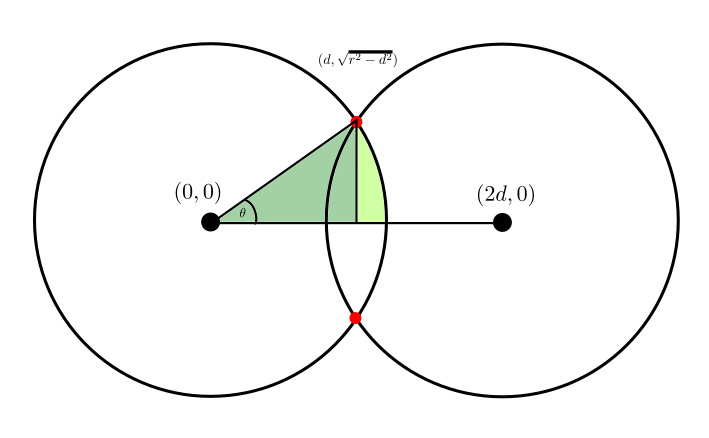
\includegraphics[scale=1]{figures/area_alternative.png}
   \end{figure} 
  \end{center}
\end{solution}
\newpage
\begin{exercise}[b]
 Suppose that $v$ is a bounded function on the plane $-C \le v(x) \le C$  for all x and some constant C. Show that 
 \begin{align*}
   \abs{\mathcal{M}[v](a,r) - \mathcal{M}[v](b,r)} \le \frac{2C}{\omega_2}(\pi -2a\cos(\frac{d}{r})) - \frac{2d}{r}\sqrt{1-d^2r^2} 
 .\end{align*}
\end{exercise}
\begin{solution}
  We get
  \begin{align*}
    \abs{\mathcal{M}[v](a,r) - \mathcal{M}[v](b,r)} &=\frac{1}{\omega_2r^{2} }  \abs*{\left(  \int_{B(a,r)} v(y) dy -  \int_{B(b,r)} v(y) dy \right)} \\
  .\end{align*}
  leaving the constant 
\begin{align*} 
  &=\abs*{\left(  \int_{B(a,r) \setminus B(b,r)} v(y) dy -  \int_{B(b,r) \setminus B(a,r)} v(y) dy \right)} \\
  &\le   \int_{B(a,r) \setminus B(b,r)} \abs*{v(y)} dy +  \int_{B(b,r) \setminus B(a,r)} \abs{v(y)} dy \\
  &\myS{def.}{\le } \int_{B(a,r) \setminus B(b,r)} C dy -  \int_{B(b,r) \setminus B(a,r)} C dy \\
.\end{align*}
Then by drawing a picture and looking at it we know 
\begin{align*}
  \text{area}(B(a,r) \setminus B(b,r)) + \text{area}(B(a,r) \setminus B(b,r)) =  2\pi r^2 - 2*\text{area}(B(a,r) \cap B(b,r))
.\end{align*}
Using (a)
\begin{align*}
  \abs{\mathcal{M}[v](a,r) - \mathcal{M}[v](b,r)} \le \frac{2C}{\omega_2}*\left(\pi - 2\cos^{-1}(\frac{d}{r})+\frac{2d}{r^2}\sqrt{r^2-d^2}  \right) 
.\end{align*}
\end{solution}
\begin{exercise}[c]
 Let $u \in  \mathcal{C}^{2}(\mathbb{R}^{2} ) $ be a bounded harmonic function. Complete the proof that u is constant 
\end{exercise}
\begin{solution}
 By Theorem 3.5 we know that
 \begin{align*}
   u(x) = \mathcal{M}[u](x,r)
 .\end{align*}
Picking any points $a,b \in  \mathbb{R}^{2} $ we check the distance
\begin{align*}
  \abs{u(a)-u(b)} = \abs{\mathcal{M}[u](a,r) - \mathcal{M}[u](b,r)} \le C(r,d)
.\end{align*}
Where $r >d \coloneqq  \|a-b\|$ , i.e 
\begin{align*}
  \lim_{h \to 0} \frac{\abs{u(a+h) - u(a)}}{h} &= \lim_{h \to 0} \frac{\abs{\mathcal{M}[u](a+h,r(h)) - \mathcal{M}[u](a,r(h))}}{h}\\
                                               &\le \lim_{h\to 0} \frac{1}{h} * C(r(h),h) \\
                                               &=0
.\end{align*}
Where $C(r(h),h) \to  0$ as $h\to 0$  , thus $u$ must be constant if it is bounded and harmonic
\end{solution}
\subsection*{Weak Tea}
In this question we try to generalise the idea of spherical means to distribution in the way 
suggested in the lectures. Let $\lambda_{\epsilon } : \mathbb{R} \to  \mathbb{R}$ be the standard mollifier and define a sphere mollifier 
\begin{align*}
  \Lambda_{x,r,\epsilon}(y) = \frac{\lambda_{\epsilon }(\abs{y-x}-r)}{n \omega_{n}\abs{y-x}^{n-1} }
.\end{align*}
\begin{exercise}[a]
  Describe the support of $\Lambda_{x,r,\epsilon }$ 
\end{exercise}
\begin{solution}
  By definition it is all $y$ such that $\Lambda_{x,r,\epsilon }(y) \neq 0$ i.e all y such that $\abs{y-x} - r \in \supp \lambda_{\epsilon} \coloneqq \overline{B(0,\epsilon)} $,
  Which gives
  \begin{align*}
    \abs{y-x} -r \le  \epsilon  \implies \abs{y-x} \le \epsilon + r
  .\end{align*}
  \begin{align*}
    y \in B(x,\epsilon +r)
  .\end{align*}
\end{solution}
\begin{exercise}[b]
  We may try to define the spherical mean of a distribution $F$ as $\lim_{\epsilon  \to  0} F(\Lambda_{x,r,\epsilon })$. However
this does not always exist. Let $G$ be the distribution in Exercise 17(d), submanifold inte-
gration on the unit circle. Show that $G(\Lambda_{0,1,\epsilon }) = \lambda_{\epsilon }(1)$ and therefore the limit does not
exist.
\end{exercise}
\begin{solution}
  First we can check that indeed  $\Lambda \in  \mathcal{C}^{\infty}_0 $ such that $G(\Lambda_{0,1,\epsilon })$ is valid 
 \begin{align*}
   \Lambda_{0,1,\epsilon } = \frac{\lambda_{\epsilon}(\abs{y}-1)}{2 \omega_2 \abs{y}}
 .\end{align*}
 We have $C \coloneqq  \{x^2+y^2 = 1\}  $ i.e $C \coloneqq  \partial B(0,1)$ then 
 \begin{align*}
   G(\Lambda_{0,1,\epsilon }) &= \int_{\{x^2+y^2=1\}  } \frac{\lambda_{\epsilon}(\abs{y}-1)}{2 \omega_2 \abs{y}} d\sigma\\
                              &= \int_{\partial B(0,1)}\frac{\lambda_{\epsilon}(0)}{2\omega_2} d\sigma  = \lambda_{\epsilon }(0)
 .\end{align*}
 If we didn't  shift by $r=1$ it would be 1. For $\epsilon  \to 0$ we have $\lambda_{\epsilon }(0) \to \infty$
\end{solution}
\begin{exercise}[c]
  Show that the limit $\lim_{\epsilon \to 0} F(\Lambda_{x,r,\epsilon })$ 
\end{exercise}
\begin{solution}
 Let $F$ be a harmonic distribution i.e $\triangle F = 0$ then  F has the weak mean value property by Theorem 3.6
 and we know that $F$ vanishes on any test function with $\int \psi d\mu = 0$ where $\psi \in  \mathcal{C}^{\infty}_0((0,r)) $\\
 We know that necessarily  we have 
\begin{align*}
 \int_\Omega  \Lambda_{x,r,\epsilon }  d\mu = 1 
.\end{align*} 
Choose any test function $\phi $ such that its integral is 1  then $\tilde{\phi } = \phi - \Lambda_{x,r,\epsilon}$  
\begin{align*}
  \int_\Omega  \tilde{\phi } = 0
.\end{align*}
Since distribution are linear operators 
\begin{align*}
  0 = F(\tilde{\phi }) = F(\phi) - F(\Lambda_{x,r,\epsilon })
.\end{align*}
Thus the limit exists.
\end{solution}
\section{Tutorial}
\subsection*{19.}
WE can generalise the argument for all linear transformations
\begin{align*}
  y = Ax +b   \implies y_j = \sum_{k}A_{jk}x_k + b_j
.\end{align*}
Then define 
\begin{align*}
  v(x) = u(Ax +b)
.\end{align*}
then by chain rule 
\begin{align*}
  \frac{\partial v}{\partial x_i}  &= \sum \frac{\partial u}{\partial y_{i}} \frac{\partial y}{\partial x_i}  \\
                                   &= \sum_{l} \frac{\partial u}{\partial y_l}  A_{li}
.\end{align*}
And 
\begin{align*}
  \frac{\partial ^2 v}{\partial x_j \partial x_i}  &= \sum \frac{\partial }{\partial x_j}  \frac{\partial u}{\partial y_{i}} A_{li} \\   
                                                   &= \sum_{l,m} \frac{\partial u}{\partial y_m \partial y_l}  A_{mj}A_{li}
.\end{align*}
Then we get for the laplacian
\begin{align*}
  \triangle v &= \sum_{i} \frac{\partial ^2 v}{\partial x_i^2}  \\
              &= \sum_{l,m} \frac{\partial u}{\partial y_m \partial y_l } (\sum A_{mi} A_{li})
              &= \triangle u 
.\end{align*}
Last equality for $A \in  O(M)$, writing it out as a matrix 
\begin{align*}
  H(v)_{ij} = \sum_{l,m} H(u)_{m,l}A_{mj}A_{li}
.\end{align*}
This is the same  as 
\begin{align*}
  \sum_{m,l} A_{jm}^{T} H(u)_{ml} A_{li}
.\end{align*}
Then 
\begin{align*}
  \triangle v &= \text{trace}(H(v)) \\
              &= \text{trace}(A^{T}H(u)A ) \\
              &= \text{trace}(A A^{T}H(u) )
.\end{align*}
\subsection*{20}
All Harmonic polynomials have a saddle point at $(0,0)$ \\[1ex]
$P^{d} $  homoegnous degree d 
\begin{align*}
  P^{D} = \begin{pmatrix} n+d-1 \\ n-1 \end{pmatrix}  
.\end{align*}
Then 
\begin{align*}
  \triangle : P^{d} \to P^{d-2}  
.\end{align*}
For $p = x_{1}^2x_{2}x_{3}^2$ we get
\begin{align*}
  \triangle p =  2x_{2}x_{3}^2  + 0 + 2x_{1}^2x_{2} 
.\end{align*}
$\triangle$ is surjective since 
\begin{align*}
 \dim \ker \triangle = \begin{pmatrix} n+d-1 \\ n-1 \end{pmatrix}   - \begin{pmatrix} n+d-3 \\ n-1 \end{pmatrix} 
.\end{align*}
n choose k for the amount of harmonic polynomials, harmonic functions are smooth and indeed also harmonic i.e 
they are equal to their taylor series i.e theyre polynomials\\
If $u$ has the MVP for spheres S it also has it for the globular mean 
\begin{align*}
  M[u](x,r)  &= \frac{n}{r^{n} } \int_0^{r} u(x)s^{n-1}   ds \\
             &= \frac{n}{r^{n} } u(x) \frac{1}{n} [s_n]_{0}^{r}  \\
             &= u(x)
.\end{align*}
Other direction if $u$ has MVP for M  then 
\begin{align*}
  u(x) = M[u](x,r)
.\end{align*}
And 
\begin{align*}
  \frac{1}{n}r^{n} u(x) &= \int_0^{r} s^{n-1}S[u](x,s)    ds \\
  \frac{1}{n}n r^{n-1}u(x)&= r^{n-1}S[u](x,r)  
.\end{align*}
Proof of 21, is to lower bound the are of the Lens created by the intersection of two circles by 
using the circle that fits inside it, when $r \to \infty$ the shared values of both circles become
very similar and thus their difference should tend to 0\\[1ex]
Small note in 
\begin{align*}
  \Lambda = \frac{\lambda_{\epsilon }(\abs{y-x})}{n\ldots }
.\end{align*}
The $\abs{*}$ refers to the norm in the relevant dimension, i.e $y \in  \mathbb{R}^{n} $ and $x \in  \mathbb{R}^{n} $


% 
\begin{align*}
  &\text{Leon Fiethen 1728330}\\
 &\text{Janik Sperling 1728567}
.\end{align*}
\section*{Sheet 7}
\subsection*{23}
\begin{question}
Suppose that $u \in  \mathcal{C}^2(\mathbb{R}^{2} )$ is harmonic with 
critical point at $x_{0}$. Assume the Hessian of $u$ has non-zero determinant. Show 
that $x_{0}$ is a saddle point. Explain the connection
to the maximum principle  
\end{question}
\begin{solution}
  Since $u \in  \mathcal{C}^2(\mathbb{R}^{2} )$  is harmonic and assume 
  assume $x_{0}$ is a maximum, then by the maximum principle $u$ must be constant and $u' = 0$, 
  therefore $H(u)$ must have 0 determinant too, for minima we argue that $x_{0}$ minima of $u$ implies
  a maxima of $-u$ and the same argument applies. \\[1ex]
  It follows if $u$ has a Hessian with non zero determinant it must have a saddle point at $x_{0}$
\end{solution}
\subsection*{24}
Let $\Omega \subset  \mathbb{R}^{n} $ be an open and connected region. A continuous function $v : \overline{\Omega } \to \mathbb{R} $
is called subharmonic if for all $x \in  \Omega $ and $r>0$ with $B(x,r) \subset  \Omega $ it lies below its spherical mean 
\begin{align*}
  v(x) \le  \mathcal{S}[v](x,r)
.\end{align*}
\begin{question}[a]
 Prove that every subharmonic function obeys the maximum-principle i.e. 
 if the maximum of $v$ can be found inside $\Omega $ then $v$ is constant
\end{question}
\begin{solution}
 Suppose $x_{0} \in  \Omega $ is the maximum of $v$ then on a ball of radius $r>0$ around $x_{0}$ we have
 \begin{align*}
   0 \ge  v(x_{0}) - S[v](x_{0},r) = \frac{1}{C} \int_{\partial B(x_{0},r)} v(x_{0}) - v(y) d\sigma(y) \ge  0
 .\end{align*}
 As from $x_{0}$ maxima it follows that  for $\forall  y \in  B(x_{0},r)$ 
 \begin{align*}
  v(x_{0}) - v(y) \ge 0
 .\end{align*}
 We conclude that for all $y \in  \partial B(x_{0},r)$ 
 \begin{align*}
  v(x_{0}) = v(y)
 .\end{align*}
 Now suppose there exists $y_{1} \in B(x_{0},r)  $ such that $\abs{v(y_{1})-v(x_{0})} > 0$ then by continuity we have 
 $\forall  x \in  B(y_{1},r)$ also (where $r>0$ is sufficiently small )$\abs{v(x)-v(x_{0})} > 0$ such that 
 \begin{align*}
   0 &< \frac{1}{C} \int_{B(y_{1},r)} v(x_{0}) - v(y) \\
     &\le \frac{1}{C} \int_{B(y_{1},r)} S[v](x_{0},r) - v(y) d\mu(y)\\ &
     = S[v](x_{0},r) - \frac{1}{C} \int_{B(y_{1},r)} v(y) d\mu(y)  
 .\end{align*}
 for $r \to 0$ we must have 
 \begin{align*}
   0 < S[v](x_{0},r) - \frac{1}{C} \int_{B(y_{1},r)} v(y) d\mu(y) \le x_{0}-y_{1} \ge  0
 .\end{align*}
 a contradiction.  (idk about this fully tbh). \\[1ex]
 Now we know that if $v$ attains a maxima $x_{0}$ it must be constant on a small ball centered at $x_{0}$ with $r>0$. 
 By compactness we can cover $\overline{\Omega }$  by finite many balls of radius $\frac{r}{2}>0$ 
 \begin{align*}
  B(\gamma_{1},\frac{r}{2}),\ldots ,B(\gamma_n,\frac{r}{2})
 .\end{align*}
 Pick $\gamma_{1} = x_{0}$ then v is constant on the first ball and the next center $\gamma_{2}$ must necessarily be contained in the ball 
 $B(x_{0},r)$ such that $v$ is also constant on this ball, by repeating this argument we get that $v$ must be constant on all balls.
\end{solution}
\begin{question}[b]
 Suppose that $v$ is twice continuous differentiable. Show that $v$ is subharmonic if and only 
 if $- \Delta v \le 0$ in $\Omega$
\end{question}
\begin{solution}
 Assume first that $-\Delta v \le 0$ in $\Omega$ and define 
 \begin{align*}
   \tilde{v}(r) = S[v(x)-v](x,r) 
 .\end{align*}
 for $x \in  \mathbb{R}$ then by the divergence theorem we get that 
 \begin{align*}
   \frac{d}{dr}\tilde{v}(r)  =  -\frac{1}{C} \int_{B(x,r)} \Delta v d\mu
 .\end{align*}
 By assumption 
 \begin{align*}
   \frac{d}{dr} \tilde{v}(r)  \le  0
 .\end{align*}
 Such that we must have for all $\tilde{r} \le r $
 \begin{align*}
   \tilde{v}(r) - \tilde{v}(\tilde{r}) \ge 0
 .\end{align*}
 But 
 \begin{align*}
   \tilde{v}(r) - \tilde{v}(\tilde{r})  &= v(x) - S[v](x,r) - (v(x) - S[v](x,\tilde{r})) \\
                                          &= S[v](x,\tilde{r}) - S[v](x,r) 
                                          &\le 0
 .\end{align*}
 i.e. 
 \begin{align*}
   S[v](x,\tilde{r}) \le S[v](x,r)
 .\end{align*}
 but by continuity of $v$ for $\tilde{r}\to 0$  we have
 \begin{align*}
   v(x) \le S[v](x,r)
 .\end{align*}
 We may extend this argument for $\forall  x \in  \Omega $ and $\tilde{r}>0$ such that $B(x,\tilde{r}) \subset  \Omega $ since we can cover
 $\Omega $ by finite many $r$ Balls.\\[1ex]
 Now assume $v$ is sub harmonic then we have for $x \in  \Omega $ and $\forall r>0$ such that
 the ball $B(x,r) \subset  \Omega $ that
 \begin{align*}
   \tilde{v} \le  0 
 .\end{align*}
 and we get again by divergence theorem that 
 \begin{align*}
   \frac{d}{dr} \tilde{v} = \frac{1}{C} \int_{B(x,r)} - \Delta v(y) d\mu(y)
 .\end{align*}
 If $ - \Delta v > 0 $ on $B(x,r)$  then $\frac{d}{dr} \tilde{v}  > 0  $ and 
 \begin{align*}
   S[v](x,r) \le  S[v](x,\tilde{r} )
 .\end{align*}
 which is a contradiction if we take $\tilde{r} \to 0 $ idk cuh.
\end{solution}
\begin{question}[c]
 Let $u : \overline{\Omega } \to  \mathbb{R} $  be a harmonic function. Show that $\|\nabla u\|^2$ is subharmonic
\end{question}
\begin{solution}
 To show that 
 \begin{align*}
  v \coloneqq  \|\nabla u \|^2 \ : \ \overline{\Omega } \to  \mathbb{R} \ x \mapsto \|\nabla u(x)\|^2 
 .\end{align*}
 is subharmonic we show by (b)  $-\Delta v \le 0$ 
 \begin{align*}
   \Delta v =  \Delta \|\nabla v\|^2 &= \nabla * \nabla \|\nabla v\|^2 \\
                                     &=  \sum_{j=1}^{n} \frac{\partial}{\partial x_j} * \sum_{i=1}^{n} \frac{\partial ^2 u}{\partial x_j \partial x_i}  \\
 .\end{align*}
 First recognize that 
\end{solution}



% \begin{align*}
  &\text{Leon Fiethen 1728330}\\
 &\text{Janik Sperling 1728567}
.\end{align*}
\section*{Sheet 9}
\subsection*{27. It's not easy being green}
\begin{exercise}
Suppose that $\Omega $ is a bounded domain. Prove that there is at most one Green's function on $\Omega $  
\end{exercise}
\begin{proof}
  Since $\Omega $ is bounded by using the  weak maximums principle and  using property (i) of Greens function.\\[1ex]
Assume two Green's functions for $\Omega $ $G,\tilde{G} $ exist then 
\begin{align*}
  u(y) &= G(x,y) - \tilde{G}(x,y) = G(x,y)-\tilde{G}(x,y) + (\underbrace{\Phi(x-y) - \Phi(x-y)}_{=0}) \\
       &= G(x,y)-\Phi(x-y)  - (\tilde{G}(x,y) - \Phi(x-y) )
.\end{align*}
Then $u(y)$ is harmonic by 3.18 (i) and by the weak maximum principle we must have $u(y)=  0$ 
\end{proof}
\begin{exercise}
  On the other hand, suppose that $\Omega $  has Green's function $G_{\Omega }$ and that there exists a non-trivial solution to the Dirichlet problem
  \begin{align*}
    \Delta u  = 0 \quad u \rvert_{\partial \Omega } = 0
  .\end{align*}

\end{exercise}
  \begin{proof} 
  We search for a function that satisfies properties (i) and (ii) from 3.18, since $u$ is non-trivial 
  \begin{align*}
    \tilde{G}(x,y) = G(x,y) + u(y)  \neq G(x,y)
  .\end{align*}
  and we check (i) 
  \begin{align*}
    y \mapsto \tilde{G}(x,y)  - \Phi(x-y) =  (G(x,y)-\Phi(x-y)) + u(y)
  .\end{align*}
  Both parts extend to a harmonic function  for $x \in  \Omega $ , first half  by virtue of being a Green's function , second part is harmonic by properties of being a result to the Dirichlet Problem.\\[1ex]
  For (ii) we check for $y \in  \partial \Omega $
  \begin{align*}
    y \mapsto \tilde{G}(x,y)  - \Phi(x-y) =  G(x,y) + u(y)
  .\end{align*}
  is $0$ since $G$ is a  Greens function and we have $u \rvert_{\partial \Omega } = 0$. 
  It follows that $\tilde{G} $ is a second Greens Function.
  \end{proof}
\subsection*{28. Do nothing by halves}
Let $H^{+}_1  = \{x = (x_{1},\ldots ,x_n)\in  \mathbb{R}^{n} | x_{1} >0 \}   $ be the upper half space and\\
$H^{0}_1  = \{x = (x_{1},\ldots ,x_n)\in  \mathbb{R}^{n} | x_{1} =0 \}   $
be the dividing hyperplane. We call $R_1(x)  = (-x_{1},x_2,\ldots ,x_n)$ reflection in the plane $H^{0} $
\begin{exercise}[a]
  Let $u \in  \mathcal{C}^{2}(\overline{H_1^{+} } ) $ be a harmonic function that vanishes on $H_1^{0} $. Show that the function 
  \begin{align*}
    v : \mathbb{R}^{n} \to  \mathbb{R} \ x \mapsto \begin{cases}
      u(x) &\text{ for } x_{1}\ge 0\\
      -u(R_1(x)) &\text{ for } x_{1}<0\\
    \end{cases} 
  .\end{align*}
  is harmonic
\end{exercise}
\begin{proof}
 We want to check that 
 \begin{align*}
  \Delta v = 0
 .\end{align*}
 We know (by past exercise sheet) that if  $u$ is harmonic then $u(R_{1}(x))$ is harmonic also, such that
 $v \rvert_{x_{1}>0}$ and $v \rvert_{x_{1}<0}$ are both harmonic.\\[1ex]
 We check the partial derivatives, at $x_{1}>0$ we have
 \begin{align*}
   \frac{\partial v}{\partial x_i}&=  \frac{\partial u}{\partial x_i}\\
  \frac{\partial ^2 v}{\partial x_i^2}&=  \frac{\partial ^2 u}{\partial x_i^2}
 .\end{align*}
 At $x_1 <0$
 \begin{align*}
   \frac{\partial v}{\partial x_i}&=  - \frac{\partial u(R_{1}(x))}{\partial x_i}  \\
   \frac{\partial v}{\partial x_1} &= \frac{\partial u(R_{1}(x))}{\partial x_1} 
 .\end{align*}
 and 
 \begin{align*}
  \frac{\partial ^2 v}{\partial x_i^2} &= - \frac{\partial ^2 u(R_{1}(x))}{\partial x_i^2}  \\
   \frac{\partial ^2 v}{\partial x_1^2} &= - \frac{\partial ^2 u(R_{1}(x))}{\partial x_1^2}  
 .\end{align*}
 i.e for $i\neq 1$ in the first partial derivative we should get a problem 
 \begin{align*}
   \lim_{x_1 \to 0^{+}  }\frac{\partial v}{\partial x_i}  \neq  \lim_{x_1 \to 0^{-}  }\frac{\partial v}{\partial x_i} \Leftrightarrow \lim_{x_1 \to 0^{+}  }\frac{\partial u}{\partial x_i}  &\neq  \lim_{x_1 \to 0^{-}  } -\frac{\partial u}{\partial x_i}
 .\end{align*}
 But since $u$ is continuous and vanishes on $H_1^{0} $ we have that both sides of the limit are zero for $i\neq 1$, i.e we get 
 \begin{align*}
   \lim_{x_1 \to 0^{+}  }\frac{\partial v}{\partial x_i}  =  \lim_{x_1 \to 0^{-}  }\frac{\partial v}{\partial x_i} 
 .\end{align*} 
 We get that the partial derivatives of $v$ extend continuous to $x_{1}=0$ and that $v$ is harmonic.
\end{proof}
\begin{exercise}[b]
 Show that Green's function for $H_1^{+} $  is 
 \begin{align*}
  G(x,y) = \Phi(x-y) - \Phi(R_1(x)-y)
 .\end{align*}
\end{exercise}
\begin{proof}
 We check (i)  and (ii), For (i) we first note
 \begin{align*}
 G(x,y) - \Phi(x-y) =  -\Phi(R_1(x)-y)
 .\end{align*}
 we check for singularity at $R_1(x) = y$, since $x \in  H_1^{+} $ then 
 \[R_1(x) \in  \{x=(x_{1},\ldots ,x_n) \in  \mathbb{R}^{n} \ : \ x_{1}<0 \}  \]
 but since $y \in  H^{+}_1 $, then $R_1(x) = y$ is impossible and since $\Phi$ is harmonic we get that $G(x,y) - \Phi(x-y)$ extends to a harmonic function (since we checked for the singularity).\\
 For (ii) we check for $x \in  \Omega $ and $y \in  \partial \Omega $
 \begin{align*}
 G(x,y) = \Phi(x-y) - \Phi(R_{1}(x)-y) 
 .\end{align*}
 The fundamental solution only depends on the Length  $\|R_1(x)-y\|$ is symmetric i.e.
 \begin{align*}
  \|R_1(x) - y\| = \|x-R_1(y)\|
 .\end{align*}
 Since $y \in  \partial \Omega  \coloneqq  H_1^{0} $  we get $R_1(y) = y$ and 
  \begin{align*}
    G(x,y) &= \Phi(x-y) - \Phi(R_{1}(x)-y)  \\
           &= \Phi(x-y) - \Phi(x-R_1(y))  \\
           &= \Phi(x-y) - \Phi(x-y) \\
           &= 0
 .\end{align*}
 Thus $G$ is Green's function for $H_1^{+} $
\end{proof}
\begin{exercise}[c]
 Compute the Green's function for $B^{+} $
\end{exercise}
\begin{proof}
 By 3.20 we know that 
 \begin{align*}
   G_{B(0,1)}(x,y) = \Phi(x-y) - \Phi(\abs{x}(\tilde{x}-y ))
 .\end{align*}
 where $\tilde{x} = \frac{x}{\abs{x}^2} $\\
 We know that the greens function $B(0,1)$ must be unique,then lets say we have a greens function on $B^{+} $ call it $G^{+} $, we expect 
 \begin{align*}
   G_{B(0,1)(x,y)} \rvert_{B^{+} } \equiv G^{+} 
 .\end{align*}
We consider 
\begin{align*}
  G(x,y) = \Phi(x-y) - \Phi(\abs{x}(R_1(\tilde{x})-y))
.\end{align*}
We check (i)
\begin{align*}
  G(x,y) - \Phi(x-y) =-\Phi(\abs{x}(R_1(\tilde{x})-y))
.\end{align*}
By similar argument to (b) we know the singularity is not a problem and (i) is satisfied by properties of the fundamental solution\\
For (ii) we check $x \in  B^{+}  $ and $y \in  \partial B^{+} $ , clearly the boundary $\partial B^{+} $ consists of two parts,
\begin{align*}
  \partial B^{+}   = B^{0} \cup (\partial B \cap H^{+})     
.\end{align*}
We consider the cases separately,for $x \in  B^{+} $ and $y \in  B^{0} $ 
\begin{align*}
  G(x,y) = \Phi(x-y) - \Phi(\abs{x}(R_1(\tilde{x})-y))  &= \Phi(x-y) - \Phi(\abs{x}(\tilde{x}-R_1(y)))\\
                                                        &=  \Phi(x-y) - \Phi(\abs{x}(\tilde{x} - y ))
.\end{align*}
For $x \in  B^{+} $ and $y \notin B^{0} $ it holds 
\begin{align*}
  \Phi(R_{1}(x) - y) = \Phi(x-R_{1}(y)) \neq  \Phi(x-y)
.\end{align*}
And notice it doesn't work out lol , we choose new Green's function such that the above is 0 ,
\begin{align*}
  \tilde{G}(x,y) = \Phi(x-y) - \Phi(R_{1}(x)-y)  - (\Phi(\abs{x}(\tilde{x} - y )) - \Phi(\abs{x}(R_{1}(\tilde{x})-y)))
.\end{align*}
then for $x \in  B^{+} $ and $y \in  B^{0} $
\begin{align*}
 \tilde{G}(x,y) &=   \Phi(x-y) - \Phi(R_{1}(x)-y)  - (\Phi(\abs{x}(\tilde{x} - y )) - \Phi(\abs{x}(R_{1}(\tilde{x})-y)))\\
                &=\Phi(x-y) - \Phi(x-R_1(y))  - (\Phi(\abs{x}(\tilde{x} - y )) - \Phi(\abs{x}(\tilde{x}-R_1(y))))\\
                &=\Phi(x-y) - \Phi(x-y)  - (\Phi(\abs{x}(\tilde{x} - y )) - \Phi(\abs{x}(\tilde{x}-y)))\\
                &= 0
.\end{align*}
similar argument to (b), for $y \in \partial B \cap H^{+} \subset  \partial B(0,1)$  we have by lecture 
\begin{align*}
  \|\abs{x}(\tilde{x}-y )\| = \abs{x-y}
.\end{align*}
and 
\begin{align*}
  \|\abs{x}((R_1(\tilde{x}) -y ))\| = \abs{R_1(x)-y}
.\end{align*}
Note that swapping  what $R_{1}(*)$ acts on doesn't give us anything here since $R_1(y) \neq y$.\\[1ex]
\begin{align*} 
 \tilde{G}(x,y) &=   \Phi(x-y) - \Phi(R_{1}(x)-y)  - (\Phi(\abs{x}(\tilde{x} - y )) - \Phi(\abs{x}(R_{1}(\tilde{x})-y)))\\
                &= \Phi(x-y) -  \Phi(\abs{x}(\tilde{x} - y ) +   \Phi(\abs{x}(R_{1}(\tilde{x})-y)) -\Phi(R_{1}(x)-y)\\
                &= 0
.\end{align*}
\end{proof}
\subsection*{29. Teach a man to fish}
\begin{exercise}[a]
 Using the Green's function of $H_1^{+} $  from the previous question, derive the following formal 
 integral representation for a solution of the Dirichlet problem 
 \begin{align*}
   \Delta u  = 0 \qquad u \rvert_{H_1^{0} }   = g
 .\end{align*}
 \begin{align*}
   u(x) = \frac{2x_{1}}{n \omega_n} \int_{H_{1}^{0} } \frac{g(z)}{\abs{x-z}^{n} } d \sigma(z)
 .\end{align*}
\end{exercise}
\begin{proof}
 We assume $g$ has sufficient regularity, by Greens representation we know
 \begin{align*}
   u(x) \coloneqq  \int_{H_1^{+}} G_{H_1^{+} }(x,y) f(y) d^{n}y  - \int_{H_1^{0} } g(z) \nabla_z G_{H_1^{+} } * N d \sigma(z)
 .\end{align*}
 solves the Dirichlet problem in fact  as $f \equiv 0$
\begin{align*}
  u(x) \coloneqq  - \int_{H_1^{0} } g(z) \nabla_z G_{H_1^{+} }(x,z) * N d \sigma(z)
.\end{align*}
We calculate for $n>2$ and 
\begin{align*}
 \nabla_z  G(x,z) &= \nabla_z ( \Phi(x-z) - \Phi(R_{1}(x)-z))\\
                                         &= \frac{-1}{n \omega_n}*(\frac{x-z}{\abs{x-z}^{n} } + \frac{x-z}{\abs{R_1(x)-z}^{n} })\\
.\end{align*}
If  $z \in  H_1^{0} $ we know $\abs{R_1(x) - z} = \abs{x-z}$
\begin{align*}
    \nabla_z G(x,z) &= \frac{-1}{n \omega_n}*(\frac{x-z}{\abs{x-z}^{n} } + \frac{x-z}{\abs{R_1(x)-z}^{n} })\\
                                         &= \frac{-2}{n \omega_n}\frac{x-z}{\abs{x-z}^{n} }
.\end{align*}
\begin{align*}
  u(x) &=  \frac{-2}{n \omega_n} \int_{H_1^{0} } g(z) * \frac{x-z}{\abs{z-x}^{n} }*\underbrace{N}_{=-x_{1}*\frac{1}{\abs{x-z}}} \sigma(z) \\
       &=  \frac{2x_{1}}{n \omega_n} \int_{H_1^{0} }  \frac{g(z)}{\abs{z-x}^{n} } \sigma(z)
.\end{align*}
\end{proof}
\begin{exercise}[b]
  \textcolor{Red}{Fixed the task description}\\
 Show that if $g$ is periodic that is, there is some vector $L \in  \mathbb{R}^{n-1} $)  with 
 \begin{align*}
  g(x+L) = g(x)
 .\end{align*}
 for all $x \in  \mathbb{R}^{n-1} $, then so is the solution
\end{exercise}
\begin{proof}
 We have our solution by 
 \begin{align*}
   u(x) = \frac{2x_{1}}{n \omega_n} \int_{H_1^{0} } \frac{g(z)}{\abs{x-z}^{n} } d \sigma(z)
 .\end{align*}
 We pick $\tilde{L} \in  \mathbb{R}^{n} = (0,L) $ such that $g(x+L) = g(x)$ for all $x \in  \mathbb{R}^{n-1} $ and check 
 \begin{align*}
   u(x + \tilde{L}) = \frac{2x_{1}}{n\omega_n} \int_{H_{1}^{0} } \frac{g(z)}{\abs{x+\tilde{L}-z}^{n} }
 .\end{align*}
 Consider 
 \begin{align*}
   y = z-\tilde{L}
 .\end{align*}
 since the above transformation is volume preserving the determinant of the Jacobean is $\pm 1$, and in-fact its $1$
 \begin{align*}
   u(x+L) &=   \frac{2x_{1}}{n\omega_n} \int_{H_{1}^{0}-L } \frac{g(y+L)}{\abs{x-y}^{n} } d\sigma(y)\\
          &= \frac{2x_{1}}{n\omega_n} \int_{H_{1}^{0}} \frac{g(y)}{\abs{x-y}^{n} } d\sigma(y)\\
          &= u(x)
 .\end{align*}
\end{proof}
\newpage
\begin{exercise}[c]
 Now consider the plane $n=2$  with g function with compact support. Approximate the value of $u(x)$ for large $\abs{x}$.
 What interesting things can you say about the growth of u
\end{exercise}
\begin{proof}
  All the arguments  made in 3.21 in the script should carry over to this case, if we consider 
  the inversion through the boundary of the unit circle \\
  We write 
  \begin{align*}
    u(x) &= \frac{2x_{1}}{n \omega_n} \int_{H_1^{0} } \frac{g(z)}{\abs{x-z}^{n} } d \sigma(z)\\
         &= \int_{H_1^{0} } K(x,z)g(z) d\sigma(z)
  .\end{align*}
  Where
  \begin{align*}
    K(x,z) =  \frac{2x_{1}}{n \omega_n} \frac{1}{\abs{x-z}^{n} }
  .\end{align*}
  One can check 
  \begin{align*}
    \int_{H_1^{0} } K(x,z) d\sigma(z) = 1
  .\end{align*}
  and $g$ bounded as $g \in  \mathcal{C}(K)$ for some compact set $K \subset  H_1^{0} $\\[1ex]
  Then we can get a similar approximation like in the script, for some small $\delta >0$ and $\abs{x-x_{0}}<\delta $
  \begin{align*}
    \abs{u(x) - g(x_0)} \le 2 \epsilon
  .\end{align*}
  i.e we get  for all $x_{0} \in  H_1^{0} $
  \begin{align*}
    \lim_{x \to x_{0}} u(x) = g(x_{0})
  .\end{align*}
  So if we consider the inversion of $x$ where $\abs{x}$ is large then $\tilde{x} $ should be 
  very close to the boundary $B_1^0 $ i.e we get 
  \begin{align*}
    \lim_{\abs{x} \to  \infty} u(x) = \lim_{x \to x_{0}} u(\tilde{x} ) = g(\tilde{x_{0}} )
  .\end{align*}
  For $x_{0} \in  B_1^{0} $\\
\end{proof}


% \begin{align*}
  &\text{Leon Fiethen 1728330}\\
 &\text{Janik Sperling 1728567}
.\end{align*}
\section*{Sheet 10}
\subsection*{30}
\begin{exercise}[a]
 Solutions of PDEs that are constant in the time variable are called "steady-state"  solutions.
 Describe steady-state solutions of the inhomogenous heat equation 
\end{exercise}
\begin{proof}
 Suppose we have a steady-state solution $u$, then  by assumption
 \begin{align*}
  \dot{u} = 0
 .\end{align*}
 such that
 \begin{align*}
  \dot{u}  - \Delta u  = f \leftrightarrow  -\Delta u = f
 .\end{align*}
 Which are all the solutions to the Poisson equation. 
\end{proof}
\begin{exercise}[b]
 Consider the heat equation $\dot{u} - \Delta  u  =0 $  on $\mathbb{R}^{n} \times  \mathbb{R}^{+}  $ with smooth initial condition 
 $u(x,0) = h(x)$. Suppose that the Laplacian an of $h$ is a constant. Show that there is a solution whose time derivative is constant
\end{exercise}
\begin{proof}
  If the time derivative is a constant then $u$ is linear in time i.e 
  \begin{align*}
    u(x,t) = u_{1} + t*c
  .\end{align*}
  where by initial condition 
  \begin{align*}
    u(x,0) = h(x) = u_{1}
  .\end{align*}
  Then we have 
  \begin{align*}
    \dot{u}  - \Delta u = 0 \leftrightarrow c -c_{2} = 0  
  .\end{align*}
  So $c = c_{2} = \Delta h$ is a solution.
\end{proof}
\begin{exercise}[c]
 Consider "translational solutions"  to the heat equation on $\mathbb{R} \times  \mathbb{R}^{+} $(i.e. n=1).
 These are solutions of the form $u(x,t)= F(x-bt)$. Find all such solutions.
\end{exercise}
\begin{proof}
 We have $u(x,t) = F(z(x,t)) = F(x-bt)$
 \begin{align*}
   \dot{u}  &=  -b F' \\
   \frac{du}{dx} &=  F'  \\
   \frac{d^2u}{dx^2} &= F''  \\
 .\end{align*}
 where $F' = \frac{d}{dz} F$, then 
 \begin{align*}
  \dot{u}  - \Delta  F = 0 \leftrightarrow -b F' - F^{''}  = 0
 .\end{align*}
 By integration we must have 
 \begin{align*}
  -b F - F' = c
 .\end{align*}
 For some constant $c$, then 
 \begin{align*}
  F' = -(c + bF)
 .\end{align*}
 Which is a first order linear ode with solution  ...
\end{proof}
\begin{exercise}[d]
  If $u$ is a solution to the heat equation, show for every $\lambda  \in  \mathbb{R}$ that 
  \begin{align*}
    u_{\lambda }(x,t) = u(\lambda x, \lambda ^2t)
  .\end{align*}
 is also a solution to the heat equation 
\end{exercise}
\begin{proof}
 We check 
 \begin{align*}
   \dot{u}_\lambda  &= \lambda^2 \dot{u}   \\
   \Delta u_\lambda  &= \lambda^2 \Delta u 
 .\end{align*}
 Then 
 \begin{align*}
  \dot{u}_\lambda - \Delta u_\lambda =  \lambda ^2(\dot{u}- \Delta u  ) =  0
  .\end{align*}
\end{proof}
\newpage
\subsection*{31. The Fourier transform}
In this question we expand on some details from Section 4.1. Recall that the Fourier transform
of a function $h(x) : \mathbb{R}^{n} \to  \mathbb{R} $ is defined to be function $\hat{h}(k) : \mathbb{R}^{n}  \to  \mathbb{R}$  given by 
\begin{align*}
  \hat{h}(k) = \int_{\mathbb{R}^{n} } e^{-2\pi ik*x} h(x)dx
.\end{align*}
Lemma 4.3 shows that it is well-defined for Schwartz functions.
\begin{exercise}[a]
  Argue that $f : \mathbb{R} \to \mathbb{R} $  given by $f(x) = \exp(-x^2)$ is a Schwartz function
\end{exercise}
\begin{proof}
 We want to check that for any $l \in  \mathbb{N}$ and $k \in  \mathbb{N}$ 
 \begin{align*}
   \sup_{x \in  \mathbb{R}} \abs{x}^{2l} \abs{f^{(k)}(x) } 
 .\end{align*}
 is bounded, first we check a couple derivatives of $f$
 \begin{align*}
   f' &=  -2xe^{-x^2}   = -2x*f\\
   f^{''} &= -2f - 2xf' =  -2f +4x^2 f \\
   f^{(3)} &= -2f' + 8xf + 4x^2f' = 4xf + 8xf + 4x^2(-2f + 4x^2f)  = 12xf -8x^2f + 16x^{4}f 
 .\end{align*}
Or in other words
\begin{align*}
  f^{(k)} = p(x)*f = p(x)e^{-x^2} 
.\end{align*}
for some $n=k+1$ order polynomial we get 
\begin{align*}
  p(x)e^{-x^2} = \frac{p(x)}{e^{x^2} } 
.\end{align*}
Where for every $d \in  \mathbb{N}$ we have by cutting off the series
\begin{align*}
  e^{x^2} = \sum_{k=0}^{\infty} \frac{\abs{x^2}^{k} }{k!} \ge  1 + \frac{x^{d}}{d!}
.\end{align*}
Now suppose $p(x)$ is a polynomial of order $n \in  \mathbb{N}$ then we have 
\begin{align*}
  \abs{p(x)} \le C \abs{x}^{n} 
.\end{align*}
For some $C > 0$  and $\abs{x} \ge 1$, Proof
\begin{align*}
  \abs{p(x)} = \abs{\sum_{i=0}^{n}  x^{i}*a_i} \le  \sum_{i=0}^{n} \abs{x^{i} a_i} \le  a_0 + \sum_{i=1}^{n} \abs{x^{i} a_i} 
.\end{align*}
then 
\begin{align*}
  \frac{\abs{p(x)}}{\abs{x}^{n} } \le  a_0 + a_n + \sum_{i=1}^{n-1} \frac{1}{\abs{x}^{n-i}a_i}   \le  C
.\end{align*}
For $\abs{x} \ge  1$ and some constant $C>0$ \\[1ex]
Then 
\begin{align*}
  \sup_{\abs{x}\ge 1} \abs{x}^{2l}\abs{p(x)e^{-x^2} } &= \sup_{\abs{x}\ge 1} \frac{\abs{x}^{2l}\abs{p(x)} }{e^{-x^2} } \\
                                                          &\le  \sup_{\abs{x}\ge 1} \frac{\abs{x}^{2l}C\abs{x^{n} } }{1+\frac{x^{d}}{d!} }\\
                                                          &=  C\sup_{\abs{x}\ge 1} \frac{\abs{x}^{d} }{1+\frac{x^{d}}{d!} }\\
                                                          &\le C\sup_{\abs{x}\ge 1} \frac{\abs{x}^{d} }{\frac{x^{d}}{d!} }\\
                                                          &=  C d!
.\end{align*}
where $d  = 2l+n$ \\
For $x \in  [-1,1]$ we get that $p(x)$ is bounded by some constant $\tilde{C} $, as it is continuous and $[-1,1]$ is compact.
Such that 
\begin{align*}
  \sup_{x \in  \mathbb{R}} \abs{x}^{2l}\abs{p(x)e^{-x^2} } \le \max\{\tilde{C},Cd! \}
.\end{align*}
for any polynomial $p(x)$ , and thus $e^{-x^2} $ is a Schwartz function.
\end{proof}
\begin{exercise}[b]
  Consider 
  \begin{align*}
    I^2= \left(\int_\mathbb{R} e^{-x^2} dx   \right)^2 =   \int_{\mathbb{R}^{2} } e^{-x^2-y^2} dx dy
  .\end{align*}
By changing to polar coordinates, compute this integral
\end{exercise}
\begin{proof}
 Using $\Phi(r,\phi ) = (r \cos \phi ,r \sin \phi ) \coloneqq (x,y)$  then 
 \begin{align*}
   J\Phi  = \begin{pmatrix} \cos(\phi ) & \sin(\phi ) \\ -r \sin(\phi ) &  r\cos(\phi )  \end{pmatrix} 
 .\end{align*}
 and 
 \begin{align*}
   \det{J\Phi } = r \cos^2 + r \sin^2 = r 
 .\end{align*}
 Where $r \in  [0,\infty)$ and $\theta \in [0,2\pi ]$
 \begin{align*}
   \int_{\mathbb{R}^{2}} e^{-x^2-y^2} dx dy &=  \int_0^{\infty} \int_0^{2\pi } r e^{-r^2(\cos^2(\phi) + \sin^2(\phi ))} d\phi dr \\
                                            &=\int_0^{\infty} \int_0^{2\pi}   r e^{-r^2} d\phi  dr \\
                                            &= 2\pi \int_0^{\infty}  r e^{-r^2} dr\\
                                            &= \pi 
 .\end{align*}
\end{proof}
So $I = \sqrt{\pi} $ like we saw in the lecture ($n=1$).
\begin{exercise}[c]
Prove the rescaling law for Fourier transforms:  if $h(x) = g(ax)$   then 
\begin{align*}
  \hat{h}(k)  = \abs{a}^{-n} \hat{g}(a^{-1}k ) 
.\end{align*}
\end{exercise}
\begin{proof}
 We compute 
 \begin{align*}
   \hat{h}(k)  &= \int_{\mathbb{R}^{n} } e^{-2\pi ik*x}h(x) dx  \\
               &=   \int_{\mathbb{R}^{n} } e^{-2\pi ik*x}g(ax) dx  \\
 .\end{align*}
 By using the transformation
 \begin{align*}
  z = ax \leftrightarrow \begin{pmatrix} z_{1} \\ \vdots \\ z_n \end{pmatrix}  = a*\begin{pmatrix} x_{1} \\ \vdots \\ x_n \end{pmatrix} 
 .\end{align*}
 Then we get the determinant 
 \begin{align*}
  \frac{1}{a^{n} } 
 .\end{align*}
  Then
 \begin{align*}
   \int_{\mathbb{R}^{n} } e^{-2\pi ik*x}g(ax) dx  &=   \int_{\mathbb{R}^{n} }\abs{a^{-n}  }e^{-2\pi ik*(z*\frac{1}{a})}g(z) dz \\
                                                  &=   \int_{\mathbb{R}^{n} }\abs{a^{-n}  }e^{-2\pi \frac{ik}{a}*z}g(z) dz \\
                                                  &= \abs{a}^{-n}\hat{g}(a^{-1}k ) 
 .\end{align*}
\end{proof}
\begin{exercise}[d]
 Prove the shift law for Fourier transforms: if $h(x) = g(x-a)$, then
 \begin{align*}
  \hat{h}(k) =e^{-2\pi ia*k} \hat{g}(k) 
 .\end{align*}
\end{exercise}
\begin{proof}
 We compute  
 \begin{align*}
  \hat{h}(k)  &= \int_{\mathbb{R}^{n} } e^{-2\pi ik*x}h(x) dx  \\
               &=   \int_{\mathbb{R}^{n} } e^{-2\pi ik*x}g(x-a) dx  \\
 .\end{align*}
 Using the transform 
 \begin{align*}
  z = x-a \leftrightarrow \begin{pmatrix} z_{1} \\ \vdots \\ z_n \end{pmatrix}  = \begin{pmatrix} x_{1}-a_{1} \\ \vdots \\ x_n-a_n \end{pmatrix} 
 .\end{align*}
 Which has determinant $1$ then 
 \begin{align*}
   \int_{\mathbb{R}^{n} } e^{-2\pi ik*x}g(x-a) dx &= \int_{\mathbb{R}^{n} } e^{-2\pi ik*(z+a)}g(z) dx\\
                                                  &= \int_{\mathbb{R}^{n} } e^{-2\pi ik*z+k*a}g(z) dx\\
                                                  &= \int_{\mathbb{R}^{n} } e^{-2\pi ik*z}*e^{-2\pi ik*a)}g(z) dx\\
                                                  &= e^{-2\pi ik*a}\int_{\mathbb{R}^{n} } e^{-2\pi ik*z}g(z) dx\\
                                                  &= e^{-2\pi ik*a} \hat{g}(k) 
 .\end{align*}
\end{proof}
\begin{exercise}[e]
 Show that $\delta $  is a tempered distribution
\end{exercise}
\begin{proof}
 We recall \\
 \begin{Definition}[Tempered]
   Suppose that $\phi_m$ is a sequence of test functions that converges to zero in $\mathcal{S}$ , i.e. $\lim_{m\to \infty} \rho_{l,\alpha }(\phi_m) = 0$  for all $l \in  \mathbb{N}, \alpha \in \mathbb{N}_0^{n}  $. We say
that $F$ is a tempered distribution $F \in  \mathcal{S}^{'} $ if $\lim_{m\to \infty} F(\phi_m) = 0$.\\
Where 
\begin{align*}
  \rho_{l,\alpha }(\phi_m) = \sup \abs{x}^{2l}\abs{\partial^\alpha \phi_m}  
.\end{align*}
 \end{Definition}
 Since $\alpha \in \mathbb{N}_0$ in our case we have 
 \begin{align*}
   \rho_{l,0}(\phi_m) = \sup \abs{x}^{2l}\abs{\phi_m(x)}  \to 0
 .\end{align*}
 and for all $m \in  \mathbb{N}$ we have by properties of $\sup$
 \begin{align*}
  \sup \abs{x}^{2l}\abs{\phi_m(x)} \ge \abs{\phi_m(0)} \ge 0
 .\end{align*}
 So we have for $\forall  m \in  \mathbb{N}$ 
 \begin{align*}
   0\le \abs{\phi_m(0)} = \abs{\delta(\phi_m)} \le \abs{x}^{2l}\abs{\phi_m(x)} \xrightarrow{m \to \infty} 0
 .\end{align*}
This shows $\delta $ is a tempered distribution.
\end{proof}
\begin{exercise}[f]
  Compute the Fourier transform of $\delta $
  \end{exercise}
  \begin{proof}
    For $\phi  \in  \mathcal{S} \subset  \mathcal{C}_0^{\infty} $, and since $\delta $ is a tempered distribution by the above $\hat{\delta }(\phi ) = \delta(\hat{\phi } )$
 \begin{align*}
   \hat{\delta}(\phi ) &= \delta(\hat{\phi}(k) )\\
                       &= \delta \left(\int_{\mathbb{R}^{n} } e^{-2\pi i (\star) *x} \phi (x) dx \right)\\
                       &= \int_{\mathbb{R}^{n} } e^{-2\pi i0 *x} \phi (x) dx \\
                       &=  \int_{\mathbb{R}^{n} }  \phi (x) dx \\
 .\end{align*}
  \end{proof}
  \begin{exercise}[g]
   Try to compute the Fourier transform of $1$ using Definition 4.8. What is the difficulty? 
  \end{exercise}
  \begin{proof}
   If we want to use Definition we identify $1$ with the distribution 
   \begin{align*}
     F_1(\phi ) = \int_{\mathbb{R}^{n}}  1*\phi 
   .\end{align*}
   We recognize this as 
   \begin{align*}
    F_1(\phi ) = \hat{\delta}(\phi )=  \delta(\hat{\phi } )
   .\end{align*}
   Since $\delta $ is tempered so is $F_1$ and we use 4.8.
   \begin{align*}
     \hat{F_1}(\phi )  = F_1(\hat{\phi } ) &= \int_{\mathbb{R}^{n} } 1*\hat{\phi}  dk\\
                                           &= \int_{\mathbb{R}^{n} } e^{2\pi ik*0} \hat{\phi } dk\\
                                           &= \mathcal{F}^{-1}(\hat{\phi})(0)\\
                                           &= \phi(0)\\
                                           &= \delta(\phi )
   .\end{align*}
  \end{proof}
\subsection*{32 One step at a time}
\begin{exercise}
 Prove the following identity for the fundamental solution in one dimension ($n=1$) 
 \begin{align*}
  \Phi(x,s+t) = \int_\mathbb{R} \Phi(x-y,t)\Phi(y,s) dy
 .\end{align*}
 Interpret this equation in the context of Theorem 4.7.
\end{exercise}
\begin{proof}
  We calculate  for $t,s>0$
  \begin{align*}
    \int_\mathbb{R} \Phi(x-y,t)\Phi(y,s) dy &= \int_\mathbb{R} \frac{1}{\sqrt{16\pi^2 ts} } e^{-\frac{\abs{x-y}^2}{4t} - \frac{\abs{y}^2}{4s}} dy
  .\end{align*}
  and for simplicity consider first  we want to get ($-A +By - Cy^2$)
  \begin{align*}
    -\frac{\abs{x-y}^2}{4t} - \frac{\abs{y}^2}{4s} &= -\frac{x^2-2xy+y^2}{4t} - \frac{y^2}{4s} \\
                                                   &=  -\frac{x^2}{4t} +\frac{x}{2t}*y - \frac{y^2}{4t} - \frac{1}{4s}y^2\\
                                                   &= -\underbrace{\frac{x^2}{4t}}_{A} +\underbrace{\frac{x}{2t}}_{B}*y - \underbrace{(\frac{1}{4t} + \frac{1}{4s})}_{C}y^2
  .\end{align*}
  Then by the hint we get for the integral $\sqrt{\frac{\pi}{C}} \exp(\frac{B^2}{4C}-A)$ 
  \begin{align*}
    \int_\mathbb{R} \Phi(x-y,t)\Phi(y,s) dy &= \int_\mathbb{R} \frac{1}{\sqrt{16\pi^2 ts} } e^{-\frac{\abs{x-y}^2}{4t} - \frac{\abs{y}^2}{4s}} dy\\
                                            &= \frac{1}{\sqrt{16\pi^2 ts} }  \sqrt{\frac{\pi }{(\frac{1}{4t}+\frac{1}{4s})}} \exp(\frac{x^{2} }{16t^2*(\frac{1}{4t}+\frac{1}{4s})}-\frac{x^2}{t})\\
                                            % &= \frac{1}{\sqrt{16\pi^2 ts} }  \sqrt{\frac{\pi }{\frac{4(t+s)}{16ts}}} \exp(\frac{x^{2} }{16t^2*\frac{4(t+s)}{16ts}}-\frac{x^2}{t})\\
                                            % &=  \frac{1}{\sqrt{16\pi^2 ts} }  \sqrt{\frac{4ts\pi }{s+t}} \exp(\frac{x^{2}s }{4t(s+t)}-\frac{(4(s+t))x^2}{4t(s+t)})\\
                                            % &= \frac{1}{\sqrt{4\pi(s+t) } }  \exp(\frac{x^{2}s - (4(s+t))x^2 }{4t(s+t)})\\
                                            % &= \frac{1}{\sqrt{4\pi(s+t) } }  \exp(\frac{x^{2}(s - 4(s+t)) }{4t(s+t)})\\
                                            &\vdots\\
                                            &= \Phi(x,s+t)
  .\end{align*}
  Where we pinky promise we did the intermediate transformations. \\[1ex]
  Theorem 4.7 says that, for $h \in  \mathcal{C}_b(\mathbb{R}^{n},\mathbb{R} )$
  \begin{align*}
    u(x,t) = \int_{\mathbb{R}^{n} } \Phi(x-y,t)h(y) d^{n} y
  .\end{align*}
  has the properties 
  \begin{enumerate}
    \item $u \in  \mathcal{C}^{\infty}(\mathbb{R}^{n} \times  \mathbb{R}^{+}  ) $
    \item $\dot{u} - \Delta  u  = 0 $
    \item $u$ extend continuously to $\mathbb{R}^{n} \times  [0,\infty) $ with $\lim_{t \to 0} u(x,t) = h(x)$
  \end{enumerate}
  Now lets say we have $u$ as given by the representation of 4.7., and take $n=1$ since we've only shown the identity for that, then 
  \begin{align*}
    u(x,t+s) &= \int_{\mathbb{R} }\Phi(x-y,t+s)h(y) d y  \\
             &= \int_{\mathbb{R} }\left(\int_{\mathbb{R}} \Phi(x-y-z,t)\Phi(z,s) dz \right)h(y) d y\\
             &= \int_{\mathbb{R} }\tilde{u}(x-z,t)\Phi(z,s) d z
  .\end{align*}
Which by Theorem 4.7 is a solution to the Cauchy problem with initial condition
\begin{align*}
  h(y) \coloneqq \tilde{u}(y,t)  
.\end{align*}
So we can always construct a new heat equation by taking the previous state as our new initial state i.e. the initial condition only matters till the immediately following 
state.
\end{proof}

% \begin{align*}
  &\text{Leon Fiethen 1728330}\\
 &\text{Janik Sperling 1728567}
.\end{align*}
\section*{Sheet 11}
\subsection*{33 The distribution of heat}
Consider the fundamental solution of the heat equation $\Phi(x,t)$ given in Definition 4.5.
\begin{exercise}[a]
 Show that this extends to a smooth function on $\mathbb{R}^{n} \times  \mathbb{R} \setminus \{(0,0)\}   $ 
\end{exercise}
\begin{proof}
 We recall 
 \begin{align*}
  \Phi(x,t) = \begin{cases}
    \frac{1}{(4\pi t)^{\frac{n}{2}}}e^{-\frac{\abs{x}^2}{4t}}  &\text{ for } x \in  \mathbb{R}^{n} ,t > 0\\
    0  &\text{ for } x \in  \mathbb{R}^{n} ,t\le  0\\
  \end{cases}
 .\end{align*}
 Pick $x \in  \mathbb{R}^{n} $ and handle the cases $t>0$ , $t<0$ and $t=0$,
 for $t=0$ we have that for $n \in  \mathbb{N}$,  $\Phi(x,t)^{(n)} \equiv 0 $ a smooth function,
 for $t<0$ we also see that $\Phi(x,t)^{(n)} \equiv 0 $ and $t\to 0^{-}  $ are also $0$ and we get no problem here.
 \\[1ex]
 We handle $t>0$ by considering that from the last sheet we know that the derivatives of $e^{-x^2} $ are all of the form 
 \begin{align*}
  p(x)e^{-x^2} 
 .\end{align*}
 For some polynomial $p(x)$ in this case we get extra terms including $t$ i.e 
 \begin{align*}
   \Phi^{(n)}(x,t) = q(x,t)e^{-\frac{\abs{x}^2}{4t}}  
 .\end{align*}
 similar to last sheet, the exponential growth for $x\neq 0$ (to 0 since $t\to 0^{+} \implies e^{-\frac{\abs{x}^2}{4t}}\to 0 $) 
 will "outperform" the polynomial growth and force the expression towards 0. For $x=0$ the polynomial is $0$ and thus the whole expression.\\[1ex]
 We get that the fundamental solution extends to a smooth function.
\end{proof}
\newpage
\begin{exercise}[b]
 Verify that this obey the heat equation on $\mathbb{R}^{n}  \times  \mathbb{R} \setminus \{(0,0)\}  $  
\end{exercise}
\begin{solution}
 We check 
 \begin{align*}
   \partial_t \Phi(x,t) =  -\frac{n}{2 (4\pi)^{\frac{n}{2}}}\frac{1}{  (t)^{\frac{n}{2} + 1} }e^{-\frac{\abs{x}^2}{4t}} + \frac{\abs{x}^2}{4t^2}\frac{1}{(4\pi t)^{\frac{n}{2}} }e^{-\frac{\abs{x}^2}{4t}} 
 .\end{align*}
 and 
 \begin{align*}
   \partial_{x_i} \Phi(x,t) &=  -\frac{x_i}{2t}\frac{1}{(4\pi t)^{\frac{n}{2}}} e^{-\frac{\abs{x}^2}{4t}} \\
   \partial_{x^2_i} \Phi(x,t) &=  \frac{x^2_i}{4t^2}\frac{1}{(4\pi t)^{\frac{n}{2}}} e^{-\frac{\abs{x}^2}{4t}}  - \frac{x_i}{2t^2}\frac{1}{(4\pi t)^{\frac{n}{2}} }e^{-\frac{\abs{x}^2}{4t}} 
 .\end{align*}
 Then 
 \begin{align*}
   \Delta \Phi   = \frac{\abs{x}^2}{}
 .\end{align*}
 Kann der Leon aufschreiben
\end{solution}
\begin{exercise}[c]
 Why must there be a constant $T>0$  with 
 \begin{align*}
   H(\phi ) = \int_0^{T}  \int_{\mathbb{R}^{n} } \Phi(x,t)\phi(x,t)dx dt
 .\end{align*}
\end{exercise}
\begin{proof}
 For $t<0$  the Integral vanishes because $\Phi(x,t) = 0$, since $\phi  \in  C_0^{\infty}(K) $ 
 \begin{align*}
   \int_{\mathbb{R}} \phi(x,t) dt = \int_{-T}^{T}  \phi(x,t)
 .\end{align*}
 For some $T>0$ such that we get 
 \begin{align*}
   H(\phi ) &= \int_{\mathbb{R}}  \int_{\mathbb{R}^{n} } \Phi(x,t)\phi(x,t)dx dt\\
            &= \int_{-T}^{T}   \int_{\mathbb{R}^{n} } \Phi(x,t)\phi(x,t)dx dt\\
            &= \int_{0}^{T}   \int_{\mathbb{R}^{n} } \Phi(x,t)\phi(x,t)dx dt\\
 .\end{align*}
\end{proof}
\begin{exercise}[d]
 Conclude with the help of Lemma 4.6 and Theorem 4.7 that 
 \begin{align*}
   \abs{H(\phi )}\le T \|\phi \|_{K,0}
 .\end{align*}
 Hence $H$ is a continuous linear functional
\end{exercise}
\begin{proof}
 \begin{align*}
   \abs{H(\phi )}  &= \abs*{\int_{0}^{T}  \int_{\mathbb{R}^{n} }\Phi(x,t)\phi(x,t) dx dt}\\
                  &\le \int_{0}^{T}  \int_{\mathbb{R}^{n} }\abs{\Phi(x,t)\phi(x,t)} dx dt\\
                  &\le \int_{0}^{T}  \int_{\mathbb{R}^{n} }\abs{\Phi(x,t)}\|\phi \|_{K,0} dx dt\\
                  &\le \int_{0}^{T} \|\phi \|_{K,0} \int_{\mathbb{R}^{n} }\abs{\Phi(x,t)} dx dt\\
 .\end{align*} 
 Now for $t>0$ we have 
 \begin{align*}
   \int_{\mathbb{R}^{n} } \abs{\Phi(x,t)} dx  =  \int_{\mathbb{R}^{n} } \Phi(x,t) dx  = 1
 .\end{align*}
 For $t\to 0$ we have by 4.7. that also
 \begin{align*}
   \int_{\mathbb{R}^{n} } \abs{\Phi(x,t)} dx  =  \underbrace{\int_{\mathbb{R}^{n} } \Phi(x,t)*1 dx }_{u(x,t)} \to 1
 .\end{align*}
 Thus 
 \begin{align*}
   \int_{0}^{T} \|\phi \|_{K,0} \int_{\mathbb{R}^{n} }\abs{\Phi(x,t)} dx dt \le T*\|\phi \|_{K,0} 
 .\end{align*}
\end{proof}
\begin{exercise}[e]
 Extend Theorem 4.7  to show that 
 \begin{align*}
   \int_{\mathbb{R}^{n} }\Phi(x-y,t)h(y,s)dy \to h(x,s)
 .\end{align*}
 as $t\to 0$ uniformly in $s$
\end{exercise}
\begin{proof}
  In the last step of the proof of (iii) we bound 
  \begin{align*}
    \abs{h(y)-h(x)} \le 2 \sup \{\abs{h(y)} , y \in  \mathbb{R}^{n} \}
  .\end{align*}
  By making the necessary assumption that $h \in  \mathcal{C}_b(\mathbb{R}^{n} \times  \mathbb{R})$ we instead bound (for our $h$ now)
    \begin{align*}
    \abs{h(y,s)-h(x,t)} \le 2 \sup \{\abs{h(y,x)} , y,x \in  \mathbb{R}^{n}\times \mathbb{R} \}
  .\end{align*}
  everything else stays the same 
  \end{proof}
  \begin{exercise}[f]
   Hence show that 
   \begin{align*}
     \int_{\epsilon}^{\infty} \int_{\mathbb{R}^{n} }\Phi(-\partial_t \phi  - \Delta \phi )dydt \to \phi(0,0)
   .\end{align*}
   as $\epsilon \to 0$
  \end{exercise}
  \begin{proof}
   Assuming we mean 
   \begin{align*}
     \int_{\epsilon}^{\infty} \int_{\mathbb{R}^{n} }\Phi(y,t)(-\partial_t \phi(y,t)  - \Delta \phi(y,t) )dydt \to \phi(0,0)
   .\end{align*}
   Then 
   \begin{align*}
     \int_{\epsilon}^{\infty} \int_{\mathbb{R}^{n} }\Phi(y,t)(-\partial_t \phi(y,t)  - \Delta \phi(y,t) )dydt &= \int_{\mathbb{R}^{n} }-\Phi(y,\epsilon)\phi(y,\epsilon) dy  \\
                                                                                                              &  \quad -\int_{\epsilon}^{\infty}\int_{\mathbb{R}^{n} }  \partial_t \Phi(y,t) (-\phi - \Delta \phi(y,t) )dy\\
                                                                                                              &=\int_{\mathbb{R}^{n} }-\Phi(y,\epsilon)\phi(y,\epsilon) dy  \\
                                                                                                              & \quad  -\int_{\epsilon}^{\infty}\int_{\mathbb{R}^{n} }  \underbrace{\partial_t \Phi(y,t)-\Delta}_{=0} (-\phi)dy dt\\
                                                                                                              &= \int_{\mathbb{R}^{n} }-\Phi(y,\epsilon)\phi(y,\epsilon) dy  \\
   .\end{align*}
   Some sign is wrong but if we ignore that then in the end we have, since $\Phi $ only depends on the length of the $x$ variable
   \begin{align*}
     u(0,\epsilon) &= \int_{\mathbb{R}^{n} }\Phi(-y,\epsilon)\phi(y,\epsilon) dy  \\
   .\end{align*}
   which by e) tends to
   \begin{align*}
    \phi(0,0)
   .\end{align*}
   as $\epsilon\to 0$
  \end{proof}
  \begin{exercise}[g]
   Prove that as $\epsilon \to 0$  
   \begin{align*}
     \int_0^{\epsilon} \int_{\mathbb{R}^{n} } \Phi(y,t)h(y,t) dy dt \to 0
   .\end{align*}
  \end{exercise}
  \begin{proof}
   We have 
   \begin{align*}
     \abs*{\int_0^{\epsilon} \int_{\mathbb{R}^{n} } \Phi(y,t)h(y,t) dy dt - 0} &\le \abs*{\int_0^{\epsilon} \int_{\mathbb{R}^{n} } \Phi(y,t)h(y,t) dy dt}\\
                                                                               &\le \int_0^{\epsilon} \int_{\mathbb{R}^{n} } \abs*{\Phi(y,t)h(y,t)} dy dt\\
                                                                               &\le  \int_0^{\epsilon}  \sup_{x \in  \mathbb{R}^{n} } \abs{h(x,t)} \int_{\mathbb{R}^{n} }\Phi(y,t) dy dt\\
                                                                               &\le  \int_0^{\epsilon}  \sup_{(x,s) \in  \mathbb{R}^{n} \times \mathbb{R}^{+}  } \abs{h(x,s)} \int_{\mathbb{R}^{n} }\Phi(y,t) dy dt\\
                                                                               &\le  \sup_{(x,s) \in  \mathbb{R}^{n} \times \mathbb{R}^{+}  } \abs{h(x,s)} \int_0^{\epsilon}  \int_{\mathbb{R}^{n} }\Phi(y,t) *1 dy dt\\
                                                                               &\le \epsilon \sup_{(x,s) \in  \mathbb{R}^{n} \times \mathbb{R}^{+}  } \abs{h(x,s)} \\
                                                                               &\to  0
   .\end{align*}
   Where we used similar argument to part d for handling the $\Phi $ integral
  \end{proof}
  \subsection*{34. Heat death of the universe}
  \begin{exercise}[a]
   Suppose that $h \in  \mathcal{C}_b(\mathbb{R}^{n} ) \cap L^{1}(\mathbb{R}^{n} ) $ and u is defined as in Theorem 4.7. Show
   \begin{align*}
     \sup_{x \in  \mathbb{R}^{n} } \abs{u(x,t)} \le \frac{1}{(4\pi t)^{\frac{n}{2}} }\|h\|_{L^{1} }
   .\end{align*}
  \end{exercise}
  \begin{proof}
    Take $t>0$
   \begin{align*}
     \sup_{x \in  \mathbb{R}^{n} } \abs{u(x,t)} &\le   \sup_{x \in  \mathbb{R}^{n} }\int_{\mathbb{R}^{n} }\abs{\Phi(x-y,t)h(y)} dy\\
                                                &\le  \|h\|_{L^{1} }  \sup_{x \in  \mathbb{R}^{n} } \int_{\mathbb{R}^{n} } \abs{\Phi(x-y,t)} dy\\
   .\end{align*} 
   and use the transformation  $z=\frac{1}{\sqrt{4t} }(x-y)$ which has determinant $-(4t)^{\frac{n}{2}} $
   \begin{align*}
     \frac{1}{(4\pi t)^{\frac{n}{2}} } \int_{\mathbb{R}^{n} } e^{\frac{-\abs{x-y}^2}{4t}} dy   = \frac{1}{\pi^{\frac{n}{2}} } \int_{\mathbb{R}^{n} } e^{-z^2}  dz = 1
   .\end{align*}
   So i don't quite see where the $\frac{1}{(4\pi t)^{\frac{n}{2}} }$ term comes from and get
   \begin{align*}
    \sup_{x \in  \mathbb{R}^{n} } \abs{u(x,t)} \le \|h\|_{L^{1} }
   .\end{align*}
  \end{proof}


% 
\begin{Lemma}[3.2 It\^o s isometry simple version]
 For $f \in  \mathcal{H}_0^{2} $  we have 
 \begin{align*}
   \|f\|_{\mathcal{H}^2} = \|I(f)\|_{L^2}
 .\end{align*}
\end{Lemma}
\begin{proof}
 We have 
 \begin{align*}
   \|I(f)\|_{L^2} &= \E[(\sum_{i=1}^{n} a_i (B_{t_i} - B_{t_{i-1}}))^2]\\
                  &= \E[\sum_{i=1}^{n} a_i^2(B_{t_i}-B_{t_{i-1}})^2 + \sum_{i\neq j}^{n} a_ia_j(B_{t_{i}}-B_{t_{i-1}})(B_{t_{j}}-B_{t_{j-1}})  ]\\
                  &=  \E[\sum_{i=1}^{n} a_i^2(B_{t_i}-B_{t_{i-1}})^2]\\
                  &=  \sum_{i=1}^{n} \E[\E[a_i^2(B_{t_i}-B_{t_{i-1}})^2 | \mathcal{F}_{t_{i-1}}]]\\
                  &=  \sum_{i=1}^{n} \E[a_i^2\E[(B_{t_i}-B_{t_{i-1}})^2 | \mathcal{F}_{t_{i-1}}]]\\
                  &=  \sum_{i=1}^{n} \E[a_i^2\E[(B_{t_i}-B_{t_{i-1}})^2]]\\
                  &=  \sum_{i=1}^{n} \E[a_i^2]\E[(B_{t_i}-B_{t_{i-1}})^2]\\
                  &=  \sum_{i=1}^{n} \E[a_i^2](t_i-t_{i-1})\\
 .\end{align*}
 Since  w.l.o.g take $i<j$
 \begin{align*}
   \E[a_ia_j(B_{t_{i}}-B_{t_{i-1}})(B_{t_{j}}-B_{t_{j-1}})  ] &= \E[\E[a_ia_j(B_{t_{i}}-B_{t_{i-1}})(B_{t_{j}}-B_{t_{j-1}}) | \mathcal{F}_{t_{i-1}}] ]\\
                                                              &= \E[a_i \underbrace{\E[(B_{t_{i}}-B_{t_{i-1}})]}_{=0}\E[a_j(B_{t_{i}}-B_{t_{i-1}})(B_{t_{j}}-B_{t_{j-1}}) | \mathcal{F}_{t_{i-1}}] ]\\
 .\end{align*}
 But 
 \begin{align*}
   \|f\|_{\mathcal{H}^2} = \E[\int_0^{T} f^2 ds ] = \sum_{i=1}^{n}\E[a_i^2](t_i-t_{i-1})
 .\end{align*}
\end{proof}
\begin{Prop}[3.5]
  For every $f \in  \mathcal{H}^2$  there exists a sequence $(f_n)_{n \in  \mathbb{N}}) \subset  \mathcal{H}_0^{2} $ such that 
  \begin{align*}
    \|f_n - f\|_{\mathcal{H}^2}\xrightarrow{n\to \infty} 0
  .\end{align*}
\end{Prop}
\begin{proof}
 The rough outline of the proof can be split up as follows
 \begin{enumerate}
  \item Show that we can assume $f$ is bounded 
  \item Show that we can assume $f$ is bounded adapted and continuous
  \item Construct simple sequence that approximates $f$
 \end{enumerate}
 For step 1 we can simply consider that for any (potentially ) unbounded function $f$ 
 \begin{align*}
  f_n = -n \lor (f \land n)
 .\end{align*}
 is bounded and apply DCT
 \begin{align*}
   \lim_{n\to \infty}\|f_n - f\|_{\mathcal{H}^2} = \lim_{n\to \infty}\E[\int_0^{T}(f_n-f)^2 dt ] =  \E[\int_0^{T} \lim_{n \to \infty}(f_n-f)^2 dt ] = 0
 .\end{align*}
 Thus we may assume $f$ bounded \\[1ex]
 For step 2 we can use that we can get the height of a rectangle by dividing by its base s.t.
 \begin{align*}
   f_n(*,t) \coloneqq  \frac{1}{(t-(t-\frac{1}{n})_+)} \int_{(t-\frac{1}{n})_+}^{t} f(*,s) ds =  n \int_{(t-\frac{1}{n})_+}^{t} f(*,s) ds
 .\end{align*}
 Now we note that since we work with random variables we condition $\omega $ on the set where
 \begin{align*}
   \lim_{n\to \infty}  f_n(\omega ,t) = f(\omega ,t)
 .\end{align*}
 We need this set to have measure 1, such that 
 \begin{align*}
   A \coloneqq  \{(\omega ,t) \in  \Omega  \times  [0,T] : \lim_{n\to \infty} f_n(\omega ,t) \neq  f(\omega ,t)\}  
 .\end{align*}
 Has measure zero with respect to $\P \otimes \lambda $, we have by the fundamental theorem of calculus that
 \begin{align*}
   \lambda(\{t \in  [0,T] : (\omega,t) \in  A\}) = 0
 .\end{align*}
Or rather Lebesgue Differentiation theorem, otherwise we'd need the condition that $f(\omega ,*)$ only has countable many discontinuities.
Thus we get that we may assume $f$ is bounded and continuous.\\[1ex]
We now construct our simple function $f_n$ as 
\begin{align*}
  f_{n,s}(\omega ,t) \coloneqq  f(\omega ,(s+\phi_n(t-s)_+))
.\end{align*}
where
\begin{align*}
  \phi_n = \sum_{i=1}^{2^n} \frac{j-1}{2^{n} }\cha_{(\frac{j-1}{2^{n}  },\frac{j}{2^{n} }]}
.\end{align*}
makes our time interval discrete (standard argument really), then we wanna show 
\begin{align*}
  \|f_n-f\|_{\mathcal{H}^2}&= \E[\int_0^{T} \abs{f_{n,s}-f}^2 dt ] \to 0
.\end{align*}
We have 
\begin{align*}
  \E[\int_0^{T} \abs{f_{n,s}-f}^2 dt ] &\le \E[\int_0^{T} \int_0^{1} \abs{f_{n,s}-f}^2 ds dt]\\
                                       &= \E[\int_0^{T} \int_0^{1} \abs{f(*,(s+\phi_n(t-s))_+)-f}^2 ds dt]\\
                                       &=  \sum_{j\in \mathbb{Z}}\E[\int_0^{T} \int_{[t-\frac{j}{2^{n} },t-\frac{j-1}{2^{n} }] \cap [0,1]} \abs{f(*,(s+\frac{j-1}{2^{n} })-f}^2 ds dt]\\
                                       &\le (2^{n}+1 )2^{-n}  \int_{(0,1]} \E[\int_0^{T}\abs{f(*,t-2^{-n}h )-f(*,t)}^2 dt ]dh 
.\end{align*}
Where we can show that the Expectation term goes to 0
\end{proof}
\begin{Theorem}[3.7.]
  For any $f \in  \mathcal{H}^2$ there is a continuous martingale $X = (X_t)_{t \in  [0,T]}$ with 
  respect to $\mathcal{F}_t$ such that for all $t \in  [0,T]$
  \begin{align*}
    X_t = I(f \cha_{[0,t]})
  .\end{align*} 
\end{Theorem}
\begin{proof}
 We first consider the simple case with 
 \begin{align*}
   f_n = \sum_{i=0}^{m_n - 1} a_i^{n}  \cha_{(t_i^{n},t_{i+1}^{n}  ]}
 .\end{align*}
 Then 
 \begin{align*}
   \E[X_{t}^{n} - X_{s}^{n} | \mathcal{F}_s  ] &= \E[\sum_{t_i > s} a_i(B_{t_{i+1}}-B_{t_i})]\\
                                               &=  0
 .\end{align*}
Our end goal is to use a triangular inequality to use the simple case to bound the normal one i.e.
\begin{align*}
  \abs{\E[X_t-X_s|\mathcal{F}_s]} &= \abs{\E[X_t-X_{t}^{n}+X_{t}^{n} -X_s +X_{s}^{n} -X_{s}^{n}  |\mathcal{F}_s]}\\
                                  &\le \abs{\E[X_t-X_{t}^{n}|\mathcal{F}_s]} + \underbrace{\abs{\E[X_{t}^{n} -X_{s}^{n}  |\mathcal{F}_s]}}_{=0} + \abs{\E[X_{s}^{n}-X_s|\mathcal{F}_s ]}\\
                                  &= \abs{\E[X_t-X_{t}^{n}|\mathcal{F}_s]} + \abs{\E[X_{s}^{n}-X_s|\mathcal{F}_s ]}\\
                                  &\myS{Jen}{\le } \E[\abs{X_t-X_{t}^{n}}|\mathcal{F}_s] + \E[\abs{X_{s}^{n}-X_s}|\mathcal{F}_s ]\\
.\end{align*}
We consider $A \in  \mathcal{F}_s$
\begin{align*}
  \E[\abs{X_t-X_{t}^{n}}\cha_A] + \E[\abs{X_{s}^{n}-X_s}\cha_A ] &\le \E[\abs{X_t-X_{t}^{n}}] + \E[\abs{X_{s}^{n}-X_s} ]\\
                                                                 &\le 2*\|f-f_n\|_{\mathcal{H}^2}
.\end{align*}
So we have $\E[X_t |\mathcal{F}_s] = X_s$\\[1ex]
For $(f_n)_{n \in  \mathbb{N}} \subset \mathcal{H}^2_0 $ we have 
\begin{align*}
  \lim_{n\to \infty}f_n = f \in \mathcal{H}^2
.\end{align*}
And 
\begin{align*}
  \lim_{n \to \infty} I(f_n) = I(f) \in L^2
.\end{align*}
Which should be equivalent to for fixed $t \in  [0,T]$
\begin{align*}
  X_t^n &\xrightarrow{L^2}  X_t \\
  I(f_n\cha_{[0,t]}) &\xrightarrow{L^2} I(f\cha_{[0,t]})
.\end{align*}
We need to make the argument uniform in $t \in  [0,T]$, which is Step 2 in the script i guess.\\[1ex]
We have
\begin{align*}
  \P(\sup_{0\le t\le T} \abs{X_t^n - X_t^m} \ge  \epsilon)  \le  \epsilon^{-2} \E[\abs{X_T^n - X_T^m}^2] = \epsilon^{-2} \|f_n-f_m\|^2_{\mathcal{H}^2}
.\end{align*}
since  for all $p>1$
\begin{align*}
  \P(\sup_{0\le t\le T} \abs{X_t} \ge  \epsilon) \frac{1}{\epsilon^p} \E[\abs{X}_T^p]
.\end{align*}
By choosing a subequence we can get 
\begin{align*}
  \P(\sup_{0\le t\le T} \abs{X_t^n - X_t^m} \ge  2^{-k} )  \le  2^{2k} \E[\abs{X_T^n - X_T^m}^2] = \epsilon^{-2} \|f_n-f_m\|^2_{\mathcal{H}^2} \le  2^{-k} 
.\end{align*}
Then we can apply Borel-Cantelli since
\begin{align*}
  \sum_{k=0}^{\infty}   \P(\sup_{0\le t\le T} \abs{X_t^n - X_t^m} \ge  2^{-k} ) < \infty
.\end{align*}
and get $\Omega_0 \in  \mathcal{F}$ such that $\P(\Omega_0) = 1$ and $X^{n_k} $ is a pathwise cauchy sequence.
\end{proof}
\begin{Prop}[3.10]
 Let $f \in  \mathcal{H}^2$ and $\nu $ be a stopping time satisfying 
 \begin{align*}
   f \cha_{[0,\nu]} = 0
 .\end{align*}
 The integral process $X=(X_t)_{t \in  [0,T]}$ with $X_t = \int_0^{t} f(*,s) dB_s $, the fulfills 
 \begin{align*}
   X \cha_{[0,\nu ]} = 0
 .\end{align*}
 In particular for two functions $f,g \in  \mathcal{H}^2$ with $f \cha_{[0,\nu ]} = g \cha_{[0,\nu ]}$ the integral processes coincide on $[0,\nu ]$
\end{Prop}
\begin{remark}
  This proposition is mostly used to prove that the same holds for $\mathcal{H}^2_{\text{loc}}$  functions as well since this allows us 
  to use localizing sequences $\tau_m$ and use the fact that on 
  \begin{align*}
    \{\tau_m = T\}  
  .\end{align*}
  The processes must coincide.
\end{remark}
\begin{proof}
 The proof follows similarly to before where we first prove the simple case, for that suppose
 \begin{align*}
   X_t &= I(f\cha_{[0,t]})\\
   Y_t &= I(f\cha_{[0,\nu ]}\cha_{[0,t]})
 .\end{align*}
 Then it suffices to consider the simplification $f = a\cha_[(r,s]] $ for $0\le r < s \le T$.\\
 The important thing to note now is that 
 \begin{align*}
   Y_t =  I(f\cha_{[0,\nu ]}\cha_{[0,t]}) = \int_0^{t}\underbrace{(f \cha_{[0,\nu ]}}_{\notin \mathcal{H}_0^2}
 .\end{align*}
 For a function $h = f\cha_{[0,\nu ]}$ to be in $\mathcal{H}_0^2$ there needs to be a representation 
 \begin{align*}
   h =  \sum_{i=0}^{n-1} a_i \cha_{[t_{i-1},t_{i}]}  
 .\end{align*}
 But $\nu$ is continuous, such that there cannot exist such a representation, which means we first 
 need to consider the discrete stopping time $\nu^n$ as follows 
 \begin{align*}
   s_{i,n} &= r+(s-r)\frac{i}{2^{n} }\\
   \nu ^{n} &= \sum_{i=0}^{2^{n} - 1 } s_{i+1,n}\cha_{(s_{i,n},s_{i+1,n}]}(\nu )
 .\end{align*}
 We show 
 \begin{align*}
   f \cha_{[0,\nu ^{n} ]} &=  f- f \cha_{\nu ^{n},T }\\
                          &= f - f \sum_{i=0}^{2^{n} - 1 } \cha_{(s_{i,n},s_{i+1,n}]}(\nu)\cha_{(s_{i+1,n},T]} \in  \mathcal{H}_0^{2} 
 .\end{align*}
 then by definition of the integral for simple functions it follows
 \begin{align*}
   Y_t^N = \int_0^{t} f(*,s) \cha_{[0,\nu^n]}(u) dB_u = a(B_{s \land \nu ^{n} \land t } - B_{r \land \nu ^{n} \land t })
 .\end{align*}
 And by continuity of $B$ we can do
 \begin{align*}
   Y_t  = \lim_{n\to \infty}Y_t^n = a(B_{s \land \nu \land t } - B_{r \land \nu  \land t })
 .\end{align*}
 But this is clearly $X_t\cha_{[0,\nu ]}$, it follows
 \begin{align*}
   X\cha_{[0,\nu ]} =  Y\cha_{[0,\nu ]}
 .\end{align*}
 Note that for $X\cha_{[0,\nu ]}$  there is no difficulty since we can first apply the definition of the simple integral,
 and then consider the stopping time\\[1ex]
 For general $f \in  \mathcal{H}^2$ we choose $(f_n) \subset  \mathcal{H}_0^{2} $ such that 
 \begin{align*}
   \|f -f_n\|_{\mathcal{H}^2} \to 0
 .\end{align*}
 then we already know that $X^n = Y^n$ such that 
 \begin{align*}
   X \cha_{[0,\nu ]} = \lim_{n\to \infty}X^n\cha_{[0,\nu ]} = \lim_{n \to \infty} Y^n\cha_{[0,\nu ]} = Y \cha_{[0,\nu ]}
 .\end{align*}
\end{proof}
\begin{Prop}[3.13]
  For every $f \in  \mathcal{H}^2_{\text{loc}}$  there is a localizing sequence $(\nu_n)_{n \in  \mathbb{N}}$
\end{Prop}
\begin{proof}
  We want $\nu_n$ such that for $f \in  \mathcal{H}^2_{\text{loc}}$ it holds 
  \begin{align*}
    f \cha_{[0,\nu_n]} \in  \mathcal{H}^2
  .\end{align*}
  and 
  \begin{align*}
    \P(\bigcup_{n=1}^{\infty} \{\nu_n = T\}   ) = 1
  .\end{align*}
  We already have 
  \begin{align*}
    \P(\int_0^{T} f^2(*,s) ds < \infty) = 1 
  .\end{align*}
  a natural choice of localizing sequence is then 
  \begin{align*}
    \nu_n = \inf \{t \in  [0,T] : \int_0^{t}  f^2 ds \ge  n\}  
  .\end{align*}
 we have
  \begin{align*}
    \|f\cha_{[0,\nu_n]}\|_{\mathcal{H}^2} < \infty
  .\end{align*}
  since $\nu_n$ conditions on a set such that we only have $\omega$ where we are bounded.
  Since $f$ is adapted the hitting time is a stopping time, and we consider
  \begin{align*}
    \bigcup_{n=1}^{\infty} \{\nu_n = T\}  =  \{\int_0^{T} f^2  < \infty\}   = 1
  .\end{align*}
\end{proof}
\begin{Definition}[3.14]
  Let $f \in  \mathcal{H}^2_{\text{loc}} $ and $\nu_n$ be a localizing sequence for $f$. The It\^o integral process 
  $(\int_0^{t} f(*,s) dB_s )$ is defined as the continuous process $X = (X_t)_{t \in  [0,T]}$ such that 
  \begin{align*}
    \int_0^{t} f(*,s) dB_s = X_t = \lim_{n\to \infty}\int_0^{t} f(*,s) \cha_{[0,\nu_n]}(s) dB_s \quad \P\text{-a.s.}
  .\end{align*}
\end{Definition}
\begin{Theorem}[3.15]
  For $f \in  \mathcal{H}^2_{\text{loc}}$  there exists a continous local martingale $(X_t)_{t \in  [0,T]}$ such that 
  for any localizing sequence $(\nu_n)_{n \in  \mathbb{N}}$ of $f$ it holds 
  \begin{align*}
    \int_0^{t} f(*,s) \cha_{[0,\nu_n]}(s) dB_s \xrightarrow{n\to \infty}  X_t
  .\end{align*}
  for $t \in  [0,T]$. In particular this is well defined and $(X_t)$ does not depend on the choice of localizing sequence.
\end{Theorem}
\begin{proof}
  Remember that any proof involving local Martingales or $\mathcal{H}^2_{\text{loc}}$ processes we need to work through 
  a localizing sequence. Let $f \in  \mathcal{H}_\text{loc}^2$ and $(\nu_n)$ be a corresponding localizing sequence (it exists),
  define the localized integral process 
  \begin{align*}
    X_t^n = \int_0^{t} f(*,s)\cha_{[0,\nu_n]}(s)dB_s 
  .\end{align*}
  we first show that $X_t^n$ has a continuous limit $(X_t)$ i.e 
  \begin{align*}
    &X_t = \lim_{n\to \infty}X_t^n\\
    &X_t = \lim_{n\to \infty} \int_0^{t} f(*,s)\cha_{[0,\nu_n]}(s) dB_s
  .\end{align*}
  The expression above is only useful if we view it on the set such that 
  \begin{align*}
    &t \mapsto X_t^n(\omega ) \text{ is continous} \\
    &\min \{n \in  \mathbb{N} :  \nu_n(\omega ) = T\} <\infty
  .\end{align*}
  The first gives us that 
  \begin{align*}
    t \mapsto \int_0^{t} f(*,s)\cha_{[0,\nu_n]}(s) dB_s
  .\end{align*}
  Show $X$ is continuous \\ 
  For $\epsilon > 0 $ and $t \in  [0,T]$ find $\delta  > 0 $ such that
  \begin{align*}
    s \in  B_\delta(t) \implies \abs{X_t(\omega ) - X_s(\omega )} < \epsilon
  .\end{align*}
  suppose  w.l.o.g $s<t$
  \begin{align*}
    \abs{X_t(\omega ) -X_s(\omega )} &= \abs*{\lim_{n\to \infty} \left(  \int_0^{t} f\cha_{[0,\nu_n]}  - \int_0^{s} f\cha_{[0,\nu_n]} \right)  } \\
                                     &=  \abs*{\lim_{n\to \infty} \int_s^{t} f\cha_{[0,\nu_n]} dB_s} \\ 
                                     &\le \lim_{n\to \infty} \int_s^t \abs{f\cha_{[0,\nu_n]}}  dB_s
  .\end{align*}
  Since $X_t^n$ is continuous the integral can be made arbitrarily small and $f*\cha_{[0,\nu_n]} \in  \mathcal{H}^2$.
  Thus the limit exists and is continuous, for the independence of localizing sequence we get immediately by prop 3.10 (identity) that for $\tau_n \coloneqq  \nu_n \land \tilde{\nu }_n $ 
  \begin{align*}
    X^n \cha_{[0,\tau_m]} =   \tilde{X}^n \cha_{[0,\tau_m ]}
  .\end{align*}
  where 
  \begin{align*}
    \tilde{X}^n = \int_0^{*}  f(*,s)\cha_{[0,\tilde{\nu }_n ]}(s)
  .\end{align*}
then
\begin{align*}
  \lim_{n\to \infty}X^{n}  = \lim_{n\to \infty}\tilde{X}^{n}  
.\end{align*}
on $[0,\tau_m]$ and $\tau_m \uparrow T$.\\[1ex]
It remains to show that $(X_t)$ is a local martingale, 
this is simply to show that $f \in \mathcal{H}^2$ then we already know that $\int  f$ is a martingale,
\begin{align*}
  \sigma_n = \inf \{t \in [0,T]  : \int_0^{t} f^2(*,s) \ge n \}   \land T
.\end{align*}
clearly this is a localizing sequence for $f$ then 
\begin{align*}
  X_{t \land \sigma_n} = \int_{0}^{t} \underbrace{f(*,s)\cha_[0,\sigma_n]}_{\in  \mathcal{H}^2} dB_s
.\end{align*}
and we conclude with Theorem 3.7
\end{proof}
\begin{Theorem}[3.17]
  Let $f,g \in  \mathcal{H}^2_{\text{loc}}$   and $\nu $ be a stopping time such that 
  \begin{align*}
    f\cha_{[0,\nu ]} = g \cha_{[0,\nu ]}
  .\end{align*}
  then 
  \begin{align*}
    \int_0^{t} f(*s)dB_s \cha_{[0,\nu ]}  \myS{\P}{=} \int_0^{t} g(*s)dB_s \cha_{[0,\nu ]}  
  .\end{align*}
\end{Theorem}
\begin{proof}
 You know the drill, localizing sequence and then apply the result for the normal, we have that 
 \begin{align*}
   \tau_n  = \inf \{t \in  [0,T] : \int_0^{t} f(*,s)^2 ds \ge  n \lor \int_0^{t} g(*,s)^2 ds \ge n   \}  \land T
 .\end{align*}
 Clearly $f\cha_{[0,\tau_n]} \in  \mathcal{H}^2$ since we stop the moment one of the integral processes exceeds $n$ then we have 
 \begin{align*}
   X^{n}  &= \int_0^{*}  \underbrace{f(*,s)\cha_{[0,\tau_n]}}_{\in  \mathcal{H}^2} \\
   Y^{n}  &= \int_0^{*}  \underbrace{g(*,s)\cha_{[0,\tau_n]}}_{\in  \mathcal{H}^2} 
 .\end{align*}
 then prop 3.10 gives 
 \begin{align*}
   X^{n}\cha_{[0,\nu ]} = Y^{n} \cha_{[0,\nu ]}
 .\end{align*}
 Theorem 3.15 gives us the existence of the limit 
 \begin{align*}
   \lim_{n\to \infty}X^{n} 
 .\end{align*}
\end{proof}
\begin{Theorem}[3.17 Riemann sum approximation]
 If $f : \mathbb{R} \to \mathbb{R} $  is a continuous function and  $t_i = \frac{i}{n}T$ then for $n\to \infty$ we have
 \begin{align*}
   \sum_{i=1}^{n} f(B_{t_{i-1}})(B_{t_i}-B_{t_{i-1}}) \xrightarrow{\P} \int_0^{T} f(B_s) dB_s
 .\end{align*}
\end{Theorem}
\begin{proof}
By Remark 3.12. we know that for any continuous function $g : \mathbb{R} \to  \mathbb{R}$ 
\begin{align*}
  f(\omega ,t) = g(B_t(\omega )) \in  \mathcal{H}^{2}_{\text{loc}} 
.\end{align*}
This follows since for a.s. $\omega  \in  \Omega $ the map 
\[\phi(\omega ) : [0,T] \to  \mathbb{R} : t \mapsto B_t(\omega )\]
is bounded. This gives us that 
\begin{align*}
  \sup_{t \in  [0,T]} \abs{g(B_t(\omega ))} = \sup_{x \le \abs{m}} \abs{g(x)} \le  C
.\end{align*}
Where the last inequality follows from the fact that $g$ is continuous and attains a maximum on the compact set $[-m,m]$ then we can check that 
for 
\begin{align*}
  \omega  \in  \{\phi \text{ is bounded } \}  
.\end{align*}
The integral 
\begin{align*}
  \int_0^{T}  g^2(B_t(\omega )) dt &\le  \int_0^{T}  \abs{g(B_t(\omega ))}\abs{g(B_t(\omega ))} dt\\
                                   &\le  \underbrace{\sup_{t \in [0,T]} \abs{g(B_t(\omega ))}}_{\le C} \int_0^{T}  \abs{g(B_t(\omega ))} dt\\
                                   &\le  C^2T
.\end{align*}
Since $\P(\{\phi \text{ is bounded } \}) = 1$ we get  immediately 
\begin{align*}
  \P(\int_0^{T} g^2(B_t(\omega ))  < \infty) = 1
.\end{align*}
This tells us that  for any continuous $f$ and Brownian motion $B$ 
\begin{align*}
  f(B) \in  \mathcal{H}_{\text{loc}}^2
.\end{align*}
we can rewrite $\{\phi \text{ is bounded } \}$ as a stopping time instead and get 
\begin{align*}
  \tau_m = \inf \{t \in [0,T] :  \abs{B_t} \ge  m\}  
.\end{align*}
which is a localizing sequence for $f(B)$ since by similar argument to above we have 
\begin{align*}
  \abs{f(B_{* \land \tau_m})} \le  \sup_{\abs{x} \le m} \abs{f(x)} < \infty
.\end{align*}
and we get 
\begin{align*}
  f_m = f*\cha_{[-m,m]}  = f\rvert_{[-m,m]}
.\end{align*}
Where 
\begin{align*}
  f_m(B) \in  \mathcal{H}^2
.\end{align*}
By definition of the It\^o integral for $f \in \mathcal{H}^2$ we already get that  
\begin{align*}
  I(f_m^{(n)} ) = \sum_{i=1}^{n} a_i (B_{t_{i}}  - B_{t_{i-1}}) \xrightarrow{L^2} \int_0^{T}  f_m(B_t) dt 
.\end{align*}
where $L^2$ convergence implies $\P$ convergence. \\[1ex]
Thus our goal in Step 2 is to show that  in fact
\begin{align*}
  f_m^{(n)}   = \sum_{i=1}^{n}  f_m(B_{t_{i-1}})(\omega )\cha_{(t_{i-1},t_i]}(s) 
.\end{align*}
we clearly have
\begin{align*}
  f_m^{(n)}   \in  \mathcal{H}_{0}^2
.\end{align*}
Then it  remains to show $f_m^{(n)} \xrightarrow{\mathcal{H}^{2} } f_m $ 
% \begin{align*}
%   \E[\int_0^{T}  (f_m^{(n)} - f_m )^2 ds] &= \E[\int_0^{T} (\sum_{i=1}^{n} f_m(B_{t_{i-1}})\cha_{(t_{i-1},t_i]}(s) - f_m(s))^2 ] \\
%                                           &\le   \E[\int_0^{T} 2\sum_{i=1}^{n} (f_m(B_{t_{i-1}})\cha_{(t_{i-1},t_i]}(s) - f_m(s))^2 ] \\
%                                           &\le   \E[2\sum_{i=1}^{n} \int_0^{T} (f_m(B_{t_{i-1}})\cha_{(t_{i-1},t_i]}(s) - f_m(s))^2 \cha_{(t_{i-1},t_i]}(s)]\marginnote{$t_i$ is partition of $[0,T]$}\\
%                                           &\le   \E[2\sum_{i=1}^{n} \int_{t_{i-1}}^{t_i} (f_m(B_{t_{i-1}}) - f_m(s))^2 ] \\
%                                           &\le   \E[2\sum_{i=1}^{n} \int_{t_{i-1}}^{t_i} \sup_{r \in [t_{i-1},t_{i}]}(f_m(B_{t_{i-1}})-f_m(B_r))^2 ds] \\
%                                           &\le   2\sum_{i=1}^{n} \E[\sup_{r \in [t_{i-1},t_{i}]}(f_m(B_{t_{i-1}})-f_m(B_r))^2 \int_{t_{i-1}}^{t_i}  ds] \\
%                                           &\le   2 \frac{T}{n} \sum_{i=1}^{n} \E[\sup_{r \in [t_{i-1},t_{i}]}(f_m(B_{t_{i-1}})-f_m(B_r))^2 ] \\
% .\end{align*}
\begin{align*}
  \E[\int_0^{T}  (f_m^{(n)} - f_m )^2 ds] &= \E[\int_0^{T} (\sum_{i=1}^{n} f_m(B_{t_{i-1}})\cha_{(t_{i-1},t_i]}(s) - f_m(B_s))^2 ] \\
                                          &= \E[\int_0^{T} (\sum_{i=1}^{n} f_m(B_{t_{i-1}})\cha_{(t_{i-1},t_i]}(s) - \sum_{i=1}^{n} f_m(B_s) \cha_{t_{{i-1}},t_i})^2 ] \\
                                          &= \E\bigg[\int_0^{T} \sum_{i=1}^{n} (f_m(B_{t_{i-1}})-f_{m}(B_s)\cha_{(t_{i-1},t_i]}(s))^2 \\
                                          &+ \underbrace{\sum_{i,j=1}^{n} \underbrace{(f_m(B_{t_{i-1}})-f_{m}(B_s)\cha_{(t_{i-1},t_i]}(s))(f_m(B_{t_{j-1}})-f_{m}(B_s)\cha_{(t_{j-1},t_j]}(s))}_{{[t_{i-1}},t_i] \cap [t_{j-1},t_{j}] = \emptyset }}_{=0}  ds \bigg] \\
                                          &= \E\bigg[\int_0^{T} \sum_{i=1}^{n} (f_m(B_{t_{i-1}})-f_{m}(B_s)\cha_{(t_{i-1},t_i]}(s))^2 ds] \\
                                          &\le   \E[\sum_{i=1}^{n} \int_{t_{i-1}}^{t_i} (f_m(B_{t_{i-1}}) - f_m(B_s))^2 ] \\
                                          &\le   \E[\sum_{i=1}^{n} \int_{t_{i-1}}^{t_i} \sup_{r \in [t_{i-1},t_{i}]}(f_m(B_{t_{i-1}})-f_m(B_r))^2 ds] \\
                                          &\le   \sum_{i=1}^{n} \E[\sup_{r \in [t_{i-1},t_{i}]}(f_m(B_{t_{i-1}})-f_m(B_r))^2 \int_{t_{i-1}}^{t_i}  ds] \\
                                          &\le    \frac{T}{n} \sum_{i=1}^{n} \E[\sup_{r \in [t_{i-1},t_{i}]}(f_m(B_{t_{i-1}})-f_m(B_r))^2 ] \\
.\end{align*}
Where we can bound 
\begin{align*}
  \sup_{r \in [t_{i-1},t_{i}]}(f_m(B_{t_{i-1}})-f_m(B_r))^2 
.\end{align*}
further by considering that $f$ is continuous and thus for 
\begin{align*}  
  \mu_{f_m}(h)\coloneqq  \sup \{\abs{f_m(x)-f_m(y)} : x,y \in  \mathbb{R} \text{ with } \abs{x-y} \le h \}
.\end{align*}
we get that
\begin{align*}
  \sup_{r \in [t_{i-1},t_{i}]}(f_m(B_{t_{i-1}})-f_m(B_r))^2  \le \mu_{f_m}(\sup_{r \in [t_{i-1},t_i]} \abs{B_{t_{i-1}}-B_r})  
.\end{align*}
putting it together
\begin{align*}
  \E[\int_0^{T}  (f_m^{(n)} - f_m )^2 ds] &\le    \frac{T}{n} \sum_{i=1}^{n} \E[\sup_{r \in [t_{i-1},t_{i}]}(f_m(B_{t_{i-1}})-f_m(B_r))^2 ] \\
                                          &\le  \frac{T}{n} \sum_{i=1}^{n} \E[ \mu_{f_m}(\sup_{r \in [t_{i-1},t_i]} \abs{B_{t_{i-1}}-B_r})^2] \\
                                          &\le  \frac{T}{n} \E[n* \mu_{f_m}(\sup_{r \in [t_{i-1},t_i],i\le n\}  } \abs{B_{t_{i-1}}-B_r})^2] \\
                                          &\le  T \E[\mu_{f_m}(\sup_{r \in [t_{i-1},t_i],i\le n\}  } \abs{B_{t_{i-1}}-B_r})^2] \\
.\end{align*}
Since $f_m$ is continuous the modulus of continuity must tend to 0 as $n\to \infty$.
Thus we have shown that $f_m^{(n)} \xrightarrow{\mathcal{H}^2} f_m  \implies I(f_m^{(n)} ) \xrightarrow{L^2} I(f_m)$\\
Now on the set $\{\tau_m = T\}  $ we have 
\begin{align*}
  f(B) = f_m(B) 
.\end{align*}
and  by persistence of identity also 
\begin{align*}
  \int_0^{T} f(B_s) dB_s = \int_0^{T}   f_m(B_s) dB_s
.\end{align*}
For 
\begin{align*}
  A_{n,\epsilon } = \{\abs{\sum_{i=1}^{n} f(B_{t_{i-1}})*(B_{t_i}-B_{t_{i-1}}))  - \int_0^{T} f(B_s) dB_s } \ge  \epsilon\}  
.\end{align*}
Then we get 
\begin{align*}
\sum_{i=1}^{n} f(B_{t_{i-1}})*(B_{t_i}-B_{t_{i-1}}))  \xrightarrow{\P} \int_0^{T} f(B_s) dB_s 
.\end{align*}
if $\P(A_{n,\epsilon}) \to 0$ 
\begin{align*}
  \P(A_{n,\epsilon}) &= \P(A_{n,\epsilon} \cap \{\tau_m < T\} ) + \P(A_{n,\epsilon} \cap \{\tau_m = T\} ) \marginnote{This inequality is just $\P(A) \le  \P(B)$ if $A \subset B$ } \\
                     &\le  \P(\{\tau_m < T\} ) + \P(A_{n,\epsilon} \cap \{\tau_m = T\} ) \\ 
                     &\xrightarrow{n\to \infty} 0 
.\end{align*}
\end{proof}
\spewnotes
\begin{remark}[3.12]
  For any continuous $g: \mathbb{R}\to \mathbb{R}$  we have $f(\omega ,t) = g(B_t(\omega )) \in  \mathcal{H}^{2}_{\text{loc}} $  since $B$ is a.s. pathwise
  bounded on $[0,T]$
\end{remark}
\begin{proof}
 Consider $\omega \in  \Omega $ a.s., then 
 \begin{align*}
   \sup_{t \in  [0,T]}\abs{g(B_t(\omega ))} \le C 
 .\end{align*}
 for some $C\ge 0$, then we have 
\begin{align*}
  \int_0^{T}  g^2(B_t(\omega )) dt &=  \int_0^{T}  g(B_t(\omega ))g(B_t(\omega)) dt\\
                                   &\le \int_0^{T}  \sup_{t \in  [0,T]} \abs{g(B_t(\omega ))}* \abs{g(B_t(\omega))} dt\\
                                   &\le  \sup_{t \in  [0,T]} \abs{g(B_t(\omega ))}\int_0^{T} \abs{g(B_t(\omega))} dt\\
                                   &\le C^2*T 
.\end{align*}
\end{proof}
\begin{Theorem}[3.18]
 For any twice continuous differentiable function $f : \mathbb{R} \to \mathbb{R}$  we have 
 \begin{align*}
   f(B_t) = f(0) + \int_0^{t}  f'(B_s)dB_s + \frac{1}{2} \int_0^{t} f^{''}(B_s) ds  \quad \P \text{-a.s.}
 .\end{align*}
\end{Theorem}
\begin{proof}
 The main tools used are a second order Taylor expansion then using our Riemann Sum convergence for the first integral 
 and for the second we have a normal (pointwise) Riemann sum.\\
 We write 
 \begin{align*}
   f(B_t) - f(0) &= \sum_{i=0}^{n-1} f(B_{t_i})-f(B_(t_{i-1})))\\
                 &= \sum_{i=0}^{n-1} f'(B_{t_{i-1}})(B_{t_i}-B_{t_{i-1}}) + \frac{1}{2}\sum_{i=0}^{n-1} f''(B_{t_{i-1}})(B_{t_i}-B_{t_{i-1}})^2 + \sum_{i=0}^{n} r(B_{t_i},B_{t_{i-1}}) 
 .\end{align*}
 The first sum converges by 3.17  to 
 \begin{align*}
  \sum_{i=0}^{n-1} f'(B_{t_{i-1}})(B_{t_i}-B_{t_{i-1}}) \to  \int f'(B_s) dB_s
 .\end{align*}
 The second one we write as 
 \begin{align*}
   \frac{1}{2}\sum_{i=0}^{n-1} f''(B_{t_{i-1}})(B_{t_i}-B_{t_{i-1}})^2 = \frac{1}{2}\sum_{i=0}^{n-1} f''(B_{t_{i-1}})((B_{t_i}-B_{t_{i-1}})^2-(t_i-t_{i-1})) + \frac{1}{2}\sum_{i=0}^{n-1} f''(B_{t_{i-1}})(t_i-t_{i-1})
 .\end{align*}
 Then the second term is the integral we want i.e.
 \begin{align*}
   \frac{1}{2}\sum_{i=0}^{n-1} f''(B_{t_{i-1}})(t_i-t_{i-1}) \to  \frac{1}{2}\int f''(B_{s}) ds
 .\end{align*}
 Such that we need to show the first part converges against 0 $\P$-a.s., we do so by showing it converges to 0 in $L^2$ instead
 where we again make use of the independence of Brownian increments , and that they have mean 0, plus the fact that 
 \begin{align*}
   \E[(B_{t_i}-B_{t_{i-1}})^2] = t_i - t_{i-1}
 .\end{align*}
 the remainder term is a little more complicated, we rewrite 
 \begin{align*}
   r(x,y) &= \int_{x}^{y} (y-u)(f''(u)-f''(x)) du\\
          &= (y-x)^2 \int_0^{1} (1-t)(f''(x+t(y-x))f''(x))dt
 .\end{align*}
 then  if $f$ has compact support it holds 
 \begin{align*}
  \abs{r(x,y)} \le \abs{y-x}^2 \abs{h(x,y)}
 .\end{align*}
 for bounded $h$ with $h(x,x) = 0$ and compact support (that is $\supp f$),
 we show that the error term converges to 0 in $L^{1} $ by bounding $h$, that consists of splitting up $\Omega $ as follows
 \begin{align*}
  \Omega  = \{\abs{x-y} < \delta  \}  \cup \{\abs{x-y} \ge \delta \}  
 .\end{align*}
 on the first set we know by continuity $h(x,y) < \epsilon$ on the second we bound by using the $\|h\|_{\infty}$ which exists
 since $h$ continuous and of compact support,bounding the probability of the second set by Markov inequality ($f(x) = x^2$).
 Since we can choose $\delta $ as we want we may take $\epsilon=0$\\[1ex]
 Now we need to argue that we are allowed to assume $f$ compact support, this follows by similar argument to Riemann approximation.
\end{proof}
\begin{Theorem}[3.21]
  For any $f \in  \mathcal{C}^{1,2}([0,T]\times \mathbb{R}) $  we have
  \begin{align*}
    f(t,B_t) = f(0,0) + \int_{0}^{t} f_x(s,B_s) dB_s + \int_0^{t} f_t(s,B_s) + \frac{1}{2} f_{x x}(s,B_s) ds    
  .\end{align*}
  for $t \in [0,T]$ , $\P$-a.s.
\end{Theorem}
\begin{proof}
 We do a second order Taylor expansion in space and 1 in time  
\end{proof}
\begin{align*}
  f(t,B_t) - f(0,0) &= \sum_{i=1}^{n} f(t_{i},B_{t_i}) - f(t_{i-1},B_{t_{i-1}})\\
                    &= \sum_{i=1}^{n} f(t_{i-1},B_{t_{i}})-f(t_{i-1},B_{t_i}) + \sum_{i=1}^{n} f(t_{i},B_{t_{i-1}}) - f(t_{i},B_{t_{i-1}})\\
                    &= \sum_{i=1}^{n} f_t(t_{i-1},B_{t_{i}})(t_i -t_{i-1}) \\
                    &+ \sum_{i=1}^{n} f_x(t_i,B_{t_{i-1}})(B_{t_i}-B_{t_{i-1}})\\
                    &+ \sum_{i=1}^{n} \frac{1}{2}f_{x x}(t_i,B_{t_{i-1}})(B_{t_i}-B_{t_{i-1}})^2\\
                    &+ \sum_{i=1}^{n} r(t_{i-1},t_i,B_{t_{i-1}},B_{t_i})
.\end{align*}
where 
\begin{align*}
  r(s,t,x,y) = \int_s^{t} (f_t(r,y)-f_{t}(s,y))  dr + \int_x^y (y-u)(f_{x x}(s,u) - f_{x x}(s,x) du
.\end{align*}
Now if $f$ has compact we get a bound again and use the same arguments
\begin{Lemma}
  Proof that if $X_n \xrightarrow{L^{p} } X$  then $X_n \xrightarrow{\P}  X$
\end{Lemma}
\begin{proof}
 Let us first remember what the two convergences mean, for the first we have that
 \begin{align*}
   \|X_n - X\|_{L^{p} }^{p}  = \int_{\Omega} \abs{X_n - X}^{p}  \to 0
 .\end{align*}
 The second means that for $\forall  \epsilon >0$ : 
 \begin{align*}
  \P(\abs{X_n-X} \ge \epsilon) \to  0
 .\end{align*}
 Using Markov 
 \begin{align*}
   \P(\abs{X_n-X} \ge \epsilon) \le \frac{\E[\abs{X_n-X}^p]}{\epsilon^p} \to 0
 .\end{align*}
\end{proof}
\begin{Lemma}
  If $ X_n \xrightarrow{L^p} X$ then $X_n \xrightarrow{L^q} X$ for $p>q$
\end{Lemma}
\begin{proof}
 We recall Hölder for $p,q>1 : \frac{1}{p}+\frac{1}{q} = 1$ it holds
 \begin{align*}
   \E[XY] \le \E[X^{p} ]^{\frac{1}{p}} \E[X^{q} ]^{\frac{1}{q}} 
 .\end{align*}
 We want to get :
 \begin{align*}
   \E[\abs{X_n-X}^{q}] = \int_{\Omega } \abs{X_n-X}^{q} d\P  \le  \int_{\Omega } \abs{X_n-X}^{p} d\P * 1 \to 0
 .\end{align*}
 i.e we need $r,s\ge 1$ such that $\frac{1}{r}+\frac{1}{s} = 1$ and 
 \begin{align*}
  q*r = p \implies r = \frac{p}{q}
 .\end{align*}
 and 
 \begin{align*}
   1&=\frac{1}{s}+\frac{q}{p} \\
   \frac{p-q}{q} &= \frac{1}{s}
 .\end{align*}
 Note that any finite measure space suffices.
\end{proof}
\begin{Definition}[4.1]
  A stochastic process $X = (X_t)_{t \in  [0,T]}$  is called It\^o process if there is a a.s. 
  representation
  \begin{align*}
    X_t = X_{0} + \int_0^{t} a(*,s) ds + \int_0^{t} b(*,s) dB_s  
  .\end{align*}
  where $X_{0} \in  \mathbb{R}$ and $a,b : \Omega \times [0,T] \to \mathbb{R}$ are adapted, measurable processes satisfying 
  \begin{align*}
    \P(\int_0^{t} \abs{a(\omega ,s)} ds  <\infty) = 1 \text{ and }  \P(\int_0^{t} \abs{b(\omega ,s)}^2 ds  <\infty) = 1
  .\end{align*}
\end{Definition}
\begin{remark}
  The stochastic integral process $A = (\int_0^{t} a(*,s) ds )_{t \in [0,T]}$  is continuous, adapted process of finite variation.
\end{remark}
\begin{proof}
  We show that it has finite variation, let $\Pi_n \subset  \Pi_{[0,T]}$  such that $\abs{\Pi_n} \to 0$,
  and $\omega  \in  \{\int_0^{t} \abs{a(\omega ,s)} ds  <\infty\}$
  \begin{align*}
    \lim_{n\to \infty} \sum_{J \in  \Pi_n} \Delta_{J \cap [0,T]} A &=  \lim_{n\to \infty} \sum_{J \in  \Pi_n : J = (s,t]} \abs*{\int_{s}^{t} a(\omega ,r) dr }\\
                                                                   &\le  \lim_{n\to \infty} \sum_{J \in  \Pi_n : J = (s,t]} \int_{s}^{t} \abs{a(\omega ,r)} dr \\
  .\end{align*}
  We can show this for any process $X_s$ such that $X_s$ is FV since 
  \begin{align*}
    X = X_{1}-X_{2}
  .\end{align*}
  By definition of FV where  $X_{1},X_{2}$are monotone increasing then 
  \begin{align*}
    \int_0^{t} a(*,s) dX_s &= \int_0^{t} a^{+}(*,s) - a^{-}(*,s)   dX_s \\
                           &= \int_0^{t} a^{+} dX^{(1)}_s + \int_{0}^{t}  a^{-}(*,s) dX^{(2)}_s - (\int_0^{t} a^{+} dX^{(2)}_s + \int_{0}^{t}  a^{-}(*,s) dX^{(1)}_s)
  .\end{align*}
  Which is the difference of two monotone increasing functions for $X_s = s$ we could just pick $s-0$
\end{proof}
\begin{Lemma}[4.2]
  Let $X  = (X_t)_{t \in  [0,T]}$  be an It\^o process with representation
  \begin{align*}
    X_t = X_{0} + \int_0^{t} a(*,s) ds + \int_0^{t} b(*,s) dB_s = \tilde{X}_0 +\int_0^{t} \tilde{a}(*,s) ds + \int_0^{t} \tilde{b}(*,s) dB_s
  .\end{align*}
  for $t \in  [0,T]$ and $X_{0} = \tilde{X}_0 $. Then we have $a = \tilde{a}  $ and $b = \tilde{b} $ $\P \otimes \lambda $-a.s.
\end{Lemma}
\begin{proof}
 We have by linearity 
 \begin{align*}
  0 =  \int_0^{t} a(*,s)-\tilde{a}  ds + \int_0^{t} b(*,s)-\tilde{b}  dB_s
 .\end{align*}
 this implies 
 \begin{align*}
   -\int_0^{t} a(*,s)-\tilde{a}  ds &=\underbrace{\int_0^{t} b(*,s)-\tilde{b}  dB_s}_{B_t}
 .\end{align*}
 Right is a local martingale, and left is a process of finite variation. Then we know that 
\begin{align*}
  B_t = 0 \quad \P\text{-a.s.}
.\end{align*}
Then we have  by Ito-isometry that 
\begin{align*}
  0 = \|B\|_{\mathcal{H}^2} = \E[\int (b(*,s)-b(*,s))^2 ds ] = \int \E[(b(*,s)-b(*,s))^2] ds 
.\end{align*}
Which gives the implication, since we can split up the integral into two parts, 1 where they are equal i.e 0 and the other one where
they are not equal to each other, for $a$ we do the same
\end{proof}
\begin{Prop}[4.3]
  For any It\^o process $X = (X_t)$ with rep
  \begin{align*}
    X_t = X_{0} + \int_0^{t} a(*,s) ds + \int_0^{t} b(*,s) dB_s
  .\end{align*}
 the quadratic variation of $X$ is given by 
 \begin{align*}
   \braket{X}_t = \lim_{n\to \infty} \sum_{J \in  \Pi_n}(\Delta_{J \cap [0,t]} X)^2 = \int_0^{t} b^2(*,s)  ds
 .\end{align*}
\end{Prop}
\begin{proof}
 We have that 
 \begin{align*}
  X_t = A_t + M_t
 .\end{align*}
 For $A_t$ continuous adapted and of Finite variation and $M_t$ a local martingale,
 we first note that 
 \begin{align*}
  (\Delta_{J \cap [0,T]} X)^2 =   (\Delta_{J \cap [0,T]} A)^2 + 2(\Delta_{J \cap [0,T]} M)(\Delta_{J \cap [0,T]} A) + (\Delta_{J \cap [0,T]} M)^2
 .\end{align*}
 We have 
 \begin{align*}
   \lim_{n\to \infty}\sum_{J \in  \Pi_n} (\Delta_{J \cap [0,T]} A)^2  = \lim_{n\to \infty}\sum_{J \in  \Pi_n} (\Delta_{J \cap [0,T]} A) (\Delta_{J \cap [0,T]} A) \le  \lim_{n\to \infty}  \sup_{J \in  \Pi_n} (\Delta_{J \cap [0,T]} A) \sum_{J \in  \Pi_n} (\Delta_{J \cap [0,T]} A) \to 0
 .\end{align*}
 Since the first part is a bounded constant, and the second goes to 0 since $A$ is of FV.\\
 By the same logic we have that the middle term goes to 0 and all that remains is 
 \begin{align*}
   \braket{X}_t = \lim_{n\to \infty}\sum_{J \in  \Pi_n} (\Delta_{J \cap [0,T]} X)^2  = \lim_{n\to \infty}\sum_{J \in  \Pi_n} (\Delta_{J \cap [0,T]} M)^2 = \braket{M}_t
 .\end{align*}
Thus we have to show 
\begin{align*}
  \braket{M}_t =   \int_0^{t} b^2(*,s)  ds
.\end{align*}
For that we know it suffices to show that 
\begin{align*}
  (M_t^2 - \int_0^{t} b^2(*,s)  ds)_{t \in  [0,T]}
.\end{align*}
is a Martingale, first take a localizing sequence $\tau $ for $M_t$ (for notation sake we leave it out)
\begin{align*}
  &\E[M_t^2 - \int_0^{t} b^2(*,s)  -  M_s^2 + \int_0^{s} b^2(*,s) ds  ] \\
  &=\E[M_t^2-M_s^2 - \int_s^{t} b^2 ds ] \\
  &= \E[(M_t-M_s)^2 - \int_s^{t} b^2 ds]
.\end{align*}
We have $M_t - M_s$ (localized) is a martingale such that we can use Ito isometry 
\begin{align*}
  (M_t^{\tau_n} - M_s^{\tau_n})\cha_A &=  (M_t^{\tau_n} - M_s)\cha_A \cha_{\tau_n \ge s} \\
                                      &\int_s^{t} \cha_A\cha_{\tau_n\ge s}b()
.\end{align*}
which is in $\mathcal{H}^2$ then we have directly 
\begin{align*}
  \E[(M_{t\land \tau_n}-M_{s \land \tau_n})^2 \cha_A] &= \E[(\int_0^{T} \cha_A\cha_{\ldots } b dB_r)^2]\\
                                                      &=  \E[(\int_0^{T} \cha_A\cha_{\ldots } b^2 dr\\
                                                      &= \E[\cha_A \int_{s\land \tau_n}^{t \land t }b^2 dr ]
.\end{align*}
which with the before discussion concludes the proof
\end{proof}
\begin{Lemma}[4.5]
  Let $X = (X_t)_{t \in [0,T]}$  be an Ito process with rep 
  \begin{align*}
    X_t = X_0 + \int_0^{t} b(*,s) dB_s
  .\end{align*}
  Then the integral process $(\int_0^{t} f(*,s) dX_s )$ is a continous local martingale  and 
  If $\E[\int_0^{T} f^2 b^2 ds] <\infty$ then Ito isometry holds true
\end{Lemma}
\begin{proof}
 For (i)  we have by definition $f \in \mathcal{L}(X)$ that 
 \begin{align*}
   \int_0^{t} f(*,s)dX_s = \int_0^{t} \underbrace{f(*,s)b(*,s)}_{\in  \mathcal{H}^2_{\text{loc}}}dB_s   
 .\end{align*}
 Thus its  a continuous local martingale
\end{proof}
\begin{example}[5.1]
 Consider the SDE 
 \begin{align*}
  dX_t = \mu X_t dt + \sigma X_t dB_t
 .\end{align*}
 then we can solve this SDE by making the ansatz $X_t = f(B_t,t)$ and using It\^os formula
 \begin{align*}
   df(B_t,t) &= f(0,0) + f_x(B_t)dB_t + (\frac{1}{2}f_{x x}+f_{t}) dt\\
           &\triangleq  \mu  f(B_t) dt + \sigma f(B_t)dB_t
 .\end{align*}
 This implies 
 \begin{align*}
  f_x(B_t) = \sigma  f
 .\end{align*}
 Such that 
 \begin{align*}
  f = \exp(\sigma*x + g(t))
 .\end{align*}
 then 
 \begin{align*}
   g'(t)*f + \frac{1}{2} \sigma^2 f &= \mu  f\\
                                g'(t)   &= \mu  - \frac{\sigma^2}{2}\\
                                g(t)&= (\mu  - \frac{\sigma^2}{2})t + g_{0}
 .\end{align*}
 Which gives the solution 
 \begin{align*}
  X_t = \exp(\sigma B_t + (\mu -\frac{\sigma^2}{2})t + g_{0})
 .\end{align*}
\end{example}
\begin{Definition}
 In general a linear SDE has the form
 \begin{align*}
  X_t = (\alpha (t)X_t + \beta(t) )dt + (\phi(t)X_t + \psi(t))dB_t
 .\end{align*}
 and a solution is given by 
 \begin{align*}
  X_t  = x_{0}\exp(Y_t) + \int_0^{t} \exp(Y_t-Y_s)(\beta(s)-\psi(s)\phi(s))  ds + \int_0^{t}  \exp(Y_t-Y_s)\psi(s)dB_s
 .\end{align*}
 Where
 \begin{align*}
  Y_t = \int_0^{t} \phi(s) dB_s + \int_0^{t}(\alpha(s)-\frac{1}{2}\phi^2(s))   ds
 .\end{align*}
\end{Definition}

% \begin{lemma}[2.12]
 The convolution $g \star F$ of a test function $g \in  \mathcal{C}_0^{\infty}(\mathbb{R}^{n} ) $ belongs to $C^{\infty}(\mathbb{R}^{n} ) $ : 
 \begin{align*}
  g \star F : \ \mathbb{R}^{n}  \to  \mathbb{R} , \quad x \mapsto F(T_xPg)
 .\end{align*}
\end{lemma}
\begin{proof}
 The continuity argument works by realising that since F is continuous and linear  
 \begin{align*}
   \frac{\partial }{\partial x_i} F(T_xPg) = \lim_{h\to 0} \frac{F(T_{x+h}Pg) - F(T_xPg)}{h} =  F(\lim_{h\to 0} \frac{T_{x+h}Pg - T_xPg}{h})
 .\end{align*}
 The next important argument ist that because we use Riemann integration we are allowed to represent the integral as a limit over sums of  differences, thus we can swap Integral and Distribution as follows 
 \begin{align*}
  F(\int  \phi ) = F(\lim \sum \phi_i) = \lim \sum F(\phi_i ) = \int F(\phi_i )
 .\end{align*}
 This is kinda encrypted in the statement \\[1ex]
 For any $\phi  \in  \mathcal{D}(\mathbb{R}^{n} )$ appropriate Riemann sums define a sequence of finite linear combinations of function in $\{T_xPg \in  \mathcal{C}_0^{\infty}(\mathbb{R}^{n}) \ | \ x \in  \supp(\phi ) \}  $
\end{proof}
\begin{definition}[Spherical Mollifier]
 define the Spherical mollification 
 \begin{align*}
   \int_{\mathbb{R}^{n} } u \Lambda_{r,\epsilon } = \int_0^{\infty} S[u](x,s) \lambda(s,r)ds 
 .\end{align*}
 As $\epsilon  \to 0$ the above converges against the spherical mean 
\end{definition}
For a harmonic function u we get that for any mollifier $\lambda \in  \mathcal{C}^{\infty}_0 $
\begin{align*}
  \int_{\mathbb{R}^{n} } u \Lambda_{r,\epsilon } &= \int_0^{\infty} S[u](x,s) \lambda(s,r)ds \\
                                                 &= u(x) \int \lambda  ds
.\end{align*}
This provides an intuition to what harmonic Distributions should fulfill and motivates the weak mean value property
\begin{theorem}{Weak Mean Value Property}
 Let $U \in  \mathcal{D}'(\Omega )$  be a distribution on an open domain $\Omega  \subset  \mathbb{R}^{n} $. We 
 say that $U$ has the weak mean value property, if for each ball $B(x,r) \subset  \Omega $ and each $\psi \in  \mathcal{C}^{\infty}_0((0,r)) $ with 
 \begin{align*}
  \int \psi d \mu  =  0
 .\end{align*}
 The distribution  $U$ vanishes on the following test function 
 \begin{align*}
  \tilde{\psi} (y) = \frac{\psi(\abs{y-x})}{n\omega_n \abs{y-x}^{n-1} }
 .\end{align*}
\end{theorem}
We check where the above formula comes from i.e it is actually test function and what happens at $x=y$
\begin{remark}
 At $x=y$  because we defined $\psi$ to have compact support away from 0 we know that before it gets to 0 it must already be identically 0
\end{remark}
$U$ is harmonic if $\triangle U = 0$ in the sense of distribution i.e 
\begin{align*}
  \forall \phi  \ U(\triangle \phi ) = 0
.\end{align*}
Note if $U \coloneqq F_u$
\begin{align*}
  U(\triangle \phi ) = \int (\triangle \phi)u dx
.\end{align*}
We now proof that if $U$ is a harmonic distribution then $U$ has the Weak mean value property  and 
if $U \coloneqq  F_u$ with $u \in  \mathcal{C}(\Omega )$ and it has the weak mean value property the $u$ has the mean value property
\begin{proof}
  The statement of the Weak Mean Value Property already implies the converse of the second statement. \\[1ex] 
  We want to show that 
  \begin{align*}
    \tilde{\psi} = \triangle g
  .\end{align*}
  Because if it is then 
  \begin{align*}
    U(\tilde{\psi}) = U(\triangle g) = 0
  .\end{align*}
  Define $\Psi(s) = \int_0^{s} \psi(t) dt  $ and observe that $\Psi$ is also a test function on $(0,r)$,
  To prove this you could simply differentiate $\Psi$ and get $\psi$ which is a test function. 
  The support is necessarily contained in $(0,r)$ as for small $s \in  (0,r)$ it is 0 since $\psi =0$ for 
  r near t it is constant with the assumption that 
  \begin{align*}
    \psi(r-\epsilon) = \int_0^{r} \psi = 0 
  .\end{align*}
  \begin{align*}
    g(y) = v(\abs{y-x}) 
  .\end{align*}
  Where 
  \begin{align*}
    v(t) = \int_r^{t} \frac{\Psi(s)}{n \omega_n s^{n-1} }  ds
  .\end{align*}
  We get 
  \begin{align*}
    \triangle_y g(y) = v^{''}(\abs{y-x}) + \frac{n-1}{\abs{y-x}}v'(\abs{y-x})
  .\end{align*}
  Where  by the fundamental theorem of calculus
  \begin{align*}
    v'  = \frac{\psi(t)}{n \omega_n t^{n-1}}
  .\end{align*}
  And 
  \begin{align*}
    v^{''} = \frac{\Psi'}{n \omega_n t^{n-1}} + \frac{\Psi}{n \omega_n}x - (n-1)t^{-n}
  .\end{align*}
  \begin{align*}
    \triangle_y g(y) = \frac{\psi(\abs{y-x})}{n \omega_n \abs{y-x}^{n-1} } - \frac{(n-1)\Psi(\abs{y-x})}{n \omega_n \abs{y-x}^{n} } + \frac{n-1}{\abs{y-x}} \frac{\Psi(\abs{y-x})}{n \omega_n \abs{y-x}^{n-1} } = \tilde{\psi}(y)
  .\end{align*}
  This proves the first part. \\[1ex]
  For part b instead of dealing with any test function we choose specific types of mollifiers.
  Take $B(x,R) \subset  \Omega $   and look at radis $r_{1} <r_{2} $ such that $B(x,r_{1}) \subset  B(x,r_{2}) \subset  \Omega $ and define the test function 
  \begin{align*}
    \psi = \lambda_{\epsilon }(t-r_{1}) - \lambda_{\epsilon }(t-r_2)
  .\end{align*}
  This means that 
  \begin{align*}
    0 \myS{WKMP.}{=} F_u(\tilde{psi}) &= \int_{\mathbb{R}^{n} } u[\Lambda_{r_{1},\epsilon } - \Lambda_{r_{2},\epsilon }]\\
                                      &=  \int_{\mathbb{R}^{n} } u \Lambda_{r_{1},\epsilon } - \int_{\mathbb{R}^{n} } u \Lambda_{r_{2},\epsilon }\\
  .\end{align*}
Because u is continuous we know that as $\epsilon \to  0$ that 
\begin{align*}
  \int_{\mathbb{R}^{n} } u \Lambda_{r_{1},\epsilon } - \int_{\mathbb{R}^{n} } u \Lambda_{r_{2},\epsilon } \to S[u](x,r_{1}) - S[u](x,r_{2})\\ 
.\end{align*}
Conclusion u has MVP.
\end{proof}
Ideally we want the first statement to be an equivalence and indeed that is the case\\[1ex]
\begin{definition}[Rationale behind definition]
 The set of functions $\tilde{\psi} $  is characterized by the three properties : 
 \begin{enumerate}
    \item Depends only on the distance to $x$ 
    \item Compact support on $\mathbb{R}^{n}\setminus \{x\}   $ since otherwise we divide by 0,\\
      note we also get this by properties of $\psi$
    \item  Total integral is zero
 \end{enumerate}
 I.e every function with those properties has form 
 \begin{align*}
  \tilde{\psi} (y) = \frac{\psi(\abs{y-x})}{n \omega_n \abs{y-x}^{n-1} }
 .\end{align*}
\end{definition}
We now claim that for two functions $\tilde{\chi } ,\tilde{\psi}  $ that fulfill properties 1 and 2  for centers $x = a,b$ respectively 
and suppose $\tilde{\chi }$ is identically zero on $B(a,R)$ and the support of $\tilde{\psi}$ lies in $B(b,r)$ for $r<R$
this means that $\tilde{\psi}$ is defined very close to its center and $\tilde{\chi } $ is defined very large (it is 0 long before $\tilde{\psi} $ is defined) \\[1ex]
Then $\tilde{\chi } \star  \tilde{\psi}  $ has properties 3
\begin{lemma}[2.9]
  for f and g rotational symmetric  then the convolution is rotational symmetric around  the sum of their centers
\end{lemma}
First note that naturally since both $\tilde{\chi } $ and $\tilde{\psi} $ only depend on the distance to a,b they are 
rotational symmetric and thus the convolution by Lemma 2.9 also is rotational symmetric around $a+b$
\begin{align*}
  \supp  \tilde{\chi } \star  \tilde{\psi} \subset  \mathbb{R}^{n}  \setminus B(a,R) + B(b,r)
.\end{align*}
And 
\begin{align*}
  \int \tilde{\chi } \star \tilde{\psi} = \int \tilde{\chi }  \int \tilde{\psi} 
.\end{align*}
\begin{lemma}[Weyls Lemma 3.7]
 On an open domain $\Omega \subset  \mathbb{R}^{n} $  for each harmonic distribution $U \in  \mathcal{D}'(\Omega )$ there exists a 
 harmonic function $u \in  \mathcal{C}^{\infty}(\Omega ) $ with $U = F_u$
\end{lemma}
\begin{proof}
 Since we only need existence we can directly define u as 
 \begin{align*}
   u(x) \coloneqq  U(\tilde{\psi}_x) \qquad \tilde{\psi}_x (y) \coloneqq  \frac{\psi(\abs{y-x})}{n \omega_n \abs{y-x}^{n-1} }
 .\end{align*}
 The choice of $\psi$ does indeed not matter, taking the difference of two $\psi$ it would have integral of 0 
 and since $U$ has weak mean value property it leads to the same definition
\end{proof}
Why is that nice ? \\[1ex]
All harmonic functions are smooth i.e there are no non regular solutions to the Laplace equation \\[1ex]
Corollary 3.8 not useful
\newpage
In theorem 3.2 we had 
\begin{align*}
  I_\epsilon : \int_{B(0,\epsilon)} \phi (y)f(y) dy \to 0
.\end{align*}
and 
\begin{align*}
  L_{\epsilon} : \int_{\partial B(0,\epsilon )} \phi(y)f(y) d\sigma(y) \to 0
.\end{align*}
and 
\begin{align*}
  &K_{\epsilon} : \int_{\partial B(0,\epsilon )} f(y)\nabla \phi(y)*N  d\sigma(y) 
  &= \int_{\partial B(0,\epsilon)} f(y) \frac{1}{C} d\sigma 
  &= S[f](0,\epsilon ) 
.\end{align*}


































\begin{exercise}
 Assume
 \begin{align*}
   \sup_{y} \abs{\nabla_x K(x,y)} + \sup_{x} \abs{ \nabla_y K(x,y)} \le L
 .\end{align*}
\end{exercise}
\begin{proof}
  \begin{align*}
    &\abs*{\int_{\mathbb{R}^{d} }K(v(x),v(y)) d\mu_0(y) - \int_{\mathbb{R}^{d} }K(w(x),w(y)) d\mu_0(y)}\\
    &\le  \int_{\mathbb{R}^{d} } \abs{K(v(x),v(y))}+ \abs{K(w(x), w(y))} d\mu_0(y)\\
    % &\le  L \|v-w\|_{X}(1+\abs{x}) + L \|v-w\|_{X} \int_{\mathbb{R}^{d} } (1+\abs{y}) d\mu_0(y) \\
    % &\le  L(2+C_{1})\|v - w\|_X (1+\abs{x})
  .\end{align*}
  and assume w.l.o.g $v(x) \le  w(x)$ then by mean value theorem for some  $c \in  [v(x),w(x)]$
  \begin{align*} 
    \frac{\abs{K(v(x),v(y)) - K(w(x),w(y))}}{\abs{v(x)-w(x)}}  \le \sup_{y} \nabla_x K(c,y)
  .\end{align*}
\end{proof}
\end{document}
